% uWaterloo Thesis Template for LaTeX 
% Last Updated June 14, 2017 by Stephen Carr, IST Client Services
% FOR ASSISTANCE, please send mail to rt-IST-CSmathsci@ist.uwaterloo.ca

% Effective October 2006, the University of Waterloo 
% requires electronic thesis submission. See the uWaterloo thesis regulations at
% https://uwaterloo.ca/graduate-studies/thesis.

% DON'T FORGET TO ADD YOUR OWN NAME AND TITLE in the "hyperref" package
% configuration below. THIS INFORMATION GETS EMBEDDED IN THE PDF FINAL PDF DOCUMENT.
% You can view the information if you view Properties of the PDF document.

% Many faculties/departments also require one or more printed
% copies. This template attempts to satisfy both types of output. 
% It is based on the standard "book" document class which provides all necessary 
% sectioning structures and allows multi-part theses.

% DISCLAIMER
% To the best of our knowledge, this template satisfies the current uWaterloo requirements.
% However, it is your responsibility to assure that you have met all 
% requirements of the University and your particular department.
% Many thanks for the feedback from many graduates that assisted the development of this template.

% -----------------------------------------------------------------------

% By default, output is produced that is geared toward generating a PDF 
% version optimized for viewing on an electronic display, including 
% hyperlinks within the PDF.
 
% E.g. to process a thesis called "mythesis.tex" based on this template, run:

% pdflatex mythesis	-- first pass of the pdflatex processor
% bibtex mythesis	-- generates bibliography from .bib data file(s)
% makeindex         -- should be run only if an index is used 
% pdflatex mythesis	-- fixes numbering in cross-references, bibliographic references, glossaries, index, etc.
% pdflatex mythesis	-- fixes numbering in cross-references, bibliographic references, glossaries, index, etc.

% If you use the recommended LaTeX editor, Texmaker, you would open the mythesis.tex
% file, then click the PDFLaTeX button. Then run BibTeX (under the Tools menu).
% Then click the PDFLaTeX button two more times. If you have an index as well,
% you'll need to run MakeIndex from the Tools menu as well, before running pdflatex
% the last two times.

% N.B. The "pdftex" program allows graphics in the following formats to be
% included with the "\includegraphics" command: PNG, PDF, JPEG, TIFF
% Tip 1: Generate your figures and photos in the size you want them to appear
% in your thesis, rather than scaling them with \includegraphics options.
% Tip 2: Any drawings you do should be in scalable vector graphic formats:
% SVG, PNG, WMF, EPS and then converted to PNG or PDF, so they are scalable in
% the final PDF as well.
% Tip 3: Photographs should be cropped and compressed so as not to be too large.

% To create a PDF output that is optimized for double-sided printing: 
%
% 1) comment-out the \documentclass statement in the preamble below, and
% un-comment the second \documentclass line.
%
% 2) change the value assigned below to the boolean variable
% "PrintVersion" from "false" to "true".

% --------------------- Start of Document Preamble -----------------------

% Specify the document class, default style attributes, and page dimensions
% For hyperlinked PDF, suitable for viewing on a computer, use this:
\documentclass[letterpaper,12pt,titlepage,oneside,final]{book}
 
% For PDF, suitable for double-sided printing, change the PrintVersion variable below
% to "true" and use this \documentclass line instead of the one above:
%\documentclass[letterpaper,12pt,titlepage,openright,twoside,final]{book}

% Some LaTeX commands I define for my own nomenclature.
% If you have to, it's better to change nomenclature once here than in a 
% million places throughout your thesis!

% Project 1
\newcommand{\E}{\mathbb{E}}
\renewcommand{\Pr}{\mathbb{P}}

\newcommand{\fracM}{\frac{1}{M}}
\newcommand{\fracMM}{\frac{1}{M^2}}
\newcommand{\sumM}{\sum_{i=1}^M}

\newcommand{\fracN}{\frac{1}{N}}
\newcommand{\fracNN}{\frac{1}{N^2}}
\newcommand{\sumN}{\sum_{j=1}^N}

\newcommand{\fracG}{\frac{1}{\Gamma}}
\newcommand{\sumG}{\sum_{i=1}^\Gamma}

\newcommand{\rhoh}{\hat{\rho}}
\newcommand{\Lh}{\hat{L}}
\newcommand{\betah}{\hat{\beta}}

\newcommand{\Bias}{\textnormal{Bias}}
\newcommand{\Variance}{\textnormal{Variance}}

% This package allows if-then-else control structures.
\usepackage{ifthen}
\newboolean{PrintVersion}
\setboolean{PrintVersion}{false} 
% CHANGE THIS VALUE TO "true" as necessary, to improve printed results for hard copies
% by overriding some options of the hyperref package below.

%\usepackage{nomencl} % For a nomenclature (optional; available from ctan.org)
\usepackage{amsmath,amssymb} % Lots of math symbols and environments
\usepackage[pdftex]{graphicx} % For including graphics N.B. pdftex graphics driver
\usepackage{booktabs}
\usepackage{amsfonts}
\usepackage{mathtools}
\usepackage{color}
\usepackage{inputenc}
\usepackage[round]{natbib}
\usepackage{amssymb}
\usepackage{algorithm}
\usepackage{algorithmic}
\usepackage{graphicx}
\usepackage{subcaption}
\usepackage{bm,enumitem}
\usepackage{makecell}
\usepackage{booktabs}

\usepackage{tikz}
\usetikzlibrary{decorations.pathreplacing}

% Declare short-hand notations
\newtheorem{theorem}{Theorem}
\newtheorem{assumption}{Assumption}
\newtheorem{proposition}{Proposition}
\newtheorem{lemma}{Lemma}
\newtheorem{corollary}{Corollary}
\newtheorem{definition}{Definition}

\DeclarePairedDelimiter\ceil{\lceil}{\rceil}
\DeclarePairedDelimiter\floor{\lfloor}{\rfloor}

\newcommand{\SNS}{\text{SNS}}
\newcommand{\REG}{\text{REG}}
\newcommand{\KS}{\text{KS}}
\newcommand{\LR}{\text{LR}}
\newcommand{\KRR}{\text{KRR}}
\newcommand{\MSE}{\text{MSE}}

\newcommand{\convergeD}{\xrightarrow{\mathcal{D}}}
\newcommand{\convergeP}{\xrightarrow{\mathbb{P}}}
\DeclareMathOperator*{\argmax}{arg\,max}
\DeclareMathOperator*{\argmin}{arg\,min}

\newcommand{\VaR}{\mbox{VaR}}
\newcommand{\CVaR}{\mbox{CVaR}}
\newcommand{\tail}{\mathcal{T}}
\newcommand{\bS}{\bm{S}}
\newcommand{\bStilde}{\widetilde{\bm{S}}}
\newcommand{\Stilde}{\widetilde{S}}
\newcommand{\Itilde}{\widetilde{I}}
\newcommand{\Ftilde}{\widetilde{F}}
\newcommand{\Gtilde}{\widetilde{G}}
\newcommand{\Vhat}{\widehat{V}}
\newcommand{\Lhat}{\widehat{L}}
\newcommand{\Deltahat}{\widehat{\Delta}}

% Hyperlinks make it very easy to navigate an electronic document.
% In addition, this is where you should specify the thesis title
% and author as they appear in the properties of the PDF document.
% Use the "hyperref" package 
% N.B. HYPERREF MUST BE THE LAST PACKAGE LOADED; ADD ADDITIONAL PKGS ABOVE
\usepackage[pdftex,pagebackref=false]{hyperref} % with basic options
		% N.B. pagebackref=true provides links back from the References to the body text. This can cause trouble for printing.
\hypersetup{
    plainpages=false,       % needed if Roman numbers in frontpages
    unicode=false,          % non-Latin characters in Acrobat’s bookmarks
    pdftoolbar=true,        % show Acrobat’s toolbar?
    pdfmenubar=true,        % show Acrobat’s menu?
    pdffitwindow=false,     % window fit to page when opened
    pdfstartview={FitH},    % fits the width of the page to the window
    pdftitle={uWaterloo\ LaTeX\ Thesis\ Template},    % title: CHANGE THIS TEXT!
%    pdfauthor={Author},    % author: CHANGE THIS TEXT! and uncomment this line
%    pdfsubject={Subject},  % subject: CHANGE THIS TEXT! and uncomment this line
%    pdfkeywords={keyword1} {key2} {key3}, % list of keywords, and uncomment this line if desired
    pdfnewwindow=true,      % links in new window
    colorlinks=true,        % false: boxed links; true: colored links
    linkcolor=blue,         % color of internal links
    citecolor=green,        % color of links to bibliography
    filecolor=magenta,      % color of file links
    urlcolor=cyan           % color of external links
}
\ifthenelse{\boolean{PrintVersion}}{   % for improved print quality, change some hyperref options
\hypersetup{	% override some previously defined hyperref options
%    colorlinks,%
    citecolor=black,%
    filecolor=black,%
    linkcolor=black,%
    urlcolor=black}
}{} % end of ifthenelse (no else)

\usepackage[automake,toc,abbreviations]{glossaries-extra} % Exception to the rule of hyperref being the last add-on package
% If glossaries-extra is not in your LaTeX distribution, get it from CTAN (http://ctan.org/pkg/glossaries-extra), 
% although it's supposed to be in both the TeX Live and MikTeX distributions. There are also documentation and 
% installation instructions there.

% Setting up the page margins...
% uWaterloo thesis requirements specify a minimum of 1 inch (72pt) margin at the
% top, bottom, and outside page edges and a 1.125 in. (81pt) gutter
% margin (on binding side). While this is not an issue for electronic
% viewing, a PDF may be printed, and so we have the same page layout for
% both printed and electronic versions, we leave the gutter margin in.
% Set margins to minimum permitted by uWaterloo thesis regulations:
\setlength{\marginparwidth}{0pt} % width of margin notes
% N.B. If margin notes are used, you must adjust \textwidth, \marginparwidth
% and \marginparsep so that the space left between the margin notes and page
% edge is less than 15 mm (0.6 in.)
\setlength{\marginparsep}{0pt} % width of space between body text and margin notes
\setlength{\evensidemargin}{0.125in} % Adds 1/8 in. to binding side of all 
% even-numbered pages when the "twoside" printing option is selected
\setlength{\oddsidemargin}{0.125in} % Adds 1/8 in. to the left of all pages
% when "oneside" printing is selected, and to the left of all odd-numbered
% pages when "twoside" printing is selected
\setlength{\textwidth}{6.375in} % assuming US letter paper (8.5 in. x 11 in.) and 
% side margins as above
\raggedbottom

% The following statement specifies the amount of space between
% paragraphs. Other reasonable specifications are \bigskipamount and \smallskipamount.
\setlength{\parskip}{\medskipamount}

% The following statement controls the line spacing.  The default
% spacing corresponds to good typographic conventions and only slight
% changes (e.g., perhaps "1.2"), if any, should be made.
\renewcommand{\baselinestretch}{1} % this is the default line space setting

% By default, each chapter will start on a recto (right-hand side)
% page.  We also force each section of the front pages to start on 
% a recto page by inserting \cleardoublepage commands.
% In many cases, this will require that the verso page be
% blank and, while it should be counted, a page number should not be
% printed.  The following statements ensure a page number is not
% printed on an otherwise blank verso page.
\let\origdoublepage\cleardoublepage
\newcommand{\clearemptydoublepage}{%
  \clearpage{\pagestyle{empty}\origdoublepage}}
\let\cleardoublepage\clearemptydoublepage

% List of Abbreviations (abbreviations type is built in to the glossaries-extra package)
\newabbreviation{cvar}{CVaR}{Conditional Value at Risk}
\newabbreviation{gbm}{GBM}{Geometric Brownian Motion}
\newabbreviation{ml}{ML}{Machine Learning}
\newabbreviation{sns}{SNS}{Standard Nested Simulation}
\newabbreviation{var}{VaR}{Value at Risk}

% List of Symbols
\newglossary*{symbols}{List of Symbols}
\newglossaryentry{l}
{
name={$L$},
sort={label},
type=symbols,
description={Loss random variable of a financial contract}
}
 
\makeglossaries

%======================================================================
%   L O G I C A L    D O C U M E N T -- the content of your thesis
%======================================================================
\begin{document}

% For a large document, it is a good idea to divide your thesis
% into several files, each one containing one chapter.
% To illustrate this idea, the "front pages" (i.e., title page,
% declaration, borrowers' page, abstract, acknowledgements,
% dedication, table of contents, list of tables, list of figures,
% nomenclature) are contained within the file "uw-ethesis-frontpgs.tex" which is
% included into the document by the following statement.
%----------------------------------------------------------------------
% FRONT MATERIAL
%----------------------------------------------------------------------
% T I T L E   P A G E
% -------------------
% Last updated June 14, 2017, by Stephen Carr, IST-Client Services
% The title page is counted as page `i' but we need to suppress the
% page number. Also, we don't want any headers or footers.
\pagestyle{empty}
\pagenumbering{roman}

% The contents of the title page are specified in the "titlepage"
% environment.
\begin{titlepage}
        \begin{center}
        \vspace*{1.0cm}

        \Huge
        {\bf Resilient Machine Learning Approaches for Fast Risk Evaluation and Management in Financial Portfolios and Variable Annuities}

        \vspace*{1.0cm}

        \normalsize
        by \\

        \vspace*{1.0cm}

        \Large
        Xintong Li \\

        \vspace*{3.0cm}

        \normalsize
        A thesis \\
        presented to the University of Waterloo \\ 
        in fulfillment of the \\
        thesis requirement for the degree of \\
        Doctor of Philosophy \\
        in \\
        Actuarial Science \\

        \vspace*{2.0cm}

        Waterloo, Ontario, Canada, 2025 \\

        \vspace*{0.2cm}

        \copyright\ Xintong Li, 2025 \\
        \end{center}
\end{titlepage}

% The rest of the front pages should contain no headers and be numbered using Roman numerals starting with `ii'
\pagestyle{plain}
\setcounter{page}{2}

\cleardoublepage % Ends the current page and causes all figures and tables that have so far appeared in the input to be printed.
% In a two-sided printing style, it also makes the next page a right-hand (odd-numbered) page, producing a blank page if necessary.

 
% E X A M I N I N G   C O M M I T T E E (Required for Ph.D. theses only)
% Remove or comment out the lines below to remove this page
\begin{center}\textbf{Examining Committee Membership}\end{center}
  \noindent
The following served on the Examining Committee for this thesis. The decision of the Examining Committee is by majority vote.
  \bigskip
  
%   \noindent
% \begin{tabbing}
% Internal-External Member: \=  \kill % using longest text to define tab length
% External Examiner: \>  John Smith \\ 
% \> Professor, Dept. of Philosophy of XX, University of ABC \\
% \end{tabbing} 
%   \bigskip
  
  \noindent
\begin{tabbing}
Internal-External Member: \=  \kill % using longest text to define tab length
Supervisor(s): \> Mingbin Feng \\
\> Associate Professor, Dept. of Statistics and Actuarial Science\\
\> University of Waterloo \\[1cm]
\> Tony S. Wirjanto \\
\> Professor, Dept. of Statistics and Actuarial Science \\
\> University of Waterloo \\
\end{tabbing}
  \bigskip
  
  \noindent
  \begin{tabbing}
Internal-External Member: \=  \kill % using longest text to define tab length
Internal Member: \> Mary R. Hardy \\
\> Professor, Dept. of Statistics and Actuarial Science \\
\> University of Waterloo\\[1cm]
\> Chengguo Weng \\
\> Professor, Dept. of Statistics and Actuarial Science \\
\> University of Waterloo \\
\end{tabbing}
  \bigskip
  
  \noindent
\begin{tabbing}
Internal-External Member: \=  \kill % using longest text to define tab length
Internal-External Member: \> Yuying Li \\
\> Professor, School of Computer Science \\
\> University of Waterloo \\
\end{tabbing}
  \bigskip
  
  \noindent
\begin{tabbing}
Internal-External Member: \=  \kill % using longest text to define tab length
Other Member(s): \>  Emiliano Valdez \\
\> Professor, Dept. of Mathematics \\
\> University of Connecticut \\
\end{tabbing}

\cleardoublepage

% D E C L A R A T I O N   P A G E
% -------------------------------
  % The following is a sample Delaration Page as provided by the GSO
  % December 13th, 2006.  It is designed for an electronic thesis.
  \noindent
I hereby declare that I am the sole author of this thesis. This is a true copy of the thesis, including any required final revisions, as accepted by my examiners.

\bigskip
  
\noindent
Part of the work in this thesis has been published in a Winter Simulation Conference proceeding.

  \bigskip
  
  \noindent
I understand that my thesis may be made electronically available to the public.

\cleardoublepage

% A B S T R A C T
% ---------------

\begin{center}\textbf{Abstract}\end{center}

Risk management of financial derivatives and actuarial products is intricate and often requires modeling the underlying stochasticity with Monte Carlo simulations.
Monte Carlo simulation is flexible and can easily adapt to changes in model assumptions and market conditions.
However, as multiple sources of risk are considered over long time horizons, the simulation model becomes complex and time-consuming to run.
Tremendous research effort has been dedicated to designing computationally efficient machine learning-based procedures that mitigate the computational burden of a standard simulation procedure.
In machine learning, model flexibility comes at the expense of model resilience, which is crucial for risk management tasks.
This study considers estimating tail risks of complex financial and actuarial products with resilient machine learning-based nested simulation procedures.
We propose a novel metamodeling approach that integrates deep neural networks within a nested simulation framework for efficient risk estimation.
Our approaches offer substantial improvements over the associated standard simulation procedures.
This study also illustrates how to build and assess resilient machine learning models for different problem complexities and different data structures, qualities, and quantities.
To further enhance adaptability to new variable annuity contracts and changing market conditions, this thesis explores transfer learning techniques.
By reusing and fine-tuning pre-trained metamodels, the proposed approach accelerates the adaptation process to different contract features and evolving market dynamics without retraining models from scratch.
Transfer learning improves computational efficiency and enhances the robustness and flexibility of neural network metamodels in dynamic hedging of variable annuities.

Extensive numerical experiments in this thesis demonstrate that the proposed methods substantially improve computational efficiency, sometimes shortening runtime by orders of magnitude compared to standard nested simulation procedures.
The results indicate that deep neural network metamodels with transfer learning can quickly adapt to new market scenarios and contract specifications.
This research contributes to the advancement of risk management practices for complex actuarial products and financial derivatives.
By leveraging advanced machine learning techniques, this thesis offers a practical and scalable solution for insurers to perform timely and accurate risk assessments.
The integration of long short-term memory metamodels and transfer learning into a nested simulation framework represents a major step forward toward more efficient, adaptable, and robust methodologies in actuarial science and quantitative finance.


\cleardoublepage

% A C K N O W L E D G E M E N T S
% -------------------------------

\begin{center}\textbf{Acknowledgements}\end{center}

I would like to express my deepest gratitude to Professor Mingbin Feng and Professor Tony Wirjanto for their invaluable support and guidance throughout my academic journey. 
Their unwavering patience and profound wisdom have been instrumental in helping me navigate the complexities of my research. 
I am deeply grateful for their mentorship, which has not only sharpened my analytical skills but also inspired me to pursue excellence in my work.

Additionally, I extend my sincere thanks to my best friends. 
Their unwavering support and encouragement have been a constant source of strength that has helped me overcome obstacles and maintain my motivation throughout this process. 
Words cannot fully convey how much their presence has meant to me over these years.

I also wish to acknowledge the support of my family, who have always been a source of love and encouragement.
They have provided me with the emotional stability I needed to focus on my studies and research.

\cleardoublepage

% T A B L E   O F   C O N T E N T S
% ---------------------------------
\renewcommand\contentsname{Table of Contents}
\tableofcontents
\cleardoublepage
\phantomsection    % allows hyperref to link to the correct page

% L I S T   O F   T A B L E S
% ---------------------------
\addcontentsline{toc}{chapter}{List of Tables}
\listoftables
\cleardoublepage
\phantomsection		% allows hyperref to link to the correct page

% L I S T   O F   F I G U R E S
% -----------------------------
\addcontentsline{toc}{chapter}{List of Figures}
\listoffigures
\cleardoublepage
\phantomsection		% allows hyperref to link to the correct page

% GLOSSARIES (Lists of definitions, abbreviations, symbols, etc. provided by the glossaries-extra package)
% -----------------------------
\printglossaries
\cleardoublepage
\phantomsection		% allows hyperref to link to the correct page

% Change page numbering back to Arabic numerals
\pagenumbering{arabic}

 

%----------------------------------------------------------------------
% MAIN BODY
%----------------------------------------------------------------------
% Because this is a short document, and to reduce the number of files
% needed for this template, the chapters are not separate
% documents as suggested above, but you get the idea. If they were
% separate documents, they would each start with the \chapter command, i.e, 
% do not contain \documentclass or \begin{document} and \end{document} commands.

%======================================================================
\chapter{Introduction}
%======================================================================

Quantitative risk management is a key component of modern financial systems.
Successful risk management practice ensures the stability and resilience against a variety of risks.
For financial products like option portfolios and variable annuity (VA) contracts, traditional risk assessment methods often fall short in accurately capturing the complex dynamics of the underlying risk factors.
VA contracts are a popular type of complex insurance product that is linked to the performance of underlying assets.
It provides a guaranteed minimum income benefit to the policyholder regardless of the performance of the underlying assets.
Advanced Monte Carlo simulation techniques, particularly nested simulation procedures, become indispensable for risk assessment of such products.
In contrast to finite-difference methods, a Monte Carlo simulation scheme is more flexible and can be easily adapted to model tail risk with a rule-based design.
~\cite{glasserman2004monte} provide a comprehensive overview of Monte Carlo simulation methods in financial engineering and risk management applications.
In this thesis, we focus on building and analyzing nested simulation procedures for risk management applications of financial derivatives and insurance products.
Nested simulation, also known as nested stochastic modeling and stochastic-on-stochastic modeling, becomes necessary when stochastic simulation of a parameter of interest is contingent on another quantity to be determined stochastically.
In the context of financial engineering, nested simulation is used to model the tail risk of a contract whose payoff depends on a set of underlying risk factors.
For example, estimating the value of an exotic option at a risk horizon requires simulation given a realization of the underlying assets upto that horizon.
A standard nested simulation procedure consists of two levels of simulation: the outer-level simulation generates the underlying risk factors, while the inner-level simulation estimates the value of interest with the inner sample mean from another level of Monte Carlo simulation.
This nested structure allows for accurate estimation given sufficient computational resources, but it also introduces additional complexity in the simulation design and implementation.
Furthermore, in real-world applications, the computational burden of nested simulation can be prohibitive.
The number of inner simulations required to achieve a desired level of accuracy for each outer scenario can be infeasibly large.
Metamodeling techniques that approximate the inner simulation model can be used to reduce the computational burden of nested simulation.
Metamodels are statistical models that approximate the output of a complex simulation model as a function of its input parameters.
In this thesis, we focus on metamodels of the inner simulation models in nested simulation procedures for risk management applications of financial derivatives and VA contracts.
Two interesting problems that requires nested simulation are considered in this thesis:  
\begin{itemize}
    \item estimating the risk of a portfolio of financial options and 
    \item dynamic hedging of VA contracts with a delta hedging strategy.
\end{itemize}
The risk management of VAs is a challenging problem due to the complex interactions between the policyholder's behavior, the financial market dynamics, and the insurer's risk management strategies.
We focus mainly on the estimation of tail risk measures of VA contract losses using metamodel-based nested simulation procedures.
This thesis consists of four chapters. 
Chapter \ref{chap:project1} summarizes theoretical convergence results of several state-of-the-art single-period nested simulation procedures under the same analytical framework. 
Numerical experiments are conducted to test their empirical convergence behavior under finite budget sizes.
Chapter~\ref{chap:project2} proposes the use of neural network models as metamodels for a two-stage multi-period nested simulation procedure on VA contracts. 
In our numerical experiment, the best neural network metamodel surpasses the state-of-the-art metamodels in tail identification, and it leads to substantial computational savings. 
Chapter~\ref{chap:project2} also conducts sensitivity testing on the neural network metamodel. 
We argue that for estimating tail risk measures of VA contact losses, the inner simulation can be replaced entirely by a suitable metamodel. 
Eliminating the inner simulation can lead to more substantial computational savings without affecting estimation quality. 
In the case of requiring extensive inner simulations for regulatory purposes, effective budget allocations can help achieve higher estimator quality with the same computational budget.
In practice, underlying assumptions of the simulation model are subject to change, and new VA contracts are issued with different contract specifications.
Simulation budgets are often scarce for new conditions.
Chapter~\ref{chap:project3} uses transfer learning techniques for quick adaptation of the neural network metamodel to new market conditions and new VA contracts.
Our numerical experiments shows that an intelligent use of transfer learning can lead to significantly better metamodels than those trained from scratch.
Chapter~\ref{chap:futureWork} discusses the application of deep reinforcement learning in the dynamic hedging of VA contracts.
Chapter \ref{chap:conclusion} concludes the thesis and discusses potential future research directions.

\section{Managing Risk of Variable Annuity with Nested Simulation}

VA contracts are index-linked insurance products that offer policyholders the upside potential of equity markets while providing guarantees that protect against downside risk.
These products have gained significant interest as they address the needs of individuals seeking both wealth accumulation and financial security, especially in the context of retirement planning.
The most interesting feature of VAs is embedded guarantees that ensure a specified minimum benefit regardless of market performance.
Two VA contracts that are most relevant to this thesis are Guaranteed Minimum Maturity Benefit (GMMB) and the Guaranteed Minimum Withdrawal Benefit (GMWB). 
The GMMB guarantees that at the maturity of the contract, the policyholder will receive no less than the initial investment or a predetermined minimum amount. 
The GMWB allows policyholders to withdraw a specified percentage of their benefit base each period during the contract horizon~\citep{hardy2003investment}.
While these guarantees enhance the attractiveness of VAs to consumers by offering protection against market downturns and ensuring income stability, they introduce substantial financial risks to insurers. 
The embedded options within GMMBs and GMWBs expose insurers to market risk, longevity risk, and policyholder behavior risk. 
Effective management of these risks is crucial for insurers to maintain solvency and meet regulatory capital requirements.

One of the primary risk management strategies employed by insurers to mitigate the financial risks associated with VAs is dynamic hedging. 
Dynamic hedging involves frequently adjusting a portfolio of financial instruments to offset changes in the value of the guarantees due to market movements~\citep{hull2016options}. 
This strategy aims to neutralize the sensitivity of the insurer's liability to market fluctuations by constructing a hedging portfolio that replicates the cash flows of the guarantees.
However, dynamic hedging introduces complexity in estimating the insurer's overall risk exposure.
One of such examples is the estimation of tail risk measures of a VA contract.
It requires the stochastic modeling of the financial market and the accurate loss estimation of the hedging portfolio under different market scenarios.
Nested simulation has emerged as a robust method for estimating risk measures in such complex settings~\citep{gordy2010nested}.
In nested simulation, an outer simulation generates a set of market scenarios over the contract horizon, while an inner simulation estimates the contract loss in each scenario.
By combining the results of the inner simulations across the outer scenarios, nested simulation provides an accurate estimate of the tail risk of the VA contract.

Despite its robustness, nested simulation is computationally intensive, often requiring significant computational resources and time. 
Each scenario in the outer simulation requires numerous inner simulations to accurately estmate contract loss. 
This computational burden poses practical limitations, especially when high precision in tail risk estimation is required.
To address this challenge, metamodeling techniques can be employed to approximate the inner simulation model and reduce the computational cost of nested simulation.

\section{Metamodeling for Monte Carlo Simulation}

Metamodeling, also known as surrogate modeling, is a technique used to approximate complex simulation models with simpler, computationally efficient models. 
In the context of Monte Carlo simulations, metamodels are models of models that aim to reduce computational costs by creating an approximate model that can quickly predict simulation outputs based on input variables~\citep{kleijnen2018design}. 
This section introduces metamodeling for Monte Carlo simulation, elaborates on its methodologies, and highlights its importance in practical applications.

Monte Carlo simulations are widely used for modeling and analyzing complex systems that are probabilistic in nature. 
These simulations often require a significant amount of computational resources, especially when high accuracy or numerous iterations are necessary~\citep{glasserman2004monte}. 
Metamodeling addresses this challenge by constructing an approximate model (metamodel) that emulates the behavior of the original simulation model with much less computational effort.
The metamodel serves as a predictive model that maps input variables to output responses. 
Learning from a set of simulation runs, the metamodel can generalize and predict outputs for new inputs without running the full simulation.
Metamodeling is particularly useful when the simulation model is computationally expensive. 
By replacing the simulation model with a metamodel, the computational cost of evaluating the model can be significantly reduced. 
This allows for faster convergence of simulation-based estimators.

The process of metamodeling generally involves:

\begin{enumerate} 
    \item \textbf{Design of Experiments}: Selecting input combinations to run the original simulation and collect data. 
    \item \textbf{Building the Metamodel}: Using the collected data to train a metamodel that approximates the simulation model. 
    \item \textbf{Validation}: Assessing the metamodel's accuracy and generalization capability.
    \item \textbf{Application}: Using the metamodel to predict simulation outputs for new input combinations.
\end{enumerate}

The development of advanced machine learning models and deep learning techniques has significantly enhanced metamodeling approaches for Monte Carlo simulations, especially in high-dimensional and complex problem settings.
Example use cases for machine learning include~\cite{jin2020deep}, ~\cite{tang2020deep}, and~\cite{rosen2012metamodeling}.
These methods offer powerful tools for capturing intricate patterns and nonlinear relationships that traditional metamodeling techniques might struggle to model effectively.
In the following sections, we discuss machine learning algorithms in the context of metamodeling for Monte Carlo simulations and their applications in risk management.

\section{Machine Learning for Risk Management Applications}

Machine learning (ML) algorithms are essential tools for identifying complex patterns and relationships in data. 
In particular, they are well-suited for handling non-linearities and large-scale data structures, which are challenging for traditional statistical methods. 
In the context of risk management, ML algorithms have been widely used for predicting financial time series, estimating risk measures, and optimizing trading strategies.
ML algorithms can be broadly categorized into supervised learning, unsupervised learning, and reinforcement learning.
This section focuses on three widely used supervised learning models and two reinforcement learning algorithms that are relevant to risk management applications.

\subsection{Supervised Learning Models}

Supervised learning is a fundamental approach in machine learning where the algorithm learns a mapping from inputs to outputs based on example input-output pairs \cite{galton1886regression}. 
In this paradigm, a model is trained on a labeled dataset, which means that each training example is associated with an output label or value. 
The goal is to learn a general rule that maps inputs (also known as features) to outputs (also known as target), enabling the model to make accurate predictions on new, unseen data.

\begin{itemize} 
    \item \textbf{Classification}: The output variable is categorical, and the task is to assign inputs to one of several predefined categories. 
    Common use in finance and actuarial applications are fraud detection and credit scoring.
    \item \textbf{Regression}: The output variable is continuous, and the task is to predict a real-valued number. 
    Examples in actuarial applications include predicting claim amounts, reserve estimates, asset pricing, and estimating tail risk measures of loss distributions.
\end{itemize}

This thesis focuses on regression models for risk management applications, where the goal is to predict a continuous target variable based on one or more input features.
Given a dataset of $n$ observations $\{(x_1, y_1), (x_2, y_2), \ldots, (x_n, y_n)\}$, where $x_i \in \mathbb{R}^d$ is the $d$-dimensional input feature vector, and $y_i \in \mathbb{R}$ is the target variable, a supervised learning algorithm aims to learn a function $f(;\theta): \mathbb{R}^d \rightarrow \mathbb{R}$ that best predicts the target variable $y$ given the input features $x$ with a set of function parameters $\theta$.

Linear regression, kernel regression, and neural networks all fall under the supervised learning category and are widely used in risk management applications.
Despite the differences in their functional forms, all supervised learning models can be evaluated on a similar set of metrics.
The learning process is referred to as training, which involves minimizing a loss function $l(f(x; \theta),y)$ over the training data, which quantifies the difference between the predicted labels and the training labels.
A common loss function for regression problems is the mean squared error (MSE):

\begin{equation} \label{eq:mse}
    \text{MSE} = \frac{1}{n} \sum_{i=1}^{n} (f(x_i;\theta) - y_i)^2.
\end{equation}

In most risk management applications, a critical task of users of supervised learning models is to design a suitable loss function that aligns with the objectives of the problem.
Another important consideration is the choice of a suitable supervised learning algorithm.
The choice may vary based on the complexity of the relationship, the interpretability of the model, and the computational resources available.
In the following sections, we discuss four widely used supervised learning techniques in risk management applications: parametric regression, kernel regression, and two neural network architectures.

\subsection{Parametric Regression Models}

Regression models are the most common supervised learning algorithms used in risk management applications.
A regression model predicts a continuous target variable based on one or more input features.
Linear regression is a simple and interpretable model that attempts to predict a target variable as a linear combination of input features. 
It assumes a linear relationship between the target output and one or more input features. 
This method has been thoroughly explored in statistical literature. 
\citet{bishop2006pattern} provide an extensive treatment of regression techniques in the broader context of machine learning.
It is known as parametric regression because it assumes a specific functional form for the input-output relationship with a finite set of parameters~\citep{seber2012linear}.
General form of a parametric regression model is given by:
\begin{equation} \label{eq:regression}
    f(x; \theta) = \beta_0 + \sum_{j=1}^{p} \beta_j \phi_j(x),
\end{equation}
where $p$ is the number of features, $\beta_0, \beta_1, \ldots, \beta_p$ are the trainable regression coefficients, and $\phi_j(x)$ are basis functions that transfrom the input $x$ to allow for non-linear modeling.
Basis functions can be any functions of $x$ that are chosen to capture the underlying structure of the data.
Common choices include polynomial basis functions: $\phi_j(x) = x^j$ and Laguerre basis functions: $\phi_j(x) = e^{-x/2} L_j(x)$, where $L_j(x)$ are the Laguerre polynomials that are solutions to the Laguerre differential equation~\citep{szeg1939orthogonal}.
The training of parametric regression refers to the process of estimating the regression coefficients $\beta_0, \beta_1, \ldots, \beta_p$ that minimize the loss function.
For a MSE loss, the optimal regression coefficients can be obtained by solving the normal equations.
Parametric regression is a powerful tool for modeling linear relationships where the basis functions are known from expert knowledge for explicit feature engineering techniques~\citep{hastie2009elements}.
These techniques utilize predefined functional forms to model the relationship between independent variables and the dependent variable. 
However, when data exhibits complex, non-linear relationships, linear models fall short. 
While these methods are straightforward and interpretable, they impose strong assumptions about the underlying data structure.
Often, expert knowledge is required to select the appropriate basis functions, which can limit the flexibility of the model.
Extensions like polynomial regression and generalized linear models (GLMs) have been introduced to capture non-linearity.
Nevertheless, these models can still be limited in capturing highly complex patterns. 

\subsection{Non-Parametric Regression Models}
To overcome some limitations of parametric regression, non-parametric methods such as kernel regression~\citep{hastie2009elements} are often employed. 
Kernel regression estimates the relationship by averaging the values of the target variable over a local neighborhood of the input $x$.
The kernel regression with the Nadaraya-Watson estimator is given by:
\begin{equation}
    f(x; \theta) = \frac{\sum_{i=1}^{n} K\left(\frac{x-x_i}{h}\right) y_i}{\sum_{i=1}^{n} K\left(\frac{x-x_i}{h}\right)},
\end{equation}
where $K(\cdot)$ is the kernel function, which assigns weights to the data points based on their distance to the input $x$, and $h$ is the bandwidth parameter that controls the smoothness of the estimated function.
The objective is to estimate the feature-label relationship directly from the data without imposing a specific form.
However, they come with several drawbacks that limit their effectiveness, especially in high-dimensional settings or for large datasets. 
One of the most significant drawbacks of non-parametric regression is the curse of dimensionality \cite{bellman1966dynamic}. 
As the number of features increases, the volume of the input space grows exponentially.
Data points become sparse and the model may overfit to noise in the data.
In addition, the computational cost associated with non-parametric methods often grows rapidly with the number of dimensions.
Cross validation and distance calculation are two computationally expensive operations that are often required for non-parametric regression.
These drawbacks make non-parametric regression impractical for modeling high-dimensional large-scale datasets. 

\subsection{Feedforward Neural Networks}

The progression from traditional parametric and non-parametric regression methods to neural network architectures has been driven by the need to model increasingly complex and high-dimensional data.
Neural networks have emerged as powerful tools capable of overcoming many limitations of traditional regression methods. 
They can learn complex, non-linear relationships in data without the need for explicit feature engineering.
The most crude form of a neural network is the feedforward neural network (FNN), which consists of an input layer, one or more hidden layers, and an output layer~\citep{goodfellow2016}.

\begin{figure}[ht!]
    \centering
    \begin{subfigure}{0.45\textwidth}
        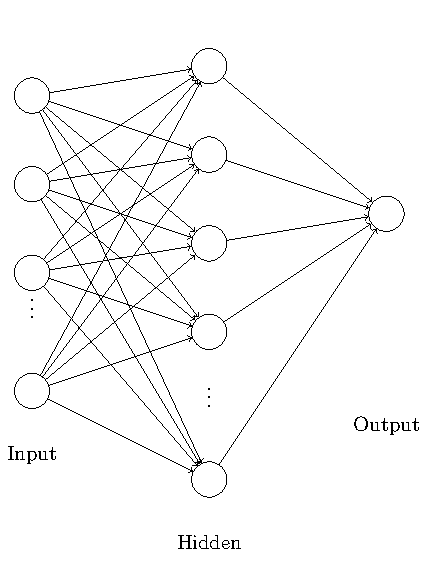
\includegraphics[width=\textwidth]{./project3/tikz/fnn.pdf}
        \caption{FNN}
        \label{subfig:fnn}
    \end{subfigure}
    \hspace{1cm}
    \begin{subfigure}{0.45\textwidth}
        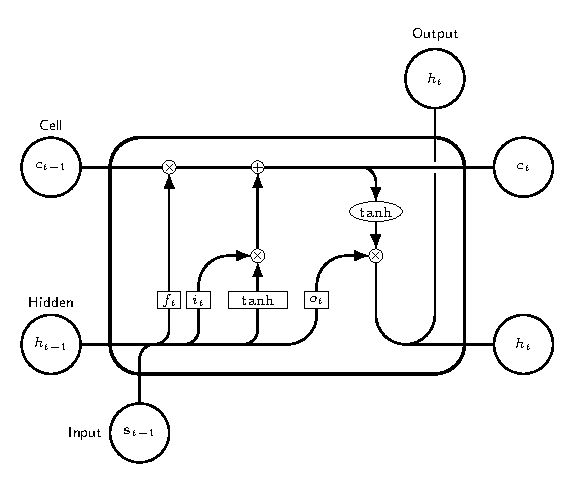
\includegraphics[width=\textwidth]{./project3/tikz/lstm.pdf}
        \caption{LSTM}
        \label{subfig:lstm}
    \end{subfigure}
    \caption{Neural Network Architectures}
    \label{fig:nn}
\end{figure}

Figure~\ref{subfig:fnn} shows a feedforward neural network (FNN) architecture with one hidden layer.
The input layer receives the input features, which are then passed through the hidden layer(s) to the output layer.
Each layer consists of multiple neurons, which apply a non-linear activation function to the weighted sum of the inputs.

\begin{equation}
    f(x; \theta) = f^{(k)}(f^{(k-1)} \cdots (f^{(2)}(f^{(1)}(x;\theta^{(1)});\theta^{(2)} )\cdots ;\theta^{(k-1)});\theta^{(k)}),
\end{equation}

where $\theta = (\theta^{(1)}, \theta^{(2)}, \ldots, \theta^{(k)})$ are the trainable parameters of the neural network, $f^{(i)}$ is the $i$-th layer of the neural network, $x$ is the input feature vector, $f^{(1)}(x;\theta^{(1)}) = x$, $f^{(k)}$ is the output layer, $k$ is the number of layers, and $f^{(i)}$ is the output of the $i$-th layer.
To move from a lower layer to a higher layer, i.e., from layer $i-1$ to layer $i$,

\begin{equation} \label{eq:neural}
    f^{(i)}(z;\theta^{(i)}) = a^{(i)}(\beta_0^{(i)} + \sum_{j=1}^{p_i} \beta_j^{(i)} z),
\end{equation}

where $a^{(i)}$ are the nonlinear activation functions, $\theta^{(i)} = (\beta_0^{(i)}, \dots, \beta_p^{(i)})$ are the trainable parameters of the $i$-th layer, and $p_i$ is the number of neurons in the previous layer.
Equation~\ref{eq:neural} represents a single neuron in a neural network, which applies a linear transformation to the input followed by a non-linear activation function. 
The linear transformation is similar to the linear regression model in Equation~\ref{eq:regression}, but the non-linear activation function allows the neural network to model complex, non-linear relationships in the data.
The FNN is tuned by adjusting the trainable parameters $\theta$ while fixing the activation functions $a^{(i)}$.
A typical choice for the activation function is the rectified linear unit (ReLU), which is defined as $a(z) = \max(0, z)$~\citep{nair2010rectified}.
The choice of activation function also plays a crucial role in the training of neural networks.
While sigmoid and hyperbolic tangent functions were popular in early neural networks, ReLU has become the default activation function for deep networks due to its ability to mitigate the vanishing gradient problem and promote sparse activations~\citep{lecun2015deep}.

The key advantage of feedforward neural networks (FNNs) lies in their ability to perform automatic feature engineering without direct human intervention. 
Unlike traditional machine learning models that require manual selection and transformation of input features, neural networks learn to extract and compose features through their hidden layers during the training. 
Each hidden layer in the network captures higher-level abstractions of the input data by transforming the outputs of the previous layer through nonlinear activation functions~\citep{lecun2015deep}.
Each layer builds upon the representations learned by the previous layer, enabling the network to capture multiple levels of abstraction. 
This characteristic is crucial for modeling complex datasets with intricate patterns and relationships~\citep{bengio2013representation}.

The last layer of the neural network, known as the output layer, typically performs a linear transformation of the features extracted by the preceding hidden layers. 
With $a^{k}(z) = z$, the last layer is equivalent to a linear regression with its inputs as transformed, high-level features learned by the hidden layers.
We can draw parallels between neural networks and traditional regression models. 
The main difference is that, in neural networks, the input features to the regression model are learned automatically rather than being manually specified.

The most well-known theorem in neural network theory is the universal approximation theorem~\citep{hornik1989multilayer}.
It states that given appropriate activation functions $a$, a feedforward neural network with a single hidden layer containing a finite number of neurons can approximate any continuous function on a compact subset of $\mathbb{R}^n$ to arbitrary accuracy. 
Despite this theoretical guarantee for single-layer neural networks, in practice, deep neural networks (DNN) with multiple hidden layers have been shown to be more effective at capturing complex patterns and relationships in data~\citep{lecun2015deep}.
Examples include AlexNet~\citep{krizhevsky2012imagenet}, VGG~\citep{simonyan2014very}, and ResNet~\citep{he2016deep}, which have achieved state-of-the-art performance on image classification tasks.
In this thesis, we focus on the application of deep neural networks, specifically long short-term memory (LSTM) networks, as metamodels for nested simulation procedures in risk management applications.

\subsection{Training and Evaluation of Neural Networks}

The training of neural networks involves adjusting the trainable parameters of the network to minimize the loss function, which quantifies the error between the predictions and labels.
The training process aims to find the optimal parameters that minimize this error.
The most common approach is to use gradient descent methods with backpropagation, which is an efficient method for computing the gradients of the loss function with respect to the trainable parameters.
Backpropagation computes the gradients by propagating the error derivatives backward through the network layers.
This process allows the network to adjust the parameters in the direction of minimizing the loss function.
The training process is typically performed over a number of epochs, where each epoch is one complete pass through the training dataset.

However, the training of neural networks is non-convex, and the optimization problem is challenging.
Stochastic gradient descent (SGD) is a popular optimization algorithm for training neural networks.
It updates the parameters using a single or a small batch of training examples at a time, which makes it much faster than the crude gradient descent.
However, SGD may oscillate and converge slowly, especially in non-convex problems~\citep{bengio2016}.
To address these issues, various adaptive learning rate methods have been proposed.
The most popular approach is Adam, which is a SGD algorithm that adjusts the learning rate during training to improve convergence speed and stability~\citep{kingma2014adam}.

Another common technique to improve the training of neural networks is regularization to prevent overfitting.
One effective regularization method is dropout, which randomly sets a fraction of neurons to zero during each training iteration~\citep{srivastava2014dropout}.
This prevents neurons from co-adapting too much, encourages redundancy, and leads to a more robust model that generalizes better to unseen data.
Early stopping is another regularization method that is relevant to our study.
It involves monitoring the model's performance on a validation set and stopping training when the performance no longer improves~\citep{prechelt2002early}.
This helps prevent over-fitting by stopping training before the model begins to fit to noise in the data.

Evaluation of the performance of a neural network is challenging due to the absence of analytical tools.
Existing machine learning literature addresses this challenge by splitting the data into three parts: training set, validation set, and test set.
The training set is used to train the model, the validation set is used to tune the model hyper-parameters, and the test set is used to evaluate how well the model generalizes to unseen data.
The test set is not used during training and is only used for evaluation.

Under-fitting occurs when the training error is high, which means that the neural network fails to capture the underlying patterns in the training data.
Over-fitting occurs when the neural network fits to noise in the training data and cannot generalize to unseen data.
In machine learning literature, over-fitting is often quantified as the gap between the training error and the test error~\citep{bishop2006pattern}.
During training, as the test dataset is not used, this quantity is estimated using the validation set.
If the validation error is high compared to the training error, the model is likely over-fitting to the training data.

\subsection{Long Short-Term Memory Networks}

Building upon the capabilities of FNNs, we recognize that while FNNs are successful at capturing complex, nonlinear relationships through automatic feature learning, they are inherently limited when it comes to modeling sequential data or time-dependent patterns. 
This independence assumption limits their effectiveness in modeling financial time series, where temporal dependencies play a critical role. 
The stylized facts of financial time series, such as volatility clustering, fat tails, and autocorrelation, are challenging to capture with traditional FNNs due to the absence of memory in the model~\citep{cont2001empirical}.

To overcome the limitations of FNNs in handling sequential input, recurrent neural networks (RNNs) were introduced.
In a RNN, the hidden state at each time step is a function of both the current input and the hidden state from the previous time period~\citep{elman1990finding}:

\begin{equation}
    h_t = f(x_t, h_{t-1}; \theta),
\end{equation}

where $h_t$ is the hidden state at time $t$, $x_t$ is the input at time $t$, $h_{t-1}$ is the hidden state at time $t-1$, and $f$ is the recurrent function parameterized by $\theta$.
This architecture enables RNNs to capture temporal dependencies by maintaining a dynamic internal state that reflects the memory of past inputs.
However, traditional RNNs suffer from the vanishing and explodeing gradient problem, which hinders their ability to capture long-term dependencies that often present in financial time series~\citep{bengio1994learning}.
During training, gradients propagated backward through time can either diminish exponentially (vanishing gradients) or grow uncontrollably (exploding gradients).
This limitation is particularly problematic in modeling long-term financial contracts and insurance guarantees, where patterns may span over extended periods.

To address these issues, a long short-term memory (LSTM) network was developed by \citet{hochreiter1997long}.
It is a specialized form of RNNs designed to capture long-term dependencies more effectively with the help of RNN memory cells and gating mechanisms.

\begin{align*}
    i_t &= a(W_i x_t + U_i h_{t-1} + b_i), \\
    f_t &= a(W_f x_t + U_f h_{t-1} + b_f), \\
    o_t &= a(W_o x_t + U_o h_{t-1} + b_o), \\
    g_t &= a(W_g x_t + U_g h_{t-1} + b_g), \\
    c_t &= f_t \odot c_{t-1} + i_t \odot g_t, \\
    h_t &= o_t \odot \tanh(c_t),
\end{align*}

where $i_t, f_t, o_t, g_t, c_t, h_t$ are the input gate, forget gate, output gate, cell input, cell state, and hidden state at time $t$, respectively.
$W_i$, $W_f$, $W_o$, $W_g$, $U_i$, $U_f$, $U_o$, $U_g$ are the weight matrices, and $b_i$, $b_f$, $b_o$, $b_g$ are the bias vectors.
$a$ is the activation function, typically the sigmoid function, and $\odot$ denotes element-wise multiplication.

\begin{equation*}
    a(z) = \frac{1}{1 + e^{-z}}.
\end{equation*}

Figure~\ref{subfig:lstm} shows the architecture of an LSTM network.
The gating mechanisms in LSTM networks effectively mitigate the vanishing and exploding gradient problem by regulating the flow of information through the network.
The input gate $i_t$ controls the flow of information into the cell state $c_t$, the forget gate $f_t$ regulates the retention of information in the cell state, and the output gate $o_t$ determines the information passed to the hidden state $h_t$.
The cell input $g_t$ is used to update the cell state based on the input $x_t$ and the previous hidden state $h_{t-1}$.
The cell state $c_t$ acts as a memory unit that stores information over time, while the hidden state $h_t$ captures the relevant information for the current time step.
By incorporating memory cells and gating mechanisms, LSTMs can effectively model long-term dependencies in sequential data in finance and actuarial applications.

The advancements in neural network optimization techniques, architectures, and training methodologies have significantly enhanced their usefulness in risk management applications.
By effectively modeling complex, non-linear relationships and temporal dependencies, neural networks serve as powerful tools for addressing the computational challenges in estimating risk measures and developing effective risk mitigation strategies.
This thesis aims to explore the application and noise tolerance of LSTM networks in metamodeling for nested simulation procedures in risk management.
We investigate the performance of LSTM networks in approximating the inner simulation model in a two-stage nested simulation procedure for index-linked insurance contracts.
By leveraging the memory and sequential modeling capabilities of LSTMs, we aim to improve the accuracy and efficiency of nested simulation procedures for risk management applications.


%======================================================================
\chapter{Nested Simulation Procedures in Financial Engineering: A Selected Review}
%======================================================================


\section{Introduction}

Nested simulation procedures are commonly used in financial engineering to estimate risk measures for portfolios of complex financial derivatives. 
The term \textit{nested} is referred to a nested estimation problem, in which the estimation of the risk measure requires two levels of Monte Carlo (MC) simulations.
In a typical nested simulation procedure, an outer level simulation model generates underlying risk factors, which is referred to as the \textit{outer scenarios}.
For each outer scenario, an inner level simulation model generates scenario-wise samples of the portfolio losses, which is referred to as the \textit{inner replications}.

The nested simulation procedure is computationally expensive due to its nested structure. 
Given a fixed computational budget, the nested simulation procedure has to make a trade-off between the number of outer scenarios and the number of inner replications.
~\cite{gordy2010nested} are the first to analyze and propose the optimal budget allocation of a standard nested simulation procedure. 
The term \textit{standard} refers to using a standard Monte Carlo estimator, the sample mean of the inner replication to estimate a scenario-wise portfolio loss for an outer scenario.
~\cite{gordy2010nested} investigate the optimal budget allocation for a standard nested simulation procedure with respect to the mean squared error (MSE) of the estimated risk measure.

The standard nested simulation procedure is computationally expensive with a somewhat wasteful use of the simulation budget, as only the inner replications from the same outer scenario are used in estimating the scenario-wise portfolio loss for that outer scenario. 
Subsequent research efforts have been made to improve the efficiency of nested simulation procedures by using the inner replications from other outer scenarios. 
This is referred to as pooling. 
Different methods pool in different ways, either by a trained proxy model or by pre-defined likelihood ratio weights.
~\cite{broadie2015risk} propose a regression-based nested simulation procedure, which uses a trained regression proxy model to estimate the scenario-wise portfolio loss for an outer scenario by pooling the inner replications from all outer scenarios.
For risk measures in certain forms,~\cite{broadie2015risk} show that it is optimal to allocate all simulation budget to the outer level simulation, and the inner replication should be kept to a minimum of $1$.
Similarly,~\cite{hong2017kernel},~\cite{feng2020optimal}, and~\cite{zhang2022sample} use a kernel smoothing model, a likelihood ratio model, and a kernel ridge regression model as proxies to pool the inner replications from all outer scenarios.
In simulation studies, this approach of using a model of a simulation model is known as metamodeling, and the models of a simulation model are also referred to as metamodels~\citep{barton1998simulation}.
Another line of research is the multi-level Monte Carlo (MLMC) method analyzed in~\cite{giles2019multilevel}, which is a variance reduction technique that uses a hierarchy of approximations to the quantity of interest.

This paper presents a survey study of some popular nested simulation procedures. 
Many procedures are proposed in the literature, but they are not directly comparable due to different error metrics, different assumptions, and different numerical examples.
Within a common analytical framework, we first summarize and compare their asymptotic rate of convergence.
Their asymptotic convergence results are closely examined for their assumptions that guarantee the convergence.
Furthermore, our study finds that different studies propose different examples in their numerical experiments, which introduces unfair advantages for certain simulation procedures over others. 
A fair comparison among popular methods is therefore urgently needed in the literature. 
Our numerical experiment is the first of its kind to subject back all the aforementioned simulation procedures to a complete and unbiased comparison. 
Extensive numerical experiments are conducted to show, in practical examples, how well the finite-sample performance of a method matches its theoretical convergence behavior. 
With our numerical examples, we compare the nested simulation procedures for different payoff complexity, problem dimensions, and risk measures. 

The rest of the paper is organized as follows.
Section~\ref{sec1:problem-formulation} introduces the nested simulation procedure and the standard Monte Carlo estimator.
Section~\ref{sec1:asymptotic-convergence} provides new theoretical results on the convergence of existing nested simulation procedures.
Section~\ref{sec1:convergence-orders} summarizes the asymptotic convergence orders and the critical assumptions of nested simulation procedures in the literature.
Section~\ref{sec1:numerical-experiments} presents the numerical experiments and the comparisons of different nested simulation procedures with respect to different risk measures, problem dimensions, and payoff complexities.
Section~\ref{sec1:computational-complexity} discusses the computational complexity of different nested simulation procedures.
Section~\ref{sec1:conclusion} concludes the paper.

\section{Problem Formulation} \label{sec1:problem-formulation}

In a nested estimation problem, we are interested in the quantity 

$$\rho(g(X)), $$

where $X \in \Omega$. 
$g(X)$ can't be directly evaluated, but it is the output of 

$$ g(X) = \mathbb{E}\left[ Y|X=x \right]\vert_{x=X} $$

Some common risk measures are in the nested expectation form, in which 
$$\rho(g(X)) = \mathbb{E}\left[ h(g(X)) \right]$$

where $h(\cdot)$ is a known function. 
Forms of $h$ include the following:
\begin{itemize}
    \item 	Smooth functions, e.g., a quadratic tracking error with benchmark $b$: $h(t) = (t - b)^2$
    \item 	Lipschitz continuous functions, e.g., a mean excess loss over threshold $u$: $h(t) = \max\{t - u, 0\}$. Here, $h$ is a hockey-stick function.
    \item 	Indicator functions, e.g., probability of a large loss over a threshold $u$: $h(t) = \mathbb{I}_{\{t \geqslant u\}}$
\end{itemize}

Other risk measures of interest that are not in the nested expectation form are the value at risk (VaR) and the conditional value at risk (CVaR). 
The $\alpha$-VaR of $g(X)$ is defined as
$$
    \mbox{VaR}_\alpha(g(X)) = q_\alpha = \inf \left\{ q: \Pr(g(X)\leq q) \geq \alpha \right\}.
$$
The $\alpha$-CVaR of $g(X)$ is defined as
$$
    \mbox{VaR}_\alpha(g(X)) =\frac{1}{1-\alpha} \int_{\alpha}^{1} q_v dv. 
$$

\subsection{The Standard Nested Simulation Procedure}

The standard nested simulation procedure first simulates $M$ independent and identically distributed (iid) outer scenarios $X_1, \dots, X_M$ from $F_X$, the distribution of $X$.
For each $X_i$, again simulate $Y_{ij}$, $j = 1, \dots, N$ from $F_{Y|X_i}$, the conditional distribution of $Y$ given $X_i$. Given scenario $i$, the $Y_{ij}$ are conditionally iid. Let $\Gamma = M \cdot N$ denote the total simulation budget, $f_X(x)$ denote the density of $X$, and $\mathbf{X} = (X_1, \dots, X_M)$ denote the vector of outer scenarios.

The standard nested simulation procedure estimates $g(X_i)$ with a standard Monte Carlo estimator 

$$\hat{g}_N(X_i) = \frac{1}{N} \sum_{j=1}^N Y_{ij}; ~~~ Y_{ij} \sim F_{Y|X_i} $$

Let $(\hat{g}_N(\mathbf{X}))_{[1]}, \dots, (\hat{g}_N(\mathbf{X}))_{[M]}$ be the order statistics of $\hat{g}_N(X_1), \dots \hat{g}_N(X_M)$. 
The standard nested simulation estimators for different forms of $\rho$ are as follows:

\begin{enumerate}
    \item   Nested expectation form:
            $$\hat{\rho}_{M, N} = \frac{1}{M} \sum_{i=1}^M h(\hat{g}_N(X_i)) = \frac{1}{M} \sum_{i=1}^M h(\bar{Y}_{N, i}); ~~~ X_i \sim F_X$$
    \item   Value at risk (VaR):
            $$\hat{\rho}_{M, N} = (\hat{g}_N(\mathbf{X}))_{\lceil \alpha M \rceil}$$
    \item   Conditional value at risk (CVaR):
            $$\hat{\rho}_{M, N} = (\hat{g}_N(\mathbf{X}))_{\lceil \alpha M \rceil} + \frac{1}{(1-\alpha) M} \sum_{i=1}^M \max \{\hat{g}_N(X_i) - (\hat{g}_N(\mathbf{X}))_{\lceil \alpha M \rceil}, 0 \}$$
\end{enumerate}

~\cite{gordy2010nested} analyze the optimal budget allocation of the standard nested simulation procedure with respect to the MSE of the estimator $\hat{\rho}_{M, N}$.


\subsection{Multi-level Monte Carlo}

The multi-level Monte Carlo (MLMC) method is a variance reduction technique that uses a hierarchy of approximations to the quantity of interest, and it uses the difference between the approximations to reduce the variance of the estimator.
The MLMC method is particularly useful when the quantity of interest is expensive to evaluate, and the standard Monte Carlo estimator has a high variance.
The MLMC method estimates $\rho$ with a multi-level Monte Carlo estimator:

\begin{equation*}
    \hat{\rho}^{\text{MLMC}}_\Gamma = \sum_{\ell=0}^{L} \left( \frac{1}{M_{\ell}} \sum_{i=1}^{M_{\ell}} h(\hat{g}_{N_{\ell}}(X_{i, \ell})) - \frac{1}{M_{\ell-1}} \sum_{i=1}^{M_{\ell-1}} h(\hat{g}_{N_{\ell-1}}(X_{i, \ell-1})) \right), ~~~ X_{i, \ell} \sim F_X,
\end{equation*}

where $\hat{g}_N(\cdot) = 0$, $L$ is the number of levels, $M_{\ell}$ is the number of outer scenarios at level $\ell$, and $N_{\ell}$ is the number of inner replications at level $\ell$.
Applying the analysis of~\cite{giles2015multilevel} in a nested simulation context,~\cite{giles2019multilevel} show that the MLMC method can achieve a similar level of accuracy as the standard nested simulation procedure with a lower total computational budget.
The simulation budget $\Gamma$ is the sum of the computational budget at each level, that is, $\Gamma = \sum_{\ell=0}^{L} M_{\ell} \cdot N_{\ell}$.

\subsection{Supervised Learning Models}

In supervised learning, $g(\cdot)$ can be approximated by $\hat{g}^{\text{SL}}_{M, N}(\cdot)$, which is based on a chosen function family $\mathcal{G}$ and observations from the standard nested simulation procedure.
Consider the observation pairs $(X_i, \hat{g}_N(X_i))$ for $i \in \{1, \dots, M\}$ as training data, we can use supervised learning to approximate $g(\cdot)$ by $\hat{g}^{\text{SL}}_{M, N}(\cdot)$ and to pool the inner replications from all outer scenarios.
Using the $M$ \textit{training} samples, a nested Monte Carlo estimator of $\rho$ is given by

\begin{enumerate}
    \item   Nested expectation form:
            $$\hat{\rho}^{\text{SL}, \text{Train}}_{M, N} = \frac{1}{M} \sum_{i=1}^M h(\hat{g}^{\text{SL}}_{M, N}(X_i)); ~~~ X_i \sim F_X$$
    \item   VaR:
            $$\hat{\rho}^{\text{SL}, \text{Train}}_{M, N} = (\hat{g}^{\text{SL}}_{M, N}(\mathbf{X}))_{\lceil \alpha M \rceil}$$
    \item   CVaR:
            $$\hat{\rho}^{\text{SL}, \text{Train}}_{M, N} = (\hat{g}^{\text{SL}}_{M, N}(\mathbf{X}))_{\lceil \alpha M \rceil} + \frac{1}{(1-\alpha) M} \sum_{i=1}^M \max \{\hat{g}^{\text{SL}}_{M, N}(X_i) - (\hat{g}^{\text{SL}}_{M, N}(\mathbf{X}))_{\lceil \alpha M \rceil}, 0 \}$$
\end{enumerate}
where $(\hat{g}_{M, N}(\mathbf{X}))_{\lceil \alpha M \rceil}$ is the $\lceil \alpha M \rceil$-th order statistic of $\hat{g}^{\text{SL}}_{M, N}(X_1), \dots, \hat{g}_{M, N}(X_M)$.
Similarly, with $M'$ \textit{test} samples of $X$, namely $\tilde{\mathbf{X}} = \tilde{X}_1, \dots, \tilde{X}_{M'}$, an estimator is given by

\begin{enumerate}
    \item   Nested expectation form:
            $$\hat{\rho}^{\text{SL}, \text{Test}}_{M, N, M'} = \frac{1}{M'} \sum_{i=1}^{M'} h(\hat{g}^{\text{SL}}_{M, N}(\tilde{X}_i)); ~~~ \tilde{X}_i \sim F_X.$$
    \item   VaR:
            $$\hat{\rho}^{\text{SL}, \text{Test}}_{M, N, M'} = (\hat{g}^{\text{SL}}_{M, N}(\tilde{\mathbf{X}}))_{\lceil \alpha M' \rceil}.$$
    \item   CVaR:
            \begin{align*}
                \hat{\rho}^{\text{SL}, \text{Test}}_{M, N, M'} & = (\hat{g}^{\text{SL}}_{M, N}(\tilde{\mathbf{X}}))_{\lceil \alpha M' \rceil}  \\
                & + \frac{1}{(1-\alpha) M'} \sum_{i=1}^{M'} \max \{\hat{g}^{\text{SL}}_{M, N}(\tilde{X}_i) - (\hat{g}^{\text{SL}}_{M, N}(\tilde{\mathbf{X}}))_{\lceil \alpha M' \rceil}, 0 \}, 
            \end{align*}
\end{enumerate}
where $(\hat{g}_{M, N}(\tilde{\mathbf{X}}))_{\lceil \alpha M' \rceil}$ is the $\lceil \alpha M' \rceil$-th order statistic of $\hat{g}^{\text{SL}}_{M, N}(\tilde{X}_1), \dots, \hat{g}_{M, N}(\tilde{X}_{M'})$. 
Note that $\hat{g}^{\text{SL}}_{M, N}(\cdot)$ is derived from the training samples $(X_1, \hat{g}_N(X_1)), \dots, (X_M, \hat{g}_N(X_M))$. 

We are interested in minimizing the MSE of the supervised learning-based nested simulation estimator with supervised learning $\hat{\rho}^{\text{SL}, \text{Train}}_{M, N}$ and $\hat{\rho}^{\text{SL}, \text{Test}}_{M, N, M'}$ subject to the total simulation budget $\Gamma$.

\begin{align}
    & \min_{M, N}  & \text{MSE}(\hat{\rho}^{\text{SL}}_{M, N}) = \mathbb{E} \left[ \left( \hat{\rho}^{\text{SL}}_{M, N} - \rho \right)^2 \right] \nonumber \\
    & \text{subject to} & M \cdot N = \Gamma 
\end{align}

Existing literature on nested simulation procedures has proposed different methods to approximate the true function $g(\cdot)$ with supervised learning algorithms. 
Methods that include theoretical convergence results are regression~\citep{broadie2015risk}, kernel smoothing~\citep{hong2017kernel}, and kernel ridge regression~\citep{wang2022smooth}.
Their estimators of $g(\cdot)$ are given by $\hat{g}^{\text{REG}}_{M, N}(\cdot)$, $\hat{g}^{\text{KS}}_{M, N}(\cdot)$, and $\hat{g}^{\text{KRR}}_{M, N}(\cdot)$, respectively.

\begin{itemize}
    \item   Regression:
            $$\hat{g}^{\text{REG}}_{M, N}(X) = \Phi(X) \hat{\beta},$$
            where $\Phi$ is a chosen basis, and $\hat{\beta}$ is estimated from the training samples.
    \item   Kernel smoothing:
            $$\hat{g}^{\text{KS}}_{M, N}(X) = \frac{\sum_{i=1}^M \bar{Y}_{N, i} K_w(X - X_i)}{\sum_{i=1}^M K_w(X - X_i)}, $$
            where $K_w$ is the kernel function with bandwidth $w$.
    \item   Kernel ridge regression:
            $$\hat{g}^{\text{KRR}}_{M, N}(X) = \argmin_{g \in \mathcal{N}_{\Psi}(\Omega)} \left( \frac{1}{M} \sum_{i=1}^M (\hat{g}_N(X_i) - g(X_i))^2 + \lambda \|g\|_{\mathcal{N}_{\Psi}(\Omega)}^2\right),$$
            where $\mathcal{N}_{\Psi}(\Omega)$ is the reproducing kernel Hilbert space (RKHS) with kernel $\Psi$ defined domain $\Omega$, and $\lambda$ is the regularization parameter as in ridge regression. 
            More specifically, $\Phi$ is a Mat\'ern kernel with smoothness parameter $\nu$ and length scale parameter $\ell$.
\end{itemize}

\subsection{Likelihood Ratio Method}

Instead of using a supervised learning model as proxy,~\cite{zhang2022sample} uses the likelihood ratio weights to pool the inner replications from all outer scenarios.
Here, we restrict our attention to problems in the nested expectation form whose outer scenarios characterize the stochasticity of the inner simulation model. 
Specifically,
$$ Y = Y(H, X), $$
where $H$ is a random variable whose distribution is specified by the outer scenarios $X$. 
We denote the conditional distribution of $H|X$ by $f_{H|X}$. 
For a specific scenario $X_i$, we write $f_{H|X}(\cdot |X_i)$. 
To reconcile with previously established notations, we note that inner simulation outputs $Y_{ij}$ can be written as
$$ Y_{ij} = Y(H_{ij}, X_i), $$
where $H_{ij} \sim f_{H|X}(\cdot |X_i)$.
Suppose that one can generate random variable H from some sampling
distribution $f_H$. Then, the likelihood ratio estimator of $\rho$ is given by
$$\hat{\rho}^{\text{LR}}_{M,N} = \frac{1}{M} \sum_{i=1}^M h(\hat{g}^{\text{LR}}_N(X_i)), $$ where the inner replications are pooled by the likelihood ratio weights with
$$\hat{g}^{\text{LR}}_N(X_i) = \frac{1}{N} \sum_{j=1}^N Y(H_j, X_i) \frac{f_{H|X}(H_{j}|X_i)}{f_H(H_{ij})}, \;\;\; H_j \sim f_H, \;\;\; i=1, \dots, M.$$

With a total simulation budget $\Gamma$, we are interested in the order of convergence of estimators for all nested simulation procedures, which is measured by their MSE about the risk measure $\rho$.

\begin{align}
    & \min ~~~ \mathbb{E} \left[ \left( \hat{\rho}_{M, N} - \rho \right)^2 \right] \nonumber \\
    & \text{subject to} ~~~ M \cdot N = \Gamma, 
\end{align}

where $\Gamma$ is the total simulation budget for all nested simulation procedures considered in this study.
A special case is the MLMC method, where the total simulation budget $\Gamma$ is the sum of the computational budget at all levels.

\section{Asymptotic Analysis} \label{sec1:asymptotic-convergence}
In this section, we summarize the existing asymptotic convergence results of the nested simulation procedures in the literature, and we compare their critical assumptions that guarantee the convergence.

\begin{table}[ht]
    \centering
    \footnotesize
    \begin{tabular}{|l|c|c|c|c|c|}
    \hline
    \textbf{Estimator for} $g(X)$ & \textbf{Smooth} $h$ & \textbf{Lipschitz}(\textbf{hockey-stick} $h$) & \textbf{Indicator} $h$ & \textbf{VaR} & \textbf{CVaR} \\
    \hline
    Standard Monte Carlo & $\star$ & $\star$($\checkmark$) & $\checkmark$ & $\checkmark$ & $\times$ \\
    \hline
    Multi-level Monte Carlo & $\times$ & $\times$($\times$) & $\checkmark$ & $\times$ & $\times$ \\
    \hline
    Regression & $\checkmark$ & $\checkmark$($\checkmark$) & $\times$ & $\times$ & $\times$ \\
    \hline
    Kernel smoothing & $\checkmark$ & $\times$($\checkmark$) & $\checkmark$ & $\times$ & $\times$ \\
    \hline
    Kernel ridge regression & $\Diamond$ & $\times$($\Diamond$) & $\Diamond$ & $\Diamond$ & $\Diamond$ \\
    \hline
    Likelihood ratio & $\checkmark$ & $\times$($\checkmark$) & $\checkmark$ & $\times$ & $\times$ \\
    \hline
    \end{tabular}
    \caption{Existing asymptotic convergence results of nested simulation procedures for MSE}
    \label{tab1:asymConv-mse}
\end{table}


Table~\ref{tab1:asymConv-mse} summarizes the existing asymptotic convergence results of nested simulation procedures for MSE in the literature.
A $\checkmark$ indicates there exists an asymptotic convergence result for the corresponding estimator,
a $\times$ indicates there does not exist an asymptotic convergence result, 
a $\star$ indicates an asymptotic result is not available in the literature but is provided in this study, and
a $\Diamond$ indicates the asymptotic convergence result exists in the literature but in a weaker form.
~\cite{gordy2010nested} provide the asymptotic convergence results for the standard nested simulation procedure with hockey-stick $h$, indicator $h$ and VaR.
Their CVaR analysis is incomplete as the VaR is assumed to be known but not estimated in the convergence proof.
When the VaR is known, the CVaR analysis reduces to the nested expectation form with $h$ being a hockey-stick function.
~\cite{giles2019multilevel} provide the asymptotic convergence results for the MLMC method with an indicator $h$.
~\cite{broadie2015risk} provide the asymptotic convergence results for the regression-based nested simulation procedure with smooth $h$ and Lipschitz continuous $h$.
The Lipschitz continuous family includes the hockey-stick function as a special case, thus the convergence result for the hockey-stick function is implied.
~\cite{hong2017kernel} and~\cite{zhang2022sample} provide the asymptotic convergence results with the nested expectation form for the kernel smoothing-based procedure and likelihood ratio-based nested simulation procedure, respectively.
The convergence results for a Lipschitz continuous $h$ cannot be directly inferred from the analysis for a hockey-stick function.

While most of the literature focuses on the MSE of the estimator of $\rho$,~\cite{wang2022smooth} analyze the asymptotic convergence of the estimator of $\rho$ in terms of the absolute error.
Let $\hat{\rho}$ be the estimator of $\rho$. Its absolute error about $\rho$ is defined as

$$
\mbox{Absolute Error}\left(\hat{\rho}\right) = \left| \hat{\rho} - \rho \right|.
$$

In~\cite{wang2022smooth}, the authors of the KRR-based nested simulation procedures claim to have bridged the gap between the cubic and square root convergence rates of nested simulation procedures. However, they analyze convergence in probabilistic order, and it is only applicable in terms of the absolute error. 
Instead of showing the convergence of the KRR-based estimator in terms of MSE as in~\cite{gordy2010nested}, we show the connections between the convergence in MSE and the convergence in probabilistic order for absolute error.
Our findings in Section~\ref{sec1:connection-mse-absolute-error} show that the analysis of ~\cite{wang2022smooth} indeed bridges the gap, but only in terms of the absolute error.

\subsection{Connections between Convergence in MSE and Absolute Error} \label{sec1:connection-mse-absolute-error}

This section establishes the connections between the convergence in MSE and the convergence in probabilistic order for absolute error in the context of nested simulation procedures.
In order to show the connections between the convergence in MSE and the convergence in probabilistic order for absolute error, we first need to state the definition for a sequence of random variables to converge in those two forms.

\begin{definition}
    Let $\hat{\rho}_{\Gamma}$ be an estimator of $\rho$ with a simulation budget of $\Gamma$. 
    We write $\mathbb{E} \left[ \left(\hat{\rho}_{\Gamma} - \rho\right)^2 \right] = \mathcal{O} \left( \Gamma^{-k} \right)$, that is, $\hat{\rho}_{\Gamma}$ converges in MSE to $\rho$ in order $k$ if 
    $$
        \exists C \limsup_{M} \frac{\mathbb{E} \left[\left(\hat{\rho}_{\Gamma} - \rho\right)^2 \right]}{\Gamma^{-k}} \leq C
    $$
\end{definition}

\begin{definition}
    Let $\hat{\rho}_{\Gamma}$ be an estimator of $\rho$ with a simulation budget of $\Gamma$. 
    We write $|\hat{\rho}_{\Gamma} - \rho| = \mathcal{O}_{\mathbb{P}}(\Gamma^{-k})$, that is $\hat{\rho}_{\Gamma}$ converges in probabilistic order $k$ to $\rho$ if for large enough $\Gamma$,
    $$
        \forall \epsilon > 0 \exists C \mathbb{P} \left( \left| \hat{\rho}_{\Gamma} - \rho \right| \geq C \Gamma^{-k} \right) \leq \epsilon 
    $$
\end{definition}

We start by showing the convergence in probabilistic order from the convergence in MSE.
Let $\hat{\rho}_{\Gamma}$ be an estimator of $\rho$ with a simulation budget of $\Gamma$, and assume that $\mathbb{E} \left[ \left(\hat{\rho}_{\Gamma} - \rho\right)^2 \right] = \mathcal{O} \left( \Gamma^{-k} \right)$.
Then, from the definition of convergence in MSE, there exists a constant $C$ such that 
$$
    \limsup_{M} \frac{\mathbb{E} \left[ \left(\hat{\rho}_{\Gamma} - \rho\right)^2 \right]}{\Gamma^{-k}} \leq C.
$$
Hence, there exists some $\Gamma$ such that for all $\gamma \geq \Gamma$,
$$
\mathbb{E} \left[ \left(\hat{\rho}_{\gamma} - \rho\right)^2 \right] \leq C\gamma^{-k}.
$$
The convergence in probabilistic order can be shown by separating the expectation into two parts: tail and non-tail.
$$
\mathbb{E} \left[ \left(\hat{\rho}_{\gamma} - \rho\right)^2 \cdot \mathbb{I}_{\{|\hat{\rho}_{\gamma} - \rho| \leq d\gamma^s\}} \right] + \mathbb{E} \left[ \left(\hat{\rho}_{\gamma} - \rho\right)^2 \cdot \mathbb{I}_{\{|\hat{\rho}_{\gamma} - \rho| > d\gamma^s\}} \right] \leq C\gamma^{-k}.
$$
The first term is always positive, and the second term can be bounded from below by the indicator function.
\begin{align*}
\mathbb{E} \left[ \left(\hat{\rho}_{\gamma} - \rho\right)^2 \cdot \mathbb{I}_{\{|\hat{\rho}_{\gamma} - \rho| > d\gamma^s\}} \right] 
& \geq \mathbb{E} \left[ d^2 \gamma^{2s} \cdot \mathbb{I}\{|\hat{\rho}_{\gamma} - \rho| > d\gamma^s\} \right] \\
& = d^2 \gamma^{2s} \cdot \mathbb{E} \left[ \mathbb{I}\{|\hat{\rho}_{\gamma} - \rho| > d\gamma^s \} \right] \\
& = d^2 \gamma^{2s} \cdot \mathbb{P} \left(|\hat{\rho}_{\gamma} - \rho| > d\gamma^s \right)
\end{align*}

Combining bounds on the two terms, we have

$$
    d^2 \gamma^{2s} \mathbb{P} \left(|\hat{\rho}_{\gamma} - \rho| > d\gamma^s \right) \leq C \gamma^{-k}.
$$

Let $s = -\frac{k}{2}$. Arranging the terms, we have

$$
    \mathbb{P} \left( |\hat{\rho}_{\gamma} - \rho| > d\gamma^{-\frac{k}{2}} \right) \leq \frac{C}{d^2}
$$

Hence, for all $\epsilon >0$, there exist $C^* = \sqrt{\frac{C}{\epsilon}}$ such that for all $\gamma \geq \Gamma$,

$$
    \mathbb{P} \left( |\hat{\rho}_{\gamma} - \rho| > C^*\gamma^{-\frac{k}{2}} \right) \leq \epsilon
$$

In essence, the above is the definition of convergence in probabilistic order, that is,

$$
    \left| \hat{\rho}_{\gamma} - \rho \right| = \mathcal{O}_\mathbb{P} \left( \Gamma^{-\frac{k}{2}} \right)
$$

\begin{theorem} \label{thm1:convergence-mse-prob}
    Let $\hat{\rho}_{\Gamma}$ be an estimator of $\rho$ with a simulation budget of $\Gamma$. 
    If $\hat{\rho}_{\Gamma}$ converges in MSE to $\rho$ in order $k$, then $\hat{\rho}_{\Gamma}$ converges in probabilistic order to $\rho$ in order $\frac{k}{2}$.
\end{theorem}

To the best of our knowledge, Theorem~\ref{thm1:convergence-mse-prob} has not been explicitly stated in the literature.
It is the first result that shows the connections between the convergence in MSE and the convergence in probabilistic order for absolute error in the context of nested simulation.
Theorem~\ref{thm1:convergence-mse-prob} is a general result that can be applied to any nested simulation procedure that converges in MSE to $\rho$ in order $k$.
If the estimator converges in MSE to $\rho$ in order $k$, then it converges in probabilistic order to $\rho$ in order $\frac{k}{2}$.

While the convergence in MSE implies the convergence in probabilistic order, the converse is not necessarily true.
Similarly, the above argument is applied in reverse.
Let $\hat{\rho}_{\Gamma}$ be an estimator of $\rho$ with a simulation budget of $\Gamma$, and assume that $|\hat{\rho}_{\Gamma} - \rho| = \mathcal{O}_{\mathbb{P}}(\Gamma^{-k})$.
The MSE of $\hat{\rho}_{\Gamma}$ can be separated into the same two parts.

$$
    \mathbb{E}\left[ \left(\hat{\rho}_{\Gamma} - \rho\right)^2 \right] = \mathbb{E} \left[ \left(\hat{\rho}_{\Gamma} - \rho\right)^2 \cdot \mathbb{I}_{\{|\hat{\rho}_{\Gamma} - \rho| \leq d\Gamma^{-2k}\}} \right] + \mathbb{E} \left[ \left(\hat{\rho}_{\Gamma} - \rho\right)^2 \cdot \mathbb{I}_{\{|\hat{\rho}_{\Gamma} - \rho| > d\Gamma^{-2k}\}} \right], 
$$
where the first term can be bounded from above.

\begin{align*}
    \mathbb{E} \left[ \left(\hat{\rho}_{\Gamma} - \rho\right)^2 \cdot \mathbb{I}_{\{|\hat{\rho}_{\Gamma} - \rho| > d\Gamma^s\}} \right] 
    & \leq d^2 \Gamma^{-2k} \cdot \mathbb{E} \left[ \mathbb{I}\{|\hat{\rho}_{\Gamma} - \rho| > d\Gamma^s \} \right] \\
    & = d^2 \Gamma^{-2k} \cdot \mathbb{P} \left(|\hat{\rho}_{\Gamma} - \rho| > d\Gamma^s \right) \leq d^2 \Gamma^{-2k} 
\end{align*}
However, the second term is not always bounded. 
If the random variable $\hat{\rho}_{\Gamma}$ admits a density function $f$, then the second term can be further decomposed.

\begin{align*}
    \mathbb{E} \left[ \left(\hat{\rho}_{\Gamma} - \rho\right)^2 \cdot \mathbb{I}_{\{|\hat{\rho}_{\Gamma} - \rho| > d\Gamma^{-2k}\}} \right] 
    & = \int_{-\infty}^{-d\Gamma^{-2k}} (x - \rho)^2 f(x) dx + \int_{d\Gamma^{-2k}}^{\infty} (x - \rho)^2 f(x) dx 
\end{align*}
Hence, $\hat{\rho}_{\Gamma}$ converges in MSE to $\rho$ in order $2k$ if and only if both integrals converge in order higher than $2k$. 
The above argument shows that the convergence in probabilistic order does not necessarily imply the convergence in MSE.
The convergence in probabilistic order is a weaker form of convergence than the convergence in MSE.

\subsection{Asymptotic Analysis for the Standard Nested Simulation Procedure}
In~\cite{gordy2010nested}, the authors analyze the asymptotic convergence of the standard nested simulation procedure in terms of MSE. 
The analysis is complete for the nested expectation form where $h$ is either an indicator function or a hockey-stick function and VaR. 
For the nested expectation form where $h$ is a smooth function or a Lipschitz continuous function, the analysis is incomplete.
In this section, we fill in the holes in the analysis of~\cite{gordy2010nested}.

\begin{assumption} \label{as1:sns}
    $h(g(X))$ has finite second moment, i.e., $\mathbb{E} \left[ \left( h(g(X)) \right)^2 \right] < \infty$.
\end{assumption}

\begin{assumption} \label{as1:sns-noise}
    $\hat{g}_N(X) = g(X) + \bar{Z}_N(X)$, where the simulation noise $\bar{Z}_N(X)$ has zero mean and variance $\nu(X) / N$, where the conditional variance $\nu(X)$ is bounded, i.e., there exists $C_{\nu, 1} > 0$ such that $\nu(x) \leq C_{\nu, 1}$ for all $x \in \mathbb{R}$. 
\end{assumption}

Let $\rho_M = \frac{1}{M} \sum_{i=1}^M h(g(X_i))$ be the nested Monte Carlo estimator with the true function $g$.
The MSE of the standard procedure can be decomposed into two terms.

\begin{align} \label{eq1:mse-sns}
    & \mathbb{E} \left[ \left( \hat{\rho}_{M, N} - \rho \right)^2 \right] \nonumber \\
    & \leq 2 \mathbb{E} \left[ \left( \hat{\rho}_{M, N} - \rho_M \right)^2 \right] 
            + 2  \mathbb{E} \left[ \left(\rho_M - \rho \right)^2 \right]  \nonumber \\
    & = 2 \mathbb{E} \left[  \left( \frac{1}{M} \sum_{i=1}^M h\left( \hat{g}_{N}(X_i) \right) -  \frac{1}{M} \sum_{i=1}^M h\left(g(X_i) \right)  \right)^2\right] \nonumber \\
    & ~~~~ + 2  \mathbb{E} \left[ \left(\frac{1}{M} \sum_{i=1}^M h\left(g(X_i) \right) - \mathbb{E}\left[ h(g(X))\right] \right)^2 \right]  \nonumber \\
    & = 2 \mathbb{E} \left[  \left( \frac{1}{M} \sum_{i=1}^M h\left( \hat{g}_{N}(X_i) \right) -  h\left(g(X_i) \right)  \right)^2\right] + \frac{2}{M} \text{Var}(h(g(X))) \nonumber \\
    & = 2 \mathbb{E} \left[  \left( \frac{1}{M} \sum_{i=1}^M h\left( \hat{g}_{N}(X_i) \right) -  h\left(g(X_i) \right)  \right)^2\right] + \mathcal{O}(M^{-1}),
\end{align}
where the last equality follows from Assumption~\ref{as1:sns}.
The analysis of the first term is different for smooth and Lipschitz continuous $h$. 
We will analyze them separately.

\subsubsection*{A Smooth Function $h$}
\begin{assumption} \label{as1:sns-smooth}
    The function $h$ has bounded first and second order derivative, i.e., there exists $C_1 > 0$ such that $|h'(x)| \leq C_1$ for all $x \in \mathbb{R}$, and there exists $C_2 > 0$ such that $|h''(x)| \leq C_2$ for all $x \in \mathbb{R}$.
\end{assumption}
Assumption~\ref{as1:sns-smooth} is similar to the smoothness assumption in~\cite{wang2022smooth}.
Since $h$ is a smooth function, Taylor expansion can be applied to the first term in Equation~\ref{eq1:mse-sns}.

\begin{align} \label{eq1:taylor-sns}
    & \mathbb{E} \left[  \left( \frac{1}{M} \sum_{i=1}^M h\left( \hat{g}_{N}(X_i) \right) -  h\left(g(X_i) \right)  \right)^2\right] \nonumber \\
    & = \mathbb{E} \left[ \left( \frac{1}{M} \sum_{i=1}^M h'\left( g(X_i) \right) \left( \hat{g}_{N}(X_i) - g(X_i) \right) +  \frac{1}{2M} \sum_{i=1}^M h''\left( z_i \right) \left( \hat{g}_{N}(X_i) - g(X_i) \right)^2 \right)^2\right] \nonumber \\
    & \leq 2 \underbrace{\mathbb{E} \left[ \left( \frac{1}{M} \sum_{i=1}^M h'\left( g(X_i) \right) \left( \hat{g}_{ N}(X_i) - g(X_i) \right) \right)^2\right]}_{S_1} \nonumber \\
    & ~~~~ + 2 \underbrace{\mathbb{E} \left[ \left( \frac{1}{2M} \sum_{i=1}^M h''\left( z_i \right) \left( \hat{g}_{N}(X_i) - g(X_i) \right)^2 \right)^2\right]}_{S_2}
\end{align}
where the last inequality is due to $2ab \leq a^2 + b^2$ for any $a, b \in \mathbb{R}$. 
For different methods of nested estimation, each of the two terms on the right-hand side of Equation~\ref{eq1:taylor-sns} can be analyzed separately.
We start with the first term $S_1$.


\begin{align} \label{eq1:s1-sns}
    S_1 
    & = \mathbb{E} \left[ \left(\frac{1}{M} \sum_{i=1}^M h'\left( g(X_i) \right) \left( \hat{g}_{N}(X_i) - g(X_i) \right) \right)^2 \right] \nonumber \\
    & = \mathbb{E} \left[ \left(\frac{1}{M} \sum_{i=1}^M h'\left( g(X_i) \right) \bar{Z}_N(X_i) \right)^2 \right] \nonumber \\
    & \leq C_1^2 \mathbb{E} \left[ \left(\frac{1}{M} \sum_{i=1}^M \bar{Z}_N(X_i) \right)^2 \right] \nonumber \\
    & = C_1^2 \mathbb{E} \left[ \frac{1}{M^2} \sum_{i=1}^M \sum_{j=1}^M \bar{Z}_N(X_i) \bar{Z}_N(X_j) \right] \nonumber \\
    & = C_1^2 \mathbb{E} \left[ \frac{1}{M^2} \sum_{i=1}^M \bar{Z}_N^2(X_i) + \frac{1}{M^2} \sum_{i=1}^M \sum_{j \neq i}^M \bar{Z}_N(X_i) \bar{Z}_N(X_j) \right] \nonumber \\
    & \leq  \frac{C_1^2 C_{\nu, 1}}{MN} = \mathcal{O}(M^{-1} N^{-1})
\end{align}
where the last inequality in Equation~\ref{eq1:s1-sns} is due to Assumption~\ref{as1:sns-noise}, independence of $X_i$ and $X_j$ for $i \neq j$, and the fact that $\mathbb{E} \left[ \bar{Z}_N(X) \right] = 0$. 
It remains to analyze the second term $S_2$, where Assumption \ref{as1:sns-noise-var} is necessary to ensure the existence of the fourth moment of the simulation noise and the convergence of the second term.

\begin{assumption} \label{as1:sns-noise-var}
    The fourth moment of simulation noise $\bar{Z}_N(X)$ follows $\mathbb{E} \left[ \left( \bar{Z}_N(X) \right)^4 \right] = \nu_2(X) / N^2$, where $\nu_2(X)$ is bounded, i.e., there exists $C_{\nu,2} > 0$ such that $\nu_2(X) \leq C_{\nu,2}$ for all $x \in \mathbb{R}$.
\end{assumption}

\begin{align} \label{eq1:s2-sns}
    S_2 & = \mathbb{E} \left[ \left( \frac{1}{2M} \sum_{i=1}^M h''\left( z_i \right) \left( \hat{g}^{\text{SL}}_{M, N}(X_i) - g(X_i) \right)^2 \right)^2\right] \nonumber \\
    & = \mathbb{E} \left[ \left(\frac{1}{2M} \sum_{i=1}^M h''\left( z_i \right) \bar{Z}^2_N(X_i) \right)^2 \right] \nonumber \\
    & \leq C_2^2 \mathbb{E} \left[ \left(\frac{1}{2M} \sum_{i=1}^M \bar{Z}^2_N(X_i) \right)^2 \right] \nonumber \\
    & = C_2^2 \mathbb{E} \left[ \frac{1}{2M^2} \sum_{i=1}^M \sum_{j=1}^M \bar{Z}^2_N(X_i) \bar{Z}^2_N(X_j) \right] \nonumber \\
    & = C_2^2 \mathbb{E} \left[ \frac{1}{2M^2} \sum_{i=1}^M \bar{Z}_N^4(X_i) + \frac{1}{2M^2} \sum_{i=1}^M \sum_{j \neq i}^M \bar{Z}_N^2(X_i) \bar{Z}_N^2(X_j) \right] \nonumber \\
    & \leq  C_2^2 \left(\frac{ C_{\nu, 2} M}{2M^2N^2} + \frac{C_{\nu,1}^2M(M-1)}{2M^2N^2}\right) = \mathcal{O}(N^{-2})
\end{align}
where the second inequality is due to Assumption~\ref{as1:sns-smooth}, and the last inequality follows from Assumption~\ref{as1:sns-noise-var} and the fact that $\hat{g}_{N}(X)$ is a standard Monte Carlo estimator of $g(X)$.
Combining Equation~\ref{eq1:mse-sns},~\ref{eq1:taylor-sns},~\ref{eq1:s1-sns}, and~\ref{eq1:s2-sns}, we have

\begin{equation} \label{eq1:mse-sns-smooth}
    \mathbb{E} \left[ \left( \hat{\rho}_{M, N} - \rho \right)^2 \right] = \mathcal{O}(M^{-1}) + \mathcal{O}(N^{-2})
\end{equation}
Setting $M = \mathcal{O}(\Gamma^{2/3})$ and $N = \mathcal{O}(\Gamma^{1/3})$, we provide the same rate of convergence as obtained for other risk measures in~\cite{gordy2010nested}.
As shown in Section~\ref{sec1:connection-mse-absolute-error}, the convergence in MSE automatically implies the convergence in probabilistic order.

\begin{theorem} \label{thm1:sns-smooth}
    Let $h$ be a smooth function. 
    MSE of the standard nested simulation procedure converges in order $\Gamma^{2/3}$, that is,
    $$\mathbb{E} \left[ \left( \hat{\rho}_{M, N} - \rho \right)^2 \right] = \mathcal{O}(\Gamma^{-2/3}).$$
\end{theorem}
The proof techniques used in deriving Theorem~\ref{thm1:sns-smooth} is completely different from the one used in~\cite{gordy2010nested}.
The analysis in~\cite{gordy2010nested} is based on the differentiablity of the joint density of $Y$ and the average inner simulation noise, which is difficult to verify in practice.
Instead, we use the Taylor expansion of the smooth function $h$ to analyze the convergence of the standard nested simulation procedure.
The critical assumption in our derivation is Assumption~\ref{as1:sns-noise-var}, which is necessary to ensure the existence of the fourth moment of the simulation noise and the convergence of $S_2$, the second order term in the Taylor expansion.
Assumption~\ref{as1:sns-noise-var} is a moment condition that is easier to verify in practice than conditions on the joint density.
As stated in Theorem~\ref{thm1:convergence-mse-prob}, the convergence in MSE automatically implies the convergence in probabilistic order.

\begin{corollary}
    Let $h$ be a smooth function. 
    The absolute error of the standard nested simulation procedure converges in probabilistic order $\Gamma^{-1/3}$, that is,
    $$\left| \hat{\rho}_{M, N} - \rho \right| = \mathcal{O}_\mathbb{P}(\Gamma^{-1/3}).$$
\end{corollary}

\subsubsection*{A Lipschitz Continuous Function $h$}
We proceed to analyze the convergence for a Lipschitz continuous function $h$.
For the CVaR analysis in~\cite{gordy2010nested}, the authors assume the knowing of the corresponding VaR.
Hence, the analysis of CVaR is not complete.
Instead, the quantity that is being analyzed is instead the mean excess loss, which corresponds to $h$ being a hockey-stick function and belongs to the family of the Lipschitz continuous functions. 
Here we present the convergence analysis for the whole family of the Lipschitz continuous functions, which includes the hockey-stick function as a special case. 

\begin{assumption} \label{as1:sns-lip}
    The function $h$ is Lipschitz continuous. Hence, $|h(x_1) - h(x_2) \leq K|x_1 - x_2|$ for some constant $K< \infty$.
\end{assumption}
Assumption~\ref{as1:sns-lip} is a standard assumption for analysis involving Lipschitz continuous functions, and it is also used in~\cite{broadie2015risk}.
For the Lipschitz continuous case, the first term in Equation~\ref{eq1:mse-sns} is analyzed differently.

\begin{align}
    \mathbb{E} \left[  \left( \frac{1}{M} \sum_{i=1}^M h\left( \hat{g}_{N}(X_i) \right) -  h\left(g(X_i) \right)  \right)^2\right]    
    & \leq \mathbb{E} \left[ \left( h\left( \hat{g}_{N}(X) \right) -  h\left(g(X) \right)  \right)^2\right]  \nonumber \\
    & \leq K^2 \mathbb{E} \left[ \left( \hat{g}_{N}(X) -  g(X)  \right)^2\right] \nonumber \\
    & = K^2 \mathbb{E} \left[ \left( \bar{Z}_{N}(X) \right)^2\right] = \mathcal{O}(N^{-1})
\end{align}
where the first inequality follows from Cauchy-Schwarz inequality, the second equality follows from Assumption~\ref{as1:sns-lip}, and the last equality follows from Assumption~\ref{as1:sns-noise}.

\begin{equation}
    \mathbb{E} \left[ \left( \hat{\rho}_{M, N} - \rho \right)^2 \right] = \mathcal{O}(M^{-1}) + \mathcal{O}(N^{-1})
\end{equation}
Setting $M = \mathcal{O}(\Gamma^{1/2})$ and $N = \mathcal{O}(\Gamma^{1/2})$, we provide a looser bound than the one obtained for hockey-stick $h$.

\begin{theorem}
    Let $h$ be a Lipschitz continuous function. 
    MSE of the standard nested simulation procedure converges in order $\Gamma^{1/2}$, that is,
    $$\mathbb{E} \left[ \left( \hat{\rho}_{M, N} - \rho \right)^2 \right] = \mathcal{O}(\Gamma^{-1/2}).$$
\end{theorem}

Immediately from Theorem~\ref{thm1:convergence-mse-prob}, the convergence in MSE automatically implies the convergence in probabilistic order.

\begin{corollary}
    Let $h$ be a Lipschitz continuous function. The absolute error of the standard nested simulation procedure converges in probabilistic order $\Gamma^{-1/4}$, that is,
    $$\left| \hat{\rho}_{M, N} - \rho \right| = \mathcal{O}_\mathbb{P}(\Gamma^{-1/4}).$$
\end{corollary}

\subsection{Asymptotic Analysis of a kNN-based Nested Simulation Procedure for a Smooth Function}

In~\cite{hong2017kernel}, the authors analyze the asymptotic convergence in terms of MSE for a kernel smoothing-based nested simulation procedure.
The analysis is complete for the nested expectation form where $h$ is either a smooth function, an indicator function, or a hockey-stick function.
The kernel function of interest in the asymptotic analysis is the Nadaraya-Watson kernel.
Nevertheless, the numerical results are derived based on a kNN-based nested simulation procedure.
In this section, we attempt to fill in the holes in the analysis of~\cite{hong2017kernel} by providing the asymptotic convergence of a kNN-based nested simulation procedure for smooth $h$ in the nested expectation form.
Surprisingly, the asymptotic convergence rate of the kNN-based nested simulation procedure is noticeably different from the result obtained in~\cite{hong2017kernel}.

A kNN regression is a non-parametric method that estimates the conditional expectation of $Y$ given $X$ by averaging the $Y$ values of the $k$ nearest neighbors of $X$.
Without loss of generality, we assume that $\{(X_i, \bar{Y}_{n, i}), i = 1, \dots, M\}$ are independent and identically distributed (i.i.d.) observations of $(X, Y)$ from the standard nested simulation procedure with an inner simulation budget of $n$, where $X_i$ is the $i^{\text{th}}$ of the outer scenario $X \in \Omega \subset \mathbb{R}^d$, and $\bar{Y}_{n, i}$ is the estimate of $Y|X_i$ with an inner simulation budget of $n$.
Let $f_{XY}(x, y)$ be the joint density of random vector $(X, Y)$, and $f_X(x) = \int f_{XY}(x, y) dy$ be the marginal density of $X$.
Let $k$ be a sequence of positive integers $k = k(M)$ such that 
\begin{align*}
    k                   & \rightarrow \infty \\
    \frac{k}{M}         & \rightarrow 0, ~~~ \text{as} ~ M \rightarrow \infty. \\
    \frac{\log(M)}{k}   & \rightarrow 0, ~~~ \text{as} ~ k \rightarrow \infty.
\end{align*}
A kNN-based nested simulation procedure with model parameter $k$ estimates the risk measure $\rho = \mathbb{E} \left[ h(g(X)) \right]$ with

\begin{align*}
\hat{\rho}^{\text{kNN}, \text{Test}}_{M, n, M'} 
& = \frac{1}{M'} \sum_{i=1}^{M'} h(\hat{g}^{\text{kNN}}_{M, n}(\tilde{X}_i)); ~~~ \tilde{X}_i \sim F_X, \\
\hat{g}^{\text{kNN}}_{M, n}(x) 
& = \frac{\frac{1}{M R_k^d} \sum_{i=1}^M K\left(\frac{x - X_i}{R_k}\right) \bar{Y}_{n, i}}{\frac{1}{M R_k^d} \sum_{i=1}^M K\left(\frac{x - X_i}{R_k}\right)}
\end{align*}

where $R_k$ is the Euclidean distance between $X_i$ and its $k^{\text{th}}$ nearest neighbor, and $K(\cdot)$ is the kernel function satisfying 

\begin{align*}
    \int K(u) du & = 1, \\
    K(u) &= 0 ~~~ ~\text{for}~ \|u\| \geq 1,
\end{align*}

where $\|\cdot\|$ is the Euclidean norm.
For a kNN estimator trained with $M$ i.i.d. observations, denote $B_M(x)$ and $V_M(x)$ as its bias and variance at point $x$, respectively.

\begin{assumption} \label{as1:knn}
    $f_X$ is bounded and continuously differentiable up to second order in a neighborhood of $x$ with $f_X(x) > 0$, $f_X$, $\mathbb{E} \left[ Y^2| X = x \right] < \infty$, and the kernel function $K$ satisfies
    \begin{align*}
        \int \|u\|^2  |K(u)| du & < \infty, \\
        \int \nu_\alpha K(u) du & = 0, ~~~ \text{for}~ \alpha = 1, \dots, d.
    \end{align*}
    Suppose $\mathbb{P}(\|x - X\| > r) = \mathcal{O}(r^{-\alpha})$ for some $\alpha > 0$ as $r \rightarrow \infty$.
\end{assumption}

The following lemma from~\cite{mack1981local} characterizes the pointwise convergence of the kNN estimator in terms of its bias and variance at point $x$.

\begin{lemma}
    Assume the random vector $(X, Y)$ and the kernel function $K$ satisfies Assumption~\ref{as1:knn}. Then the bias and variance of the kNN estimator at point $x$ are given by
    \begin{align*}
        B_M(x) & = A_{\text{kNN}}(x) \cdot \left( \left( \frac{k}{M} \right)^\frac{2}{d} + o \left( \frac{k}{M} \right)^\frac{2}{d} \right) + B_{\text{kNN}} \cdot \left(\frac{1}{k} + o\left(\frac{1}{k}\right)\right), \\
        V_M(x) & = \frac{C_{kNN} \cdot \text{Var}[Y| X = x]}{k} \int K^2(u) du + o\left(\frac{1}{k}\right).
    \end{align*}
\end{lemma}

Let $h$ be a smooth function, i.e., Assumption~\ref{as1:sns-smooth} holds.
The bias of the estimator of $\rho$ for a kNN-based nested simulation procedure is analyzed following Taylor expansion.
\begin{align} \label{eq1:bias-knn}
    & \mathbb{E} \left[ h(\hat{g}^{\text{kNN}}_{M, n}(X)) - h(g(X)) \right] \nonumber \\
    & = \mathbb{E} \left[ h'(g(X)) \left( \hat{g}^{\text{kNN}}_{M, n}(X) - g(X) \right) + \frac{1}{2} h''(z) \left( \hat{g}^{\text{kNN}}_{M, n}(X) - g(X) \right)^2 \right] 
\end{align}
where the bias is decomposed into two terms, and $z$ is between $\hat{g}^{\text{kNN}}_{M, n}(X)$ and $g(X)$.
The first term in Equation~\ref{eq1:bias-knn} is 
\begin{align} \label{eq1:bias-knn-1}
    & ~~~~ \mathbb{E} \left[ h'(g(X)) \left( \hat{g}^{\text{kNN}}_{M, n}(X) - g(X) \right) \right]  \nonumber \\
    & = \mathbb{E} \left[ h'(g(X)) \mathbb{E}\left[ \hat{g}^{\text{kNN}}_{M, n}(X) - g(X) |X\right] \right] \nonumber \\
    & = \int_{\Omega} h'(g(x)) B_M(x) f_X(x) dx \nonumber \\
    & = \int_{\Omega} h'(g(x)) \left( A_{\text{kNN}}(x) \left(\frac{k}{M}\right)^{2/d} \left(1+o_x(1)\right) + B_{\text{kNN}} \cdot \left(\frac{1}{k} + o_x\left(\frac{1}{k}\right)\right) \right) f_X(x) dx \nonumber \\
    & = \left(\frac{k}{M}\right)^{2/d} \mathbb{E} \left[ h'(g(X)) A_{\text{kNN}}(X) \right] (1+ o(1)) + \frac{B_{\text{kNN}}}{k} \mathbb{E} \left[ h'(g(X)) \right] (1+ o(1)).
\end{align}

The second term in Equation~\ref{eq1:bias-knn} is 
\begin{align} \label{eq1:bias-knn-2}
    & ~~~~ \mathbb{E} \left[ h''(z) \left( \hat{g}^{\text{kNN}}_{M, n}(X) - g(X) \right)^2 \right]  \nonumber \\
    & = \int_{\Omega} h''(g(z)) \left(B_M^2(X) + V_M(x)\right) f_X(x) dx \nonumber \\
    & \leq C_2 \int_{\Omega} \left( \frac{C_{\text{kNN}} \cdot \text{Var}[Y| X = x]}{k} \int K^2(u) du + o\left(\frac{1}{k}\right) \right) f_X(x) dx \nonumber \\
    & + C_2 \int_{\Omega} \left( A_{\text{kNN}}(x) \left(\frac{k}{M}\right)^{2/d} \left(1+o_x(1)\right) + B_{\text{kNN}} \cdot \left(\frac{1}{k} + o_x\left(\frac{1}{k}\right)\right) \right)^2 f_X(x) dx 
\end{align}

where the second term in Equation~\ref{eq1:bias-knn-2} is of higher order than Equation~\ref{eq1:bias-knn-1}, and it is negligible since $kM^{-1} \rightarrow 0$ as $M \rightarrow \infty$ and $k \rightarrow \infty$, 
The first term in Equation~\ref{eq1:bias-knn-2} is $\mathcal{O}\left(\frac{1}{k}\right)$.
Set $k = \mathcal{O}(M^{\frac{2}{2+d}})$ and $M = \mathcal{O}(\Gamma)$, the bias of the kNN-based nested simulation procedure converges in the order of $\Gamma^{-\frac{2}{2+d}}$.

\begin{definition} \label{def:knn-smooth-bias}
    Let $h$ be a smooth function. 
    The bias of the kNN-based nested simulation procedure converges in the order of $\Gamma^{-\frac{2}{2+d}}$, that is,
    $$ \mathbb{E} \left[ h(\hat{g}^{\text{kNN}}_{M, n}(X)) - h(g(X)) \right]  = \mathcal{O}(\Gamma^{-\frac{2}{2+d}}).$$
\end{definition}

Definition~\ref{def:knn-smooth-bias} is obtained by matching the orders of the bias terms in Equation~\ref{eq1:bias-knn-1} and~\ref{eq1:bias-knn-2}.
It is the tightest bound that can be obtained for the convergence of the kNN-based nested simulation procedure with a smooth function $h$.
The variance is left for future work.
It implies that the kNN-based nested simulation procedure converges at most in the order of $\Gamma^{-\frac{2}{3}}$ for $d = 1$ and has slower convergence than the standard procedure for $d \geq 2$.
Asymptotically, it has slower convergence than the result obtained in~\cite{hong2017kernel} for the Nadaraya-Watson kernel.
This discrepancy underscores the critical importance of aligning theoretical analysis with numerical illustrations.
The slower convergence rate observed with the kNN approach not only challenges the robustness of empirical findings derived under differing assumptions but also signals a cautionary note for practitioners. 
This alignment is crucial for ensuring the reliability and validity of conclusions drawn from such procedures, especially in the context of risk management and financial decision-making.

\section{Convergence Orders and Critical Assumptions of Nested Simulation Procedures}
\label{sec1:convergence-orders}

In this section, we summarize the convergence orders and the critical assumptions of the nested simulation procedures.
The results are summarized in~\ref{tab1:asymConv-order}, where the orders of convergence are presented in the order of the total simulation budget $\Gamma$.

\begin{table}[ht]
    \centering
    \tiny
    \begin{tabular}{|l|c|c|c|c|c|}
    \hline
    \textbf{Estimator for} $g(X)$ & \textbf{Smooth} $h$ & \textbf{Lipschitz} / \textbf{hockey-stick} $h$ & \textbf{Indicator} $h$ & \textbf{VaR} & \textbf{CVaR} \\
    \hline
    Standard Monte Carlo & $\mathcal{O}(\Gamma^{-2/3})$ & $\mathcal{O}(\Gamma^{-1/2})$ / $\mathcal{O}(\Gamma^{-2/3})$ & $\mathcal{O}(\Gamma^{-2/3})$ & $\mathcal{O}(\Gamma^{-2/3})$ & $\times$ \\
    \hline
    Multi-level MC & $\times$ & $\times$ / $\times$ & $\mathcal{O}(\Gamma^{-1}|\log(\Gamma)|
    )$ & $\times$ & $\times$ \\
    \hline
    Regression & $\mathcal{O}(\Gamma^{-1})$ & $\mathcal{O}(\Gamma^{-1})$/$\mathcal{O}(\Gamma^{-1})$ & $\times$ & $\times$ & $\times$ \\
    \hline
    Kernel smoothing & $\mathcal{O}(\Gamma^{-\min\{1, \frac{4}{d+2}\}})$ & $\times$ / $\mathcal{O}(\Gamma^{-\min\{1, \frac{4}{d+2}\}})$ & $\mathcal{O}(\Gamma^{-\min\{1, \frac{4}{d+2}\}})$ & $\times$ & $\times$ \\
    \hline
    Kernel ridge regression & $\mathcal{O}(\Gamma^{-1})$ & $\times$ / $\mathcal{O}(\Gamma^{-1})$ & $\mathcal{O}(\Gamma^{-1})$ & $\mathcal{O}(\Gamma^{-1})$ & $\mathcal{O}(\Gamma^{-1})$ \\
    \hline
    Likelihood ratio & $\mathcal{O}(\Gamma^{-1})$ & $\times$ / $\mathcal{O}(\Gamma^{-1})$ & $\mathcal{O}(\Gamma^{-1})$ & $\times$ & $\times$ \\
    \hline
    \end{tabular}
    \caption{Asymptotic rate of convergence of nested simulation procedures in MSE}
    \label{tab1:asymConv-order}
\end{table}

The asymptotic convergence rate of the nested simulation procedures is highly dependent on the assumptions on the random variable $X$, $Y$, and the inner simulation noise.
As more advanced supervised learning techniques are used to estimate the function $g$, a more restrictive set of assumptions is required to ensure the asymptotic convergence of the inner estimators.
In this section, we summarize the pivotal assumptions regarding the random variables and the inner simulation noise for all nested simulation procedures. 
They are presented in an order reflecting their relative ease in satisfying the assumptions.

\subsection{Standard Assumptions}
~\cite{gordy2010nested} and~\cite{broadie2015risk} assume that the inner simulation noise has zero mean and variance that is inversely proportional to the inner simulation budget $N$, i.e., Assumption~\ref{as1:sns-noise}.
The analysis in~\cite{gordy2010nested} further requires assumptions on $f_{Y,\tilde{Z}_N}(y,z_N)$, the joint density of random variable $Y$ and the normalized inner simulation noise $\tilde{Z}_N := \sqrt{N} \cdot\bar{Z}_N(X)$.

\subsection{Assumptions on Joint Density}

\begin{assumption} \label{as1:sns-joint-density}
    The joint density $f_{Y,\tilde{Z}_N}(y,z_N)$ and its partial derivatives 
    $\frac{\partial f_{Y,\tilde{Z}_N}(y,z_N)}{\partial y}$ and $\frac{\partial^2 f_{Y,\tilde{Z}_N}(y,z)}{\partial y^2}$ exist.
\end{assumption}

\begin{assumption} \label{as1:sns-joint-density-bound}
    For $N \geq 1$, there exist non-negative functions $p_{0, N}(\cdot)$, $p_{1, N}(\cdot)$, and $p_{2, N}(\cdot)$ such that for all $y$ and $z$,
    \begin{align*}
        f_{Y,\tilde{Z}_N}(y,z) & \leq p_{0, N}(z) \\
        \left| \frac{\partial f_{Y,\tilde{Z}_N}(y,z)}{\partial y} \right| & \leq p_{1, N}(z) \\
        \left| \frac{\partial^2 f_{Y,\tilde{Z}_N}(y,z)}{\partial y^2} \right| & \leq p_{2, N}(z).
    \end{align*}
    In addition, 
    \begin{equation}
        \sup_N \int_{-\infty}^{\infty} |z|^r p_{i, N}(z) dz < \infty
    \end{equation}
    for $i = 0, 1, 2$ and $r \in [0, 4]$.
\end{assumption}

Assumption~\ref{as1:sns-joint-density} and~\ref{as1:sns-joint-density-bound} are necessary for the Taylor expansion up to the second order on the joint density $f_{Y,\tilde{Z}_N}(y,z_N)$, and they can easily be satisfied by perturbing $Y$ and $\tilde{Z}_N$ with a zero-mean normal random variable with a small variance.
However, Assumption~\ref{as1:sns-joint-density-bound} is hard to be verified in practice.
Since~\cite{broadie2015risk} only analyze the nested expectation case with smooth and Lipschitz continuous function $h$, the regression-based nested simulation procedure does not require Assumption~\ref{as1:sns-joint-density} and~\ref{as1:sns-joint-density-bound} for the convergence analysis.
In our analysis of the standard nested simulation procedure for smooth $h$ in the nested expectation form, we make additional assumptions on the fourth moment of the inner simulation noise, i.e., Assumption~\ref{as1:sns-smooth}, so the second-order term in the Taylor expansion can be bounded. 

\subsection{Assumptions for the Multi-level Monte Carlo Procedure}
In addition to Assumption~\ref{as1:sns-joint-density-bound}, the multi-level Monte Carlo procedure requires assumptions on the random variable $Q:= \frac{|\mathbb{E} \left[ Y | X \right]|}{\text{Var}[Y|X]}$.

\begin{assumption} \label{as1:mlmc-q}
    $f_Q$, the density of $Q$ exists, and there exist positive constants $q_0$ such that $f_Q(q) \leq q_0$ for all $q \in [0, q_0]$.
\end{assumption}

Assumption~\ref{as1:mlmc-q} ensures that the conditional expectation of $Y$ given $X$ is not concentrated around zero, as ~\cite{giles2019multilevel} show the asymptotic convergence of the multi-level Monte Carlo procedure only when $\rho$ is in the nested expectation form with $h$ being an indicator function, i.e., $h(x) = \mathbb{I}_{\{x \geq 0\}}$.

\subsection{Assumptions for the Likelihood Ratio-Based Procedure}
In addition to Assumption~\ref{as1:sns-joint-density-bound}, the likelihood ratio-based nested simulation procedure requires assumptions on the marginal density of $H$, the random variable that characterizes the stochasticity of the inner simulation model.
More specifically, for the likelihood ratio-based nested simulation procedure, the random variable $H$ is introduced to represent the inner simulation noise, and $Y$ can be directly expressed as a function of $H$ and $X$, i.e., $Y = Y(H, X)$.
Instead of simulating $Y$ directly, the random variable $H$ is simulated from the conditional distribution $f_{H|X}(y|x)$, and $Y$ is then obtained by evaluating $Y(H, X)$.

\begin{assumption} \label{as1:likelihood-ratio-marginal-density}
    The marginal density $f_H(y)$ of $H$ exists. $f_H(y)$ can be sampled from and evaluated, and $Y(y, x) f_{H|X}(y|x) = 0$ whenever $f_H(x) = 0$. 
\end{assumption}

Furthermore, the likelihood ratio-based nested simulation procedure requires the samples of $H$ to be independent with the outer scenario $X$.

\begin{assumption} \label{as1:likelihood-ratio-independence}
    The inner sample $H \sim f_H(y)$ is independent of $X$. Samples $\{X_i, i=1,\ldots,M\}$ and $\{H_i, i=1,\ldots,N\}$ are i.i.d. samples from $f_X(x)$ and $f_H(y)$, respectively.
\end{assumption}

Assumption~\ref{as1:likelihood-ratio-independence} is necessary for $\hat{g}^{\text{LR}}_N(X_i)$ to be an unbiased and strongly consistent estimator of $g(X_i)$, which is a necessary condition for the convergence of $\hat{\rho}^{\text{LR}}_{M,N}$, the likelihood ratio-based nested simulation estimator of $\rho$.
Assumption~\ref{as1:likelihood-ratio-marginal-density} and Assumption~\ref{as1:likelihood-ratio-independence} are likely to be satisfied in practice, as one can simulate $H$ separately from $X$ and evaluate $Y(H, X)$ for each pair of $(H, X)$.

\subsection{Assumptions for the Kernel-Based Procedure}
For the kernel-based nested simulation procedure,~\cite{hong2017kernel} simplifies the analysis by assuming that for each $X_i$, the inner simulation budget $N$ is fixed together with the variance of the inner simulation noise $\bar{Z}_N(X_i)$.
In essence, this fixed variance design treats the $(X_i, \bar{Y}_{N, i})$ as independent and identically distributed observations of $(X, Y)$, and the kernel-based nested simulation procedure is analyzed as a nonparametric regression problem.
Regularity conditions on $f_X(x)$, the density of $X$, and the conditional second moment of $Y$ are assumed to ensure the convergence of $\hat{g}^{\text{KS}}_{M, N}(X)$, the kernel smoothing estimator of $g(X)$.

\begin{assumption}
    $f_X(x)$ and $\mathbb{E} \left[ Y^2 | X = x \right]$ exist, $f(x) > 0$, and $f(x)$ is thrice continuously differentiable at $x$ with bounded third-order derivative.
\end{assumption}

Further assumptions are made on the kernel function $K_w$ and the bandwidth $w$ to ensure the convergence of the kernel smoothing estimator $\hat{g}^{\text{KS}}_{M, N}(X)$.
% A similar set of assumptions is made in~\cite{jennen1988unifying} for the convergence analysis of a kernel smoothing estimator with kernel functions of higher orders.

\subsection{Assumptions for the KRR-Based Procedure}
For the KRR-based nested simulation procedure, the convergence is guaranteed only when $\bar{Z}_N(X)$ is the sum of $N$ i.i.d. zero-mean sub-Gaussian random variables.
The sub-Gaussian assumption imposes a stronger condition on the inner simulation noise than all the other nested simulation procedures.
The inner simulation noise is assumed to have lighter tails than the normal distribution, while examples of random variables that satisfy the sub-Gaussian assumption are hard to find.
In addition, the following assumptions are made on $\Omega$, the domain of the outer scenario $X$:

\begin{assumption} \label{as1:krr-domain}
    $\Omega$ is a bounded subset of $\mathbb{R}^d$, and $f_X(x)$ is bounded above and below away from zero.
\end{assumption}

Assumption~\ref{as1:krr-domain} rules out the possibility of the outer scenario $X$ being a normal random variable, which is a common assumption in the literature.
Furthermore, the convergence analysis of the KRR-based nested simulation procedure is shown in terms of the absolute error rather than the standard metric of MSE, which is due to the complexity of the KRR method itself.

\section{Finite-Sample Experiments} \label{sec1:numerical-experiments}
The theoretical framework has allowed the comparison of the asymptotic convergence behavior for different nested simulation procedures.
However, a simulation budget in practice is almost always finite.
In this section, we conduct a series of numerical experiments to compare the empirical convergence of the nested simulation procedures for different risk measures, option types, and asset dimensions.
Numerical experiments are conducted on portfolios that consist of options on $d$ underlying assets, whose dynamics follow a multidimensional geometric Brownian motion with $0.3$ pairwise correlation.
6 nested simulation procedures are considered, namely the standard nested simulation procedure, the multi-level Monte Carlo procedure, the regression-based, kernel smoothing-based, likelihood ratio-based, and kernel ridge regression-based nested simulation procedures.
For the standard nested simulation procedure, the bootstrap-based budget allocation strategy from~\cite{zhang2021bootstrap} is implemented to estimate the optimal values of outer and inner simulation budgets.
For the regression proxy, the Laguerre polynomials up to degree $3$ are used as the basis functions.
The kNN proxy is implemented for the kernel smoothing-based procedure, and a cross-validation with grid search is used to find the optimal number of neighbors.
The KRR proxy is implemented with a Mat\'ern kernel, and the smoothness, the length scale, and the regularization hyperparameters are found by a cross-validation with Bayesian search~\citep{frazier2018bayesian}.
The procedures are compared for 5 types of risk measures, namely a quadratic tracking error, a mean excess loss over threshold $u$, a probability of a large loss over threshold $u$, th VaR, and the CVaR, where the threshold $u$ is set to be the 90\% VaR.
The procedures are compared for different portfolios.
\begin{itemize}
    \item   Portfolio 1 considers $d$ assets.
    The portfolio contains 3 European call options written on each asset with strikes $90$, $100$, and $110$, respectively. 
    \item   Portfolio 2 considers $d$ assets.
    The portfolio contains 3 geometric Asian options written on each asset with strikes $90$, $100$, and $110$, respectively. 
    \item   Portfolio 3 considers $d$ assets.
    The portfolio contains 3 up-and-out barrier call options written on each asset with strikes $90$, $100$, and $110$, respectively. They have a barrier level of $120$.
    \item   Portfolio 4 considers $d$ assets.
    The portfolio contains 3 down-and-out barrier call options written on each asset with strikes $90$, $100$, and $110$, respectively. They have a barrier level of $90$.
    \item   Portfolio 5 contains 1 asset.
    The portfolio longs 2 down-and-out barrier put options and shorts 1 barrier down-and-out put option. 
\end{itemize}
Except for portfolio 5, 5 different asset dimensions are considered, i.e., $d = 1, 2, 5, 10, 20$, while we only consider $d=1$ for portfolio 5. 
525 experimental settings that arise from an exhaustive combination of the above simulation procedures, risk measures, portfolios, and asset dimensions are generated.
For each of the scenarios, the estimation of the risk measure is repeated 1000 times to obtain the empirical MSE of the corresponding estimator under a range of simulation budgets.
The total simulation budget $\Gamma$ ranges from $10,000$ to $10,240,000$ in a geometric progression with a common ratio of $2$.
The empirical convergence results of each estimator are measured and recorded to illustrate their empirical behavior under different risk measures, option types, and asset dimensions.
We start by examining the empirical convergence results for the most basic case, i.e., the quadratic tracking error risk measure for European call options on Portfolio 1 with $d = 1$.

\begin{figure}[ht!]
    \centering
    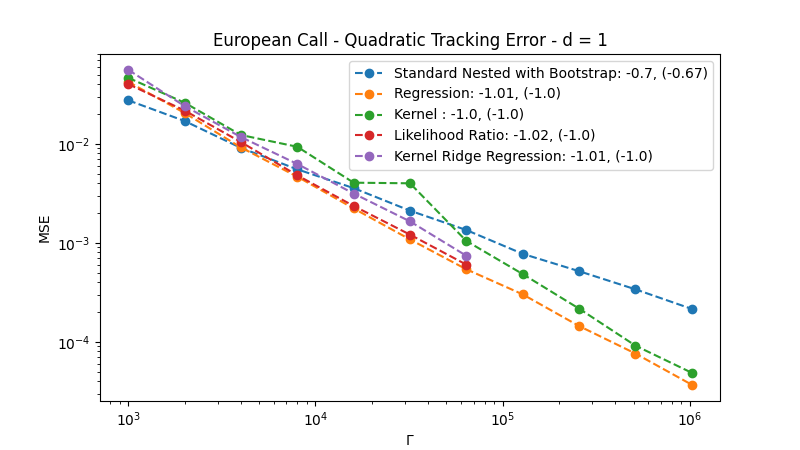
\includegraphics[width=0.7\textwidth]{./project1/figures/figure1.png}
    \caption{Empirical convergence of nested simulation procedures for quadratic tracking error on Portfolio 1 with $d=1$}
    \label{fig1:compareAll} 
\end{figure}
In Figure~\ref{fig1:compareAll}, the MSEs of the nested simulation procedures are plotted against the total simulation budget $\Gamma$ in a log-log scale, where each point represents the average MSE of the corresponding estimator over 1000 replications.
The MSEs of the nested simulation procedures are fitted with a regression line, and the slope of the fitted line is reported as the first number in the legend.
The second number in the legend is the corresponding asymptotic rate of convergence obtained from the theoretical analysis.
The slope of the fitted line can be regarded as the empirical rate of convergence of the corresponding procedure.
By comparing the empirical rates of convergence with the asymptotic rates, we can observe that the empirical rates of convergence of the standard, the kernel smoothing-based, the regression-based, the likelihood ratio-based, and the KRR-based procedures all closely match their asymptotic rates.
Due to the computational complexity of the likelihood ratio-based and the KRR-based procedures, their MSEs are not reported for $\Gamma$ larger than $16,000$ and $64,000$, respectively.
Due to the difficulty of fixing $\Gamma$ for the multi-level Monte Carlo procedure, the empirical rate of convergence of the multi-level Monte Carlo procedure is not reported here, but a detailed analysis of the empirical convergence of the multi-level Monte Carlo procedure is provided in Section~\ref{sec1:empirical-mlmc}.
In the following sections, we examine the empirical convergence of the nested simulation procedures in a similar manner as in Figure~\ref{fig1:compareAll}.
With a more detailed analysis of different risk measures, option types, and asset dimensions, we aim to provide a comprehensive understanding of the convergence behavior of the nested simulation procedures in practice.

\subsection{Sensitivity to the Asset Dimension} \label{sec1:sensitivity-dimension}
In portfolio risk management, the asset dimension is a critical factor that determines the complexity of the portfolio and the computational cost of the risk measure estimation.
The theoretical analyses in Section~\ref{sec1:convergence-orders} suggest that the asymptotic rate of convergence of the nested simulation procedures, except for the kernel smoothing-based procedure, is independent of the asset dimension.
However, the empirical convergence behavior of the nested simulation procedures could be sensitive to the asset dimension.
In this section, we examine the empirical convergence of the nested simulation procedures for different asset dimensions.

\begin{figure}[ht!]
    \centering
    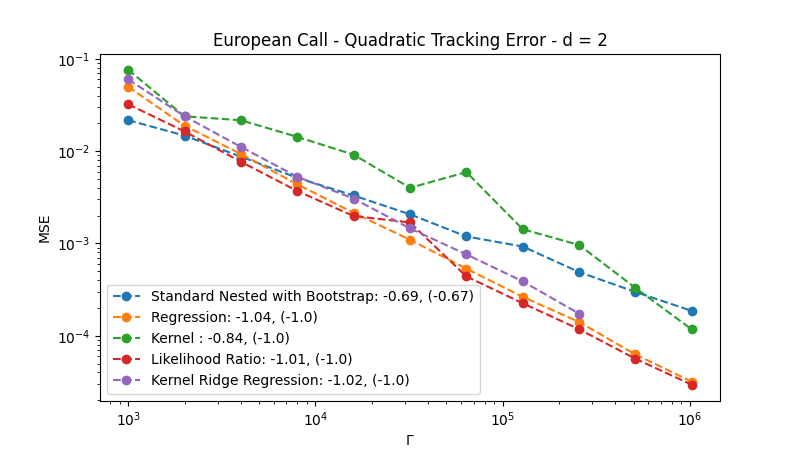
\includegraphics[width=0.48\textwidth]{./project1/figures/figure2a.png}
    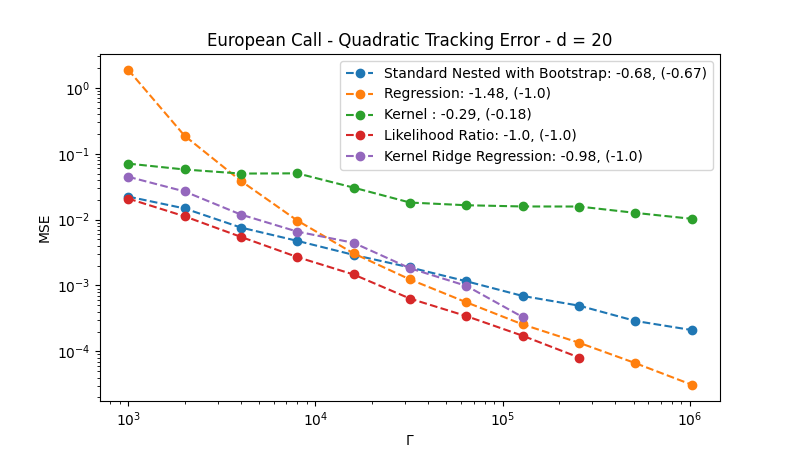
\includegraphics[width=0.48\textwidth]{./project1/figures/figure2b.png}
    \caption{Empirical convergence of nested simulation procedures for quadratic tracking error on Portfolio 1 with different asset dimensions}
    \label{fig1:assetDimension} 
\end{figure}

In Figure~\ref{fig1:assetDimension}, the empirical convergence of the nested simulation procedures for a quadratic tracking error on Portfolio 1 is illustrated for different asset dimensions, i.e., $d = 2$ and $d = 20$.
The empirical rates of convergence of the standard, the KRR-based, and the likelihood ratio-based procedures closely match their asymptotic rates for both asset dimensions, and they are independent of the asset dimension.
On the other hand, the empirical rates of convergence of the kernel smoothing-based and regression-based procedures are higher than their asymptotic rates for both asset dimensions.
They are sensitive to the asset dimension but in different ways.
The empirical rate of convergence of the kernel smoothing-based procedure decreases as the asset dimension increases.
This phenomenon is consistent with the theoretical analysis in Section~\ref{sec1:asymptotic-convergence}, where the asymptotic rate of convergence of the kernel smoothing-based procedure is shown to be sensitive to the asset dimension.
However, the empirical rate is still higher than its asymptotic rate for $d = 2$ and $d = 20$.
The empirical rates of convergence of the regression-based procedure is higher than its asymptotic rates for both asset dimensions, and the empirical rate is higher for $d = 20$ than for $d = 2$.

\subsection{Empirical Convergence of Parametric Regression Procedures} \label{sec1:regression-convergence}

For both the regression-based and the kernel smoothing-based procedures, the reason for the higher empirical rates can be explained by having poor proxy estimators for smaller simulation budgets.
For lower simulation budgets, the proxy estimators of the true inner simulation are poor, and the MSEs of the regression-based and kernel smoothing-based procedures are dominated by the model error of the proxy estimators.
In other words, they have not reached their asymptotic regimes yet.
Due to computation constraints, we are not able to conduct experiments for kernel smoothing-based nested simulation procedures for higher budget levels, but we are able to conduct additional experiments for the regression-based nested simulation procedure.
In our previous numerical experiments, the empirical rate of convergence of the regression procedure is observed to be much larger than its asymptotic rate of convergence.
For dimensions larger than 10, the MSE of the regression procedure decreases quickly in the beginning, and it stabilizes after a certain budget level.
In~\ref{fig1:reg_lb} illustrates the empirical convergence of the regression-based procedure in more detail at higher simulation budgets, where the asymptotic level of convergence is reached for $d = 20$.

\begin{figure}[ht]
    \centering
    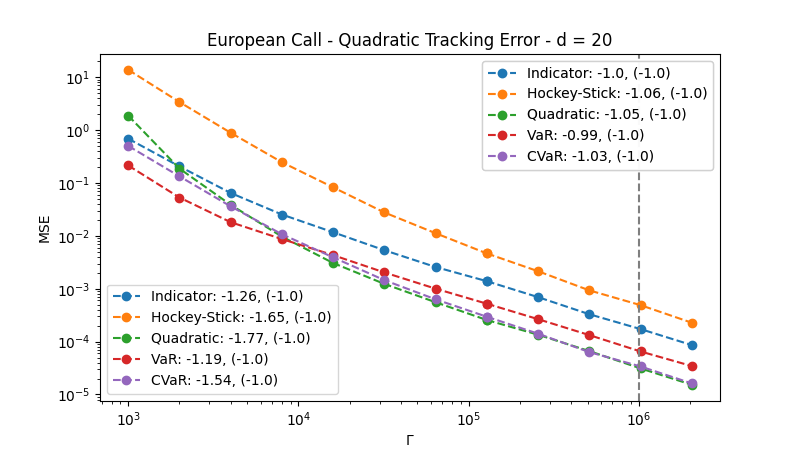
\includegraphics[width=0.7\textwidth]{./project1/figures/figure3.png}
    \caption{Empirical convergence of regression procedure for European call options and $d=20$}
    \label{fig1:reg_lb} 
\end{figure}

The left part of Figure \ref{fig1:reg_lb} contains the MSEs of the regression procedure for budget sizes that are smaller than $10,000$. 
Slopes of the fitted lines on the left correspond to the empirical rate of convergence of the regression procedure for budget levels between $1,000$ and $10,000$.
To investigate the convergence behavior for higher budget levels, we conduct additional experiments for the European call option with dimension $20$. 
The additional experiments are summarized on the right of Figure \ref{fig1:reg_lb}.
After reaching a certain budget level, i.e., $\Gamma = 1,000,000$, the empirical rate of convergence for the regression-based nested simulation procedure approaches its asymptotic rate. 
For nested simulation procedures whose proxy models are biased, the proxy estimators of the true inner simulation are poor, especially for smaller budget sizes. 
We are able to clearly observe this phenomenon for the regression proxy, and it can be explained by dividing the MSE into proxy bias and simulation variance.
For small budget sizes, the improvement of the bias of the regression proxy dominates the improvement of simulation variance. 
Performing poorly for extremely low simulation budgets, the regression proxy improves significantly. 
As the simulation budget gets higher, the improvement of the regression proxy becomes negligible compared with that of the simulation variance. 
The regression proxy ceases to improve after reaching a certain level ($\Gamma = 100\!,\!000$ in our case), and the improvement of simulation variance dominates.

\subsection{Empirical Convergence of Kernel Smoothing-Based Procedures} \label{sec1:kernel-smoothing-convergence}

The kernel smoothing proxy is a nonparametric regression procedure.
According to the theoretical analysis in Section~\ref{sec1:asymptotic-convergence}, the asymptotic rate of convergence of the kernel smoothing-based nested simulation procedure is highly dependent on the dimension of the asset.

\begin{figure}[ht!]
    \centering
    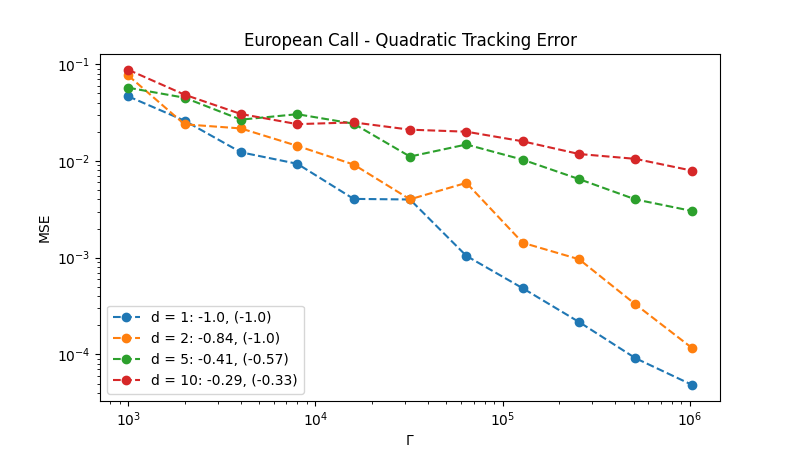
\includegraphics[width=0.48\textwidth]{./project1/figures/figure4a.png}
    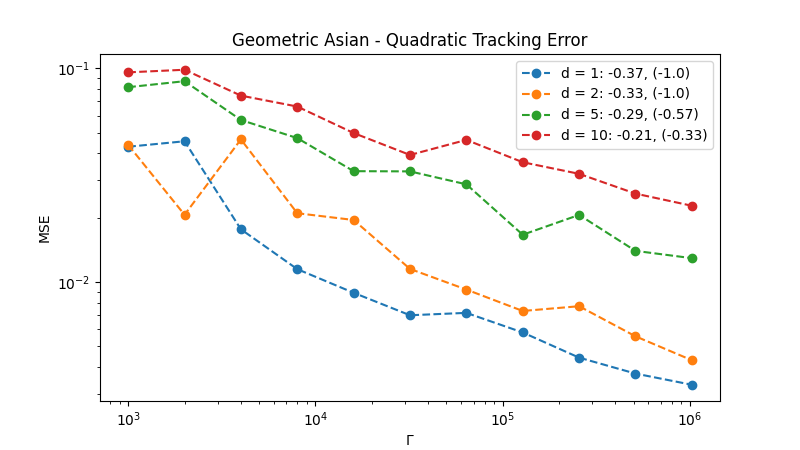
\includegraphics[width=0.48\textwidth]{./project1/figures/figure4b.png}
    \caption{Empirical convergence of kernel smoothing procedure for different values of $d$}
    \label{fig1:kernel_d} 
\end{figure}

In Figure~\ref{fig1:kernel_d}, the empirical convergence of the kernel smoothing-based nested simulation procedure for quadratic tracking error is illustrated for different asset dimensions, i.e., $d = 1, 2, 5, 10$.
The observation finds that the kernel smoothing-based nested simulation procedure is extremely sensitive to the asset dimension and the payoff structure.
While the asset dimension is expected to be a critical factor as shown in the theoretical analysis, the payoff structure is an unexpected factor that affects the empirical convergence of the kernel smoothing-based nested simulation procedure.
For a portfolio with geometric Asian options, the payoff complexity is higher than that of a portfolio with European call options.
The empirical rate of convergence of the kernel smoothing-based procedure is significantly lower for the portfolio with geometric Asian options than for the portfolio with European call options.
For geometric Asian options, the empirical rates of convergence are even lower than the asymptotic rates for all asset dimensions.

Due to the computational cost of the kernel smoothing-based nested simulation procedure, we are not able to conduct experiments for higher budget levels.
However, we are able to conduct additional experiments to examine the effects of cross-validation on the empirical convergence of the kernel smoothing-based procedure.
Another phenomenon that is observed in Figure~\ref{fig1:kernel_d} is that the empirical rate of convergence of the kernel smoothing-based procedure does not decrease monotonically as the simulation budget increases.
This is likely due to the fact that the kernel smoothing-based procedure, as a nonparametric regression procedure, is highly dependent on the cross-validation of the proxy hyperparameters.
For the kernel smoothing-based procedure, the kNN proxy is implemented. 
Hence, the proxy hyperparameter is the number of nearest neighbors $k$.
In our numerical experiment, cross-validation is conducted once to select the optimal value of $k$ for each simulation budget, and the selected value of $k$ is fixed for all $1,000$ replications.
Therefore, a poor selection of the optimal value of $k$ can lead to a poor proxy estimator, and the MSE of the kernel smoothing-based procedure will be dominated by the model error of the proxy estimator.

\begin{figure}[ht!]
    \centering
    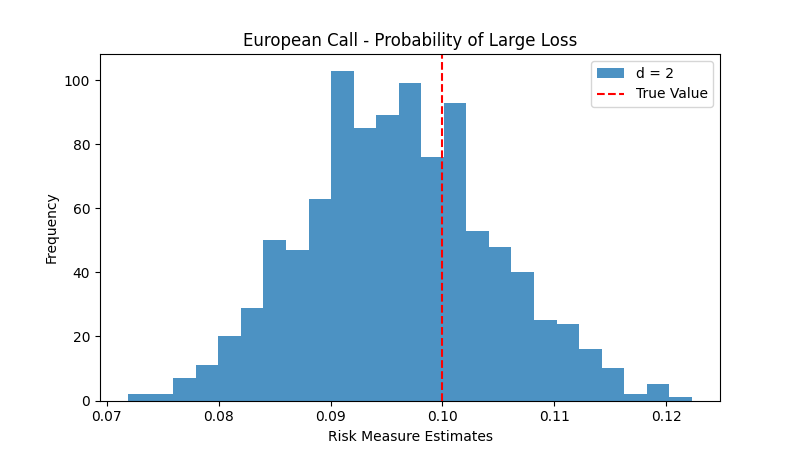
\includegraphics[width=0.48\textwidth]{./project1/figures/figure5a.png}
    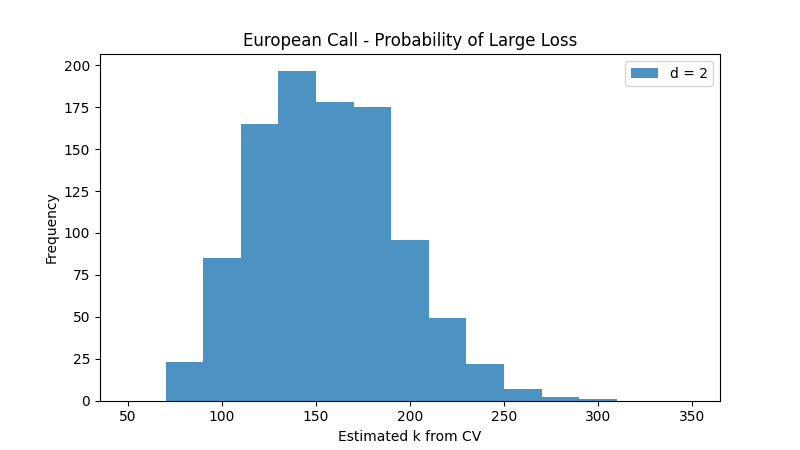
\includegraphics[width=0.48\textwidth]{./project1/figures/figure5b.png}
    \caption{Cross-validation for the kernel smoothing-based procedure with $\Gamma=100,000$}
    \label{fig1:kernel_cv} 
\end{figure}

In Figure~\ref{fig1:kernel_cv}, the empirical convergence of the kernel smoothing-based nested simulation procedure for the probability of large loss is illustrated for different values of $k$ with $\Gamma = 100,000$.
The observation is that the value of optimal $k$ estimated by cross-validation is highly variable across different replications.
For the two replications where $k = 80$ is selected as the optimal value of $k$, the estimated risk measures for the kernel smoothing-based procedure are $0.1187$ and $0.1189$, which are significantly higher than the estimated risk measures for the other replications and far from the true risk measure of $0.1$.
This observation suggests that the empirical convergence of the kernel smoothing-based nested simulation procedure is highly dependent on the cross-validation of the proxy hyperparameters.

\subsection{Sensitivity to the Option Types and Risk Measures} \label{sec1:sensitivity-option-type}

In our previous numerical experiments, we have examined the empirical convergence behavior of the nested simulation procedures for European call options, which is the most basic option type.
To examine the sensitivity of the empirical convergence behavior to the option type, we consider path-dependent options, namely geometric Asian options and barrier options.

\begin{figure}[ht!] 
    \centering
    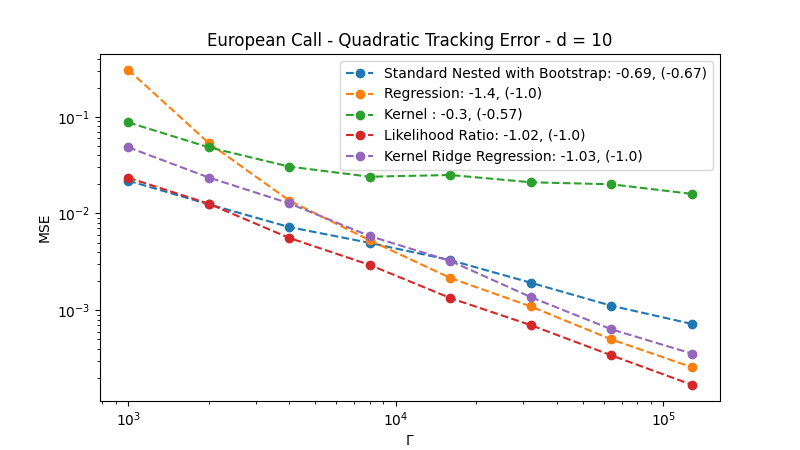
\includegraphics[width=0.48\textwidth]{./project1/figures/figure6a.png}
    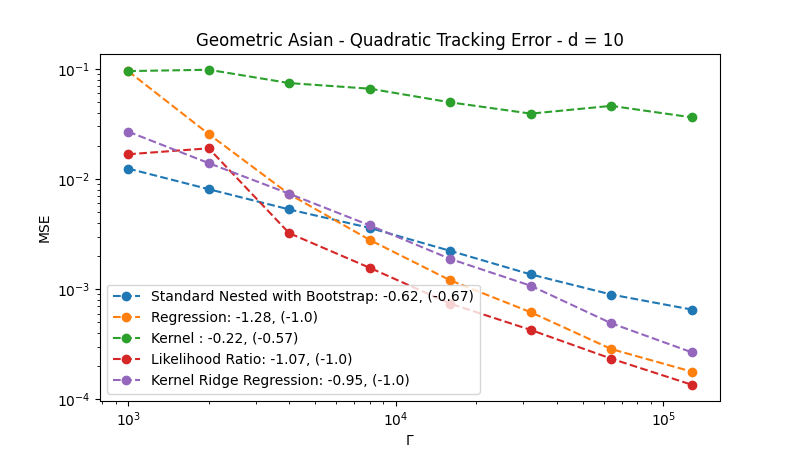
\includegraphics[width=0.48\textwidth]{./project1/figures/figure6b.png}
    \caption{Empirical convergence of nested simulation procedures for quadratic tracking error on different portfolios with $d=20$}
    \label{fig1:1x03} 
\end{figure}

In Figure~\ref{fig1:1x03}, the empirical convergence of the nested simulation procedures for the quadratic tracking errors of Portfolio 1 and Portfolio 4 is illustrated for $d = 20$.
The empirical rates of standard, likelihood ratio-based, and KRR-based nested simulation procedures closely ensemble their asymptotic rates for path-dependent options.
The empirical rate of convergence of the regression-based and kernel smoothing-based procedures is much higher than their asymptotic rates for barrier options, with reasons explained in Section~\ref{sec1:regression-convergence}.

\begin{figure}[ht!] 
    \centering
    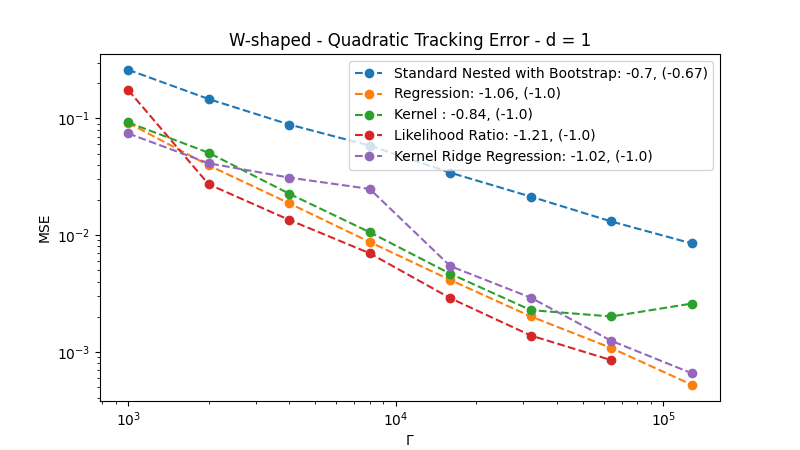
\includegraphics[width=0.48\textwidth]{./project1/figures/figure7a.png}
    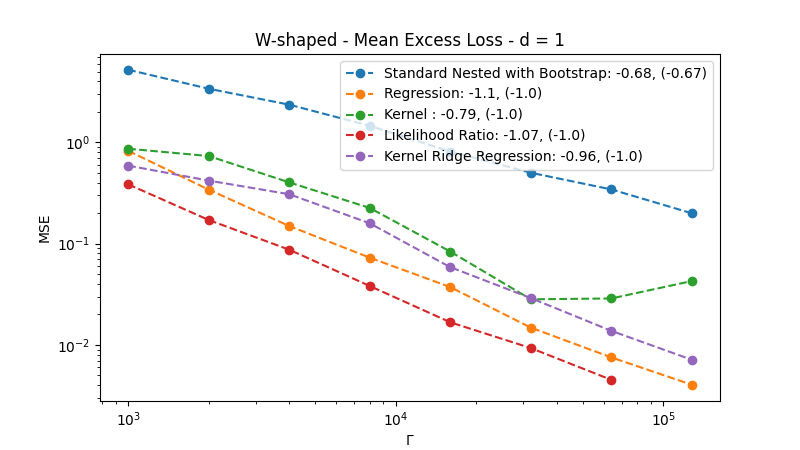
\includegraphics[width=0.48\textwidth]{./project1/figures/figure7b.png}
    \caption{Empirical convergence of nested simulation procedures for a W-shaped payoff}
    \label{fig1:5503} 
\end{figure}

In~\cite{broadie2015risk}, the authors propose a numerical example where the payoff has a W-shape with respect to the underlying asset price.
We have incorporated this example as Portfolio 5.
In Figure~\ref{fig1:5503}, the empirical convergence of the nested simulation procedures for quadratic tracking error and mean excess loss on Portfolio 5 is illustrated for $d = 1$.
For all procedures, we observe a similar convergence behavior as in other path-dependent options.
The MSEs of the kernel smoothing-based and KRR-based procedures do not decrease monotonically as the simulation budget increases, as observed and analyzed in Section~\ref{sec1:kernel-smoothing-convergence}.

\begin{figure}[ht!] 
    \centering
    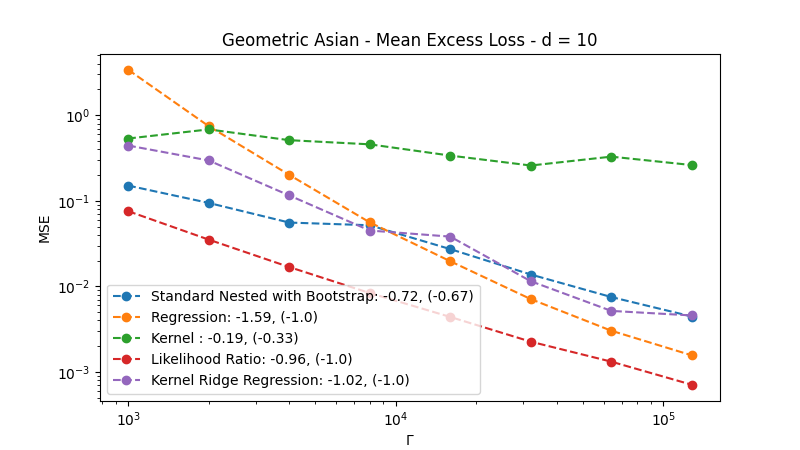
\includegraphics[width=0.48\textwidth]{./project1/figures/figure8a.png}
    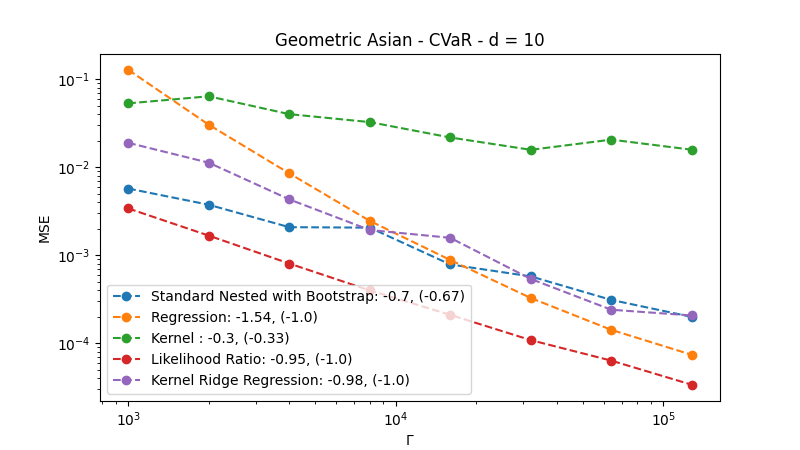
\includegraphics[width=0.48\textwidth]{./project1/figures/figure8b.png}
    \caption{Empirical convergence of nested simulation procedures for different risk measures on Portfolio 1 with $d=20$}
    \label{fig1:110x}
\end{figure}

Figure~\ref{fig1:110x} illustrates similar observations for sensitivity to different risk measures.
A change in the risk measure of interest does not affect the empirical convergence behavior of all nested simulation procedures.
From the empirical convergence results, we observe that the empirical rates of convergence of the regression-based nested simulation procedure are the highest among all nested simulation procedures for all risk measures and option types.
Furthermore, the regression-based procedure is stable across different payoff structures and risk measures. 
Its MSEs decrease quickly in the beginning, and after reaching a certain budget level, the rate of decrease stabilizes to match its asymptotic rate of convergence.

\subsection{Sensitivity to level for VaR and CVaR} \label{sec1:sensitivity-level}

The level of VaR and CVaR is a critical factor that determines the complexity of the risk measure estimation.
In our previous numerical experiments, the level of VaR and CVaR is set to be the 90\% quantile of the distribution of the inner simulation noise.
In this section, we examine the empirical convergence of the regression-based nested simulation procedures for different levels of VaR and CVaR, i.e., $80\%$, $90\%$, $95\%$, $99\%$, and $99.6\%$.

\begin{figure}[ht!] 
    \centering
    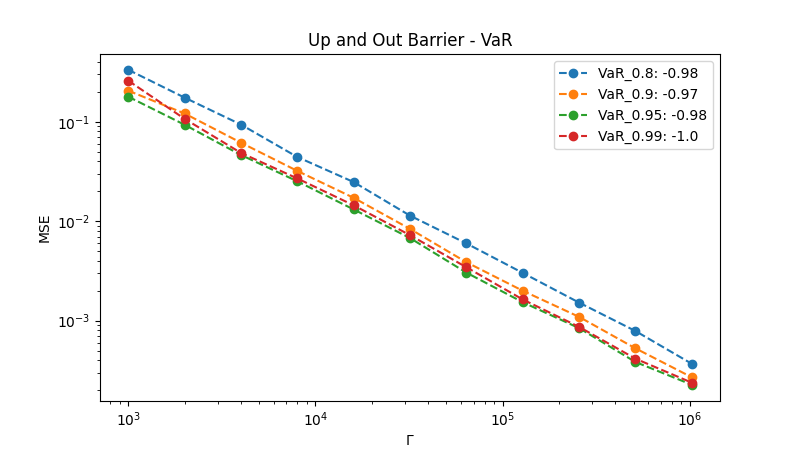
\includegraphics[width=0.48\textwidth]{./project1/figures/figure9a.png}
    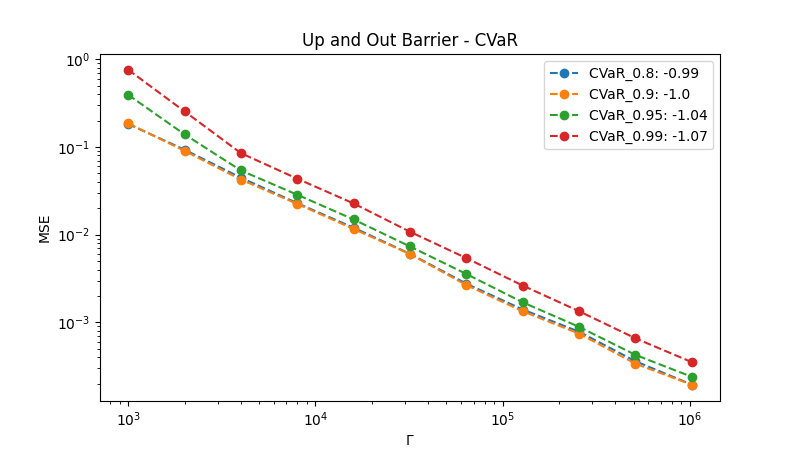
\includegraphics[width=0.48\textwidth]{./project1/figures/figure9b.png}
    \caption{Empirical convergence of regression-based procedures for different levels of VaR and CVaR for Up and Out Barrier Call Options}
    \label{fig1:sens_level}
\end{figure}

In Figure~\ref{fig1:sens_level}, the empirical convergence of the regression-based nested simulation procedure for different levels of VaR and CVaR is illustrated for up-and-out barrier call options.
The empirical rates of convergence of the regression-based nested simulation procedure are independent of the level of VaR and CVaR.

\subsection{Sensitivity to the Asset Model} \label{sec1:sensitivity-assetModel}

Our previous numerical experiments have been conducted under the assumption that the underlying asset dynamics follow a multidimensional geometric Brownian motion with $0.3$ pairwise correlation.
To examine the sensitivity of the empirical convergence behavior to the asset model, we consider a stochastic volatility model, i.e., a Heston model.

\begin{figure}[ht!] 
    \centering
    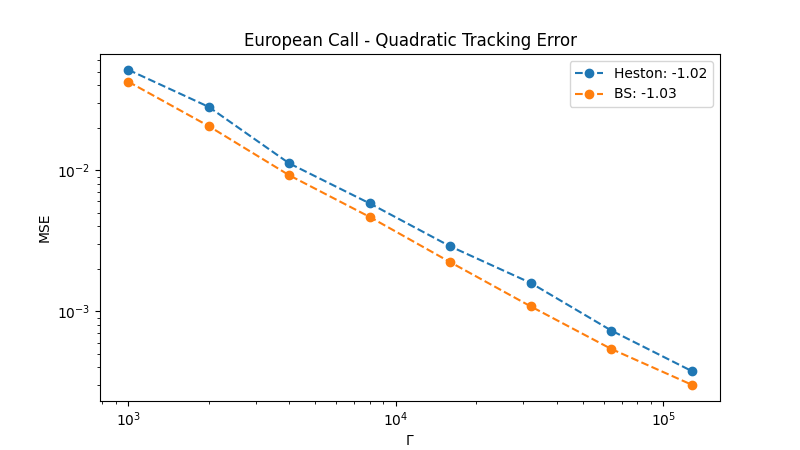
\includegraphics[width=0.48\textwidth]{./project1/figures/figure10a.png}
    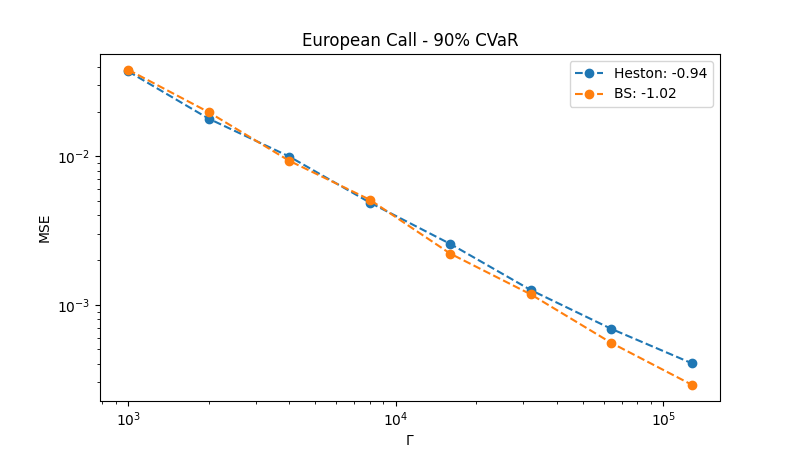
\includegraphics[width=0.48\textwidth]{./project1/figures/figure10b.png}
    \caption{Empirical convergence of regression-based nested simulation procedures for different asset models}
    \label{fig1:sens_model}
\end{figure}

In Figure~\ref{fig1:sens_model}, the empirical convergence results of the regression-based nested simulation procedure for a quadratic tracking error and a 90\%-CVaR are illustrated for different asset models, i.e., a geometric Brownian motion and a Heston model.
The empirical rates of convergence of the regression-based nested simulation procedure are observed to be independent of the asset model.

\subsection{Empirical Convergence of Multi-level Monte Carlo} \label{sec1:empirical-mlmc}

The multi-level Monte Carlo procedure is a variance reduction technique that is designed to reduce the computational cost of nested simulation procedures.
The theoretical analysis in~\cite{giles2019multilevel} shows that the multi-level Monte Carlo procedure has a faster empirical rate of convergence than the standard nested simulation procedure when the risk measure of interest is the probability of a large loss over a threshold $u$, i.e., the nested expectation case with $h$ being an indicator function.

\begin{table}[ht]
    \centering
    \begin{tabular}{rrrrrr}
    \toprule
    \textbf{Level} & \textbf{Bias} & \textbf{Variance} & \textbf{MSE} & $\Gamma$ & \textbf{MSE of SNS} \\ 
    \hline\hline
    0 & 0.118  & 0.104  & 0.1364 & 6400     & 0.1660    \\
    1 & 0.102  & 0.0916 & 0.1020 & 27600    & 0.1305    \\
    2 & 0.0870 & 0.0794 & 0.0870 & 76600    & 0.0954    \\
    3 & 0.0815 & 0.0746 & 0.0812 & 175600   & 0.0744    \\
    4 & 0.0893 & 0.0805 & 0.0884 & 348100   & 0.0460    \\
    5 & 0.0750 & 0.0694 & 0.0750 & 640000   & 0.0366    \\
    \bottomrule
    \end{tabular}
    \caption{MSEs of the multi-level Monte Carlo procedure for different levels}
    \label{tab1:mlmc-mse}
\end{table}

Instead of using a figure, we provide a summary of the empirical convergence results of the multi-level Monte Carlo procedure with a decomposition table of the MSEs in Table~\ref{tab1:mlmc-mse}.
The MSEs of the multi-level Monte Carlo procedure are decomposed into the bias and the variance of the estimator.
The MSEs of the standard nested simulation procedure with a similar total simulation budget are also provided for comparison.
Since the multi-level Monte Carlo procedure is designed with a fixed number of outer simulation paths, the benefit of the multi-level Monte Carlo procedure is minimal when the total simulation budget is large.
More specifically, when $\Gamma$ is large, the standard nested simulation procedure with a bootstrap-based budget allocation strategy benefits from having a larger number of outer simulation paths, and the MSE of the standard nested simulation procedure is lower than that of the multi-level Monte Carlo procedure with a fixed number of outer simulation paths.


\section{Computational Complexity} \label{sec1:computational-complexity}
Compared to the standard procedure, proxy-based nested simulation procedures often have faster empirical rates of convergence.
The faster convergence benefits from the pooling of inner samples through the proxy models. 
However, pooling itself comes with computational costs, which are usually ignored in most numerical comparisons. 
This section summarizes the algorithmic complexity and illustrate the computational time of different nested simulation procedures.
The findings can provide some further guidance on the choice of a proper nested simulation procedure given a nested estimation problem.
Define basic operations to be basic mathematical operators, that is, arithmetic with individual elements has complexity $\mathcal{O}(1)$.

\begin{table}[ht]
    \centering  
    \small
    \begin{tabular}{llll}
    \hline
    \textbf{Procedures}      & \textbf{Training cost}                    &  \textbf{Prediction cost}    & \textbf{Total additional cost} \\ \hline \hline
    Standard procedure       &  $0$                                      &  $\mathcal{O}(M)$            & $\mathcal{O}(M)$ \\ 
    Regression               &  $\mathcal{O}(p^2M) + \mathcal{O}(p^3)$   &  $\mathcal{O}(pM)$           & $\mathcal{O}(p^2M) + \mathcal{O}(p^3)$ \\
    Kernel smoothing         &  $\mathcal{O}(M\log(M))$                  &  $\mathcal{O}(k\log(M))$     & $\mathcal{O}(M\log(M))$ \\
    Kernel ridge regression  &  $\mathcal{O}(M^3)$                       &  $\mathcal{O}(M^2)$          & $\mathcal{O}(M^3)$ \\
    Likelihood ratio         &  $0$                                      &  $\mathcal{O}(M^2)$          & $\mathcal{O}(M^2)$ \\
    \hline
    \end{tabular} 
    \caption{Additional computational costs of nested simulation procedures aside from simulation}
    \label{tab1:complexity}
\end{table}

Table~\ref{tab1:complexity} shows the algorithmic complexity of the nested simulation procedures.
For a $d$-dimensional nested estimation problem, the simulation cost for all procedures is $\mathcal{O}(dMN)$.
The simulation cost is omitted from Table~\ref{tab1:complexity}, as all methods are given the same simulation budget.
Given $M$ outer samples and the corresponding $M$ inner sample averages, the algorithmic complexity of the additional operations does not involve $N$ thus can be written in terms of $M$ only.
The training cost includes the cost of fitting the proxy model and the cost of cross-validation for nonparametric regression proxies.
For the standard procedure, the training cost is $0$ due to the absence of proxy models. 
Its prediction cost $\mathcal{O}(M)$ comes from the evaluation of the function $h$ for $M$ samples.
For the regression-based procedure, a linear regression model is fitted with $p$ predictors.
In practice, $p$ is usually much smaller than $M$ and does not grow with the simulation budget $\Gamma$.
However, it is dependent on the complexity of the payoff function.
Estimating the coefficients of the regression model involves multiplying the design matrix by its transpose and inverting the resulting matrix, which has complexity $\mathcal{O}(p^2M)$ and $\mathcal{O}(p^3)$, respectively.
For a review in the complexity of matrix inversion, see~\cite{stothers2010complexity}.
The matrix inversion has complexity $\mathcal{O}(p^3)$ using Gauss-Jordan elimination, but in practice, the complexity can be reduced to $\mathcal{O}(p^{2.807})$ by~\cite{strassen1969gaussian} and $\mathcal{O}(p^{2.376})$ by~\cite{coppersmith1987matrix}.
The prediction cost of the regression-based procedure is $\mathcal{O}(pM)$, which comes from the multiplication of the design matrix by the estimated coefficients.
For the kernel smoothing-based procedure, the kNN proxy is implemented.
In practice, the K-D tree algorithm~\citep{bentley1975multidimensional} is often implemented for efficient nearest neighbor search.
During training, a tree is constructed to store the distance, which has complexity $\mathcal{O}(M\log(M))$.
The prediction cost of the kernel smoothing-based procedure is $\mathcal{O}(kM\log(M))$, which comes from a query of the K-D tree for $k$ nearest neighbors for $M$ samples.
Conversely, An inefficient algorithm calculates the distance matrix during training and a block sort algorithm to find the $k$ nearest neighbors, which results in a complexity of $\mathcal{O}(M^2)$ and $\mathcal{O}(M^2\log(M))$, respectively.
A practical implementation of block sort is provided in~\cite{kim2008ratio}.
Hence, an efficient implementation of the kNN proxy is crucial for the kernel smoothing-based procedure.
For the likelihood ratio-based procedure, the training cost is $0$ as no training is required.
The prediction cost of the likelihood ratio-based procedure is $\mathcal{O}(M^2)$, which comes from the calculation of the likelihood weights for $M$ samples.
For the KRR-based procedure, the main training cost comes from inverting an $M \times M$ kernel matrix~\citep{scholkopf2002learning}, which has complexity $\mathcal{O}(M^3)$ using Gauss-Jordan elimination.
Similar to the regression-based procedure, this complexity can be reduced to $\mathcal{O}(M^{2.376})$.
The prediction cost of the KRR-based procedure is $\mathcal{O}(M^2)$, which comes from the multiplication of the kernel matrix by the estimated coefficients.
Among the proxy-based procedures, regression is the most efficient as $p$ is usually much smaller than $M$. 
Kernel smoothing and KRR are kernel-based proxies, and they are more expensive due to distance calculation and cross-validation of hyperparameters. 
The kNN proxy has only 1 hyperparameter $k$, while the KRR proxy requires 3 hyperparameters, namely the smoothness hyperparameter $\nu$, scale hyperparameter $\ell$, and the regularization hyperparameter $\lambda$.
Calculating the likelihood ratio weights is inevitable for the likelihood ratio-based procedure. 
While a k-fold cross-validation is used to estimate the hyperparameter for kNN, the KRR requires Bayesian optimization~\citep{shahriari2015taking} to estimate the hyperparameters due to having a high-dimensional search space.
The likelihood ratio-based procedure requires no training, but the cost of calculating the likelihood weights is $\mathcal{O}(M^2)$.
Comparing the algorithmic complexity of the nested simulation procedures, the regression-based procedure is the most efficient among the proxy-based procedures.
For a fixed $p$, the total additional cost of a regression-based procedure is $\mathcal{O}(M)$, which is the same as the standard procedure's.


\begin{figure}[ht!]
    \centering
    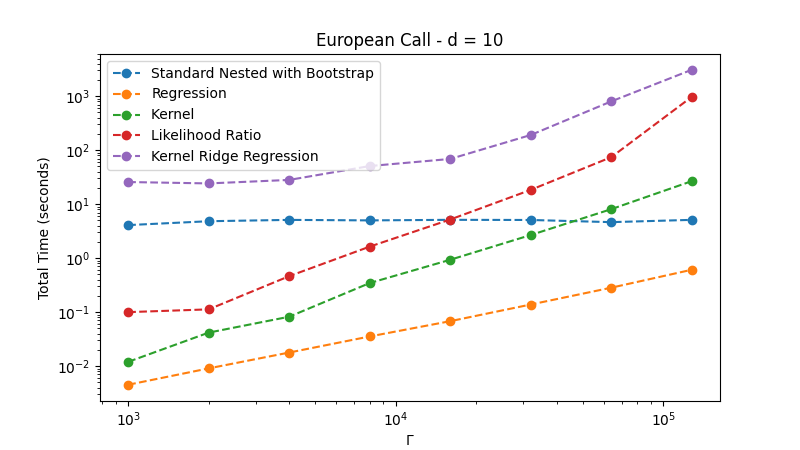
\includegraphics[width=0.48\textwidth]{./project1/figures/figure11a.png}
    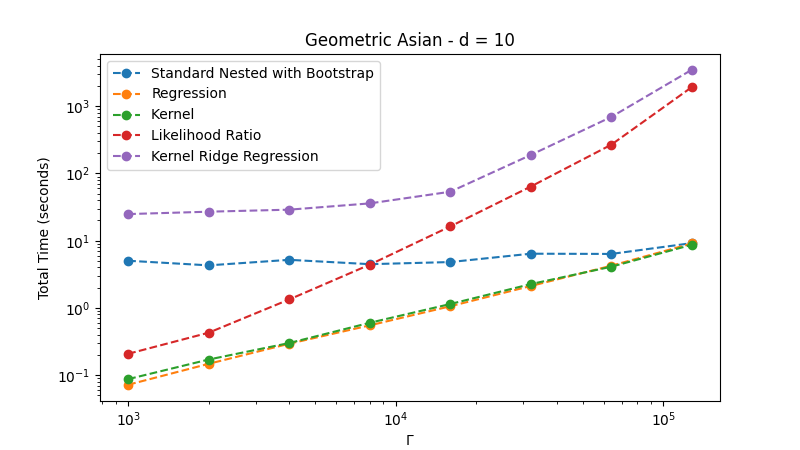
\includegraphics[width=0.48\textwidth]{./project1/figures/figure11b.png}
    \caption{Total computational cost for different procedures with $d=10$}
    \label{fig1:tcc}
\end{figure}

In our finite-sample experiments, we have observed that the actual computational cost to be significantly different from the theoretical complexity, as not only the order of complexity but also the constant factors can affect the computational cost.
In Figure~\ref{fig1:tcc}, the total computational time of different nested simulation procedures for European call options and geometric Asian options with $d = 10$ is illustrated in a log-log scale.
The $x$-axis shows the total simulation budget $\Gamma$, and the $y$-axis is the total computational time for 1 replication of the numerical experiment, in seconds.
All procedures are implemented on a machine with an AMD Ryzen 9 7900X processor with 32GB of RAM.
8 cores are used for parallel computing, and the total computational time is the sum of the simulation time, the training time, and the prediction time.
The regression and kernel smoothing-based procedures are the most efficient among the proxy-based procedures.
Since the regression-based procedure has a higher empirical rate of convergence, it is preferred over the kNN.
The likelihood ratio-based and KRR-based procedures are the most computationally expensive among all procedures.
They are demanding in terms of memory.
For budgets larger than $10^5$, the likelihood ratio-based procedure becomes impractical as storage of the likelihood weights becomes a bottleneck.
The KRR-based procedure suffers from both cross-validation and inverting a kernel matrix of size $M \times M$.
To separate the total computational time into different attributes, we provide a detailed analysis of the total computational time in the remainder of this section.

\begin{figure}[ht!]
    \centering
    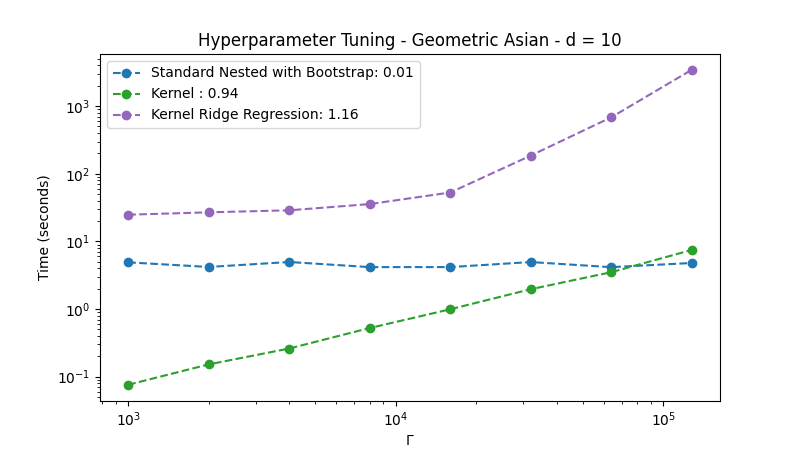
\includegraphics[width=0.48\textwidth]{./project1/figures/figure12a.png}
    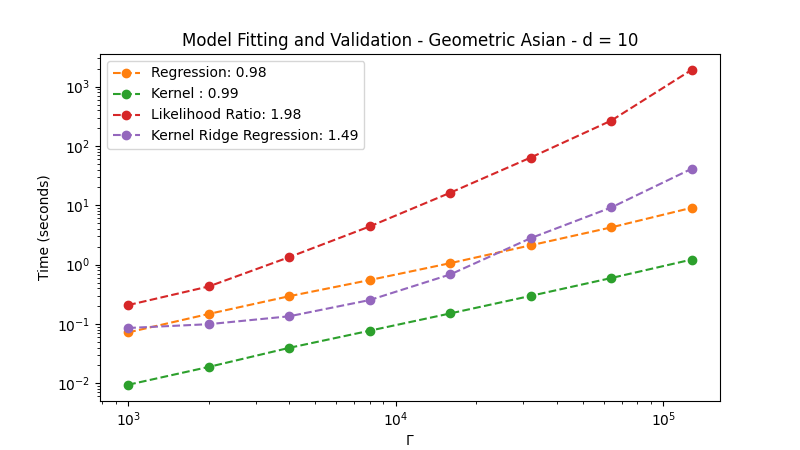
\includegraphics[width=0.48\textwidth]{./project1/figures/figure12b.png}
    \caption{Computational cost for implementing nested simulation procedures with $d=10$, excluding simulation time}
    \label{fig1:c_model}
\end{figure}

Figure~\ref{fig1:c_model} illustrates the computational time of implementing different nested simulation procedures for the portfolio of geometric Asian options with $d = 10$, excluding the simulation time.
The simulation time is omitted as it is the same for all procedures.
The remainder can be decomposed into two parts: hyperparameter tuning and model implementation.
The hyperparameter tuning cost is the cost of estimating the optimal hyperparameters for the proxy models, and the model implementation cost is the cost of fitting the proxy models and generating predictions from the trained proxies.
For each procedure, each point in Figure~\ref{fig1:c_model} represents the average computational time for a given simulation budget $\Gamma$.
A regression model is fitted to each model respectively, and its slope is reported as the growth rate of the computational time with respect to $\Gamma$.
The total computational time of the standard procedure is mostly attributed to finding the optimal $M$ and $N$ using the bootstrap-based budget allocation strategy from~\cite{zhang2021bootstrap}.
This cost does not grow with the simulation budget $\Gamma$, as its slope is close to $0$.
The regression-based procedure does not require hyperparameter tuning, and its total computational time is mainly attributed to the model implementation.
The slope of the regression line is close to $1$, resembling the its algorithmic complexity in Table~\ref{tab1:complexity}.
The kernel smoothing-based and KRR-based procedure requires cross-validation to estimate the optimal hyperparameters.
In our implementaion of kNN, the cross-validation is conducted using a grid search with a search space whose cardinality does not grow with the simulation budget $\Gamma$.
However, the cross-validation cost of the kernel smoothing-based procedure grows with the simulation budget $\Gamma$ as more samples are involved.
The KRR-based procedure requires Bayesian optimization to estimate the optimal hyperparameters, and the cardinality of the search space grows with the simulation budget $\Gamma$.
The empirical cost of the KRR-based procedure does not resemble its algorithmic complexity in Table~\ref{tab1:complexity}.
The efficient implementation of KRR is an active area of research, and the computational cost of KRR can be reduced by using a low-rank approximation of the kernel matrix, e.g., the Nystr\"om method~\citep{nystrom1930praktische}.
Our observation for KRR implementation time is in line with the findings in~\cite{scikit-learn}, where the cost of KRR is reported quickly increasing with the number of samples.
The likelihood ratio-based procedure requires no hyperparameter tuning, and its total computational time is mainly attributed to the likelihood weight calculation, which is $\mathcal{O}(M^2)$. 
In summary, for a large simulation budget, the regression-based procedure is the most efficient among all proxy-based procedures in terms of computational time.

\section{Conclusion} \label{sec1:conclusion}
In the task of estimating risk measures for portfolios of complex financial derivatives, nested simulation procedures are commonly required but often computationally expensive. 
Tremendous efforts have been made to improve the efficiency of nested simulation procedures by approximating the inner simulation model with a proxy model. 
In this study, we review the literature on nested simulation procedures in financial engineering and establish fair comparisons of different proxy models using the same set of numerical examples. 
Asymptotic properties of estimators for different nested simulation procedures are influenced by their corresponding proxy models.
To show an asymptotic convergence result, a more complex proxy model requires a more stringent set of assumptions on the distribution of the outer scenario and the inner simulation noise.
With extensive numerical experiments, we have found the finite-sample performance of a procedure can deviate from its theory. 
In theory, supervised learning-based nested simulation procedures often provide higher rates of convergence, but they come at the computational expense of model training and generating predictions from the trained models. 
The likelihood ratio-based procedure requires no training, but it is computationally expensive to compute and store the likelihood weights.
As a result, the total computational budget is not necessarily the same as the simulation budget, which is usually a limiting factor for practical applications.
A kernel-based procedure, e.g., kNN and KRR, requires cross-validation, and its empirical performance depends heavily the choice of hyperparameters.
A kNN-based procedure is sensitive to the asset dimension and the problem complexity.
A KRR-based procedure is computationally expensive, and its cost grows quickly with the simulation budget.
For kernel-based procedures, the computational cost is heavily dependent on the efficient implementation of the associated algorithms.
For a nested estimation problem with a given computational budget, we suggest the use of the regression-based simulation procedure when the budget size is moderate. 
It is efficient to implement, and it exhibits fast empirical convergence in estimating risk measures for option portfolios. 


%======================================================================
\chapter{Cutting Through the Noise: Using Deep Neural Network Metamodels for High Dimensional Nested Simulation}
\label{chap:project2}
%======================================================================


\section{Introduction}

\gls{dnn} have attracted attentions of researchers and practitioners due to their success~\citep{hastie2009elements,lecun2015deep} in solving real-world machine learning tasks such as AlphaGo~\citep{silver2016mastering} and ChatGPT~\citep{chatgpt}.
Since the first artificial neural network model~\citep{mcculloch1943logical} and the first algorithm for training a perceptron~\citep{rosenblatt1958perceptron}, especially after the introduction of backpropagation~\citep{rumelhart1985learning} and the growth of high-performance computing, the field of artificial neural network and deep learning in general has been growing rapidly.
Two specialized neural network architectures that are relevant to our study are \gls{rnn}~\citep{williams1989learning,sutskever2014sequence} and \gls{lstm}~\citep{hochreiter1997long,chung2014empirical}.
In the field of actuarial science, a metamodel is commonly referred to as a proxy model.
Despite their success, \gls{dnn} models are often criticized for their lack of transparency and interpretability, which hinders their adoption in financial and actuarial applications.
Enormous research efforts have been spent to test and improve the robustness of \gls{dnn} models with carefully designed noise injection methods.
~\cite{poole2014analyzing} show that injecting synthetic noise before and after hidden unit activations during training improves the performance of autoencoders.
~\cite{neelakantan2015adding} improve learning for \gls{dnn}s by injecting synthetic noise to the gradients during backpropagations.
A branch of research has been devoted to understanding the resilience of neural network models to noise in training labels.
For example,~\cite{luo2016understanding} show that adding synthetic label noise to the convolutional neural network (\gls{cnn}) can improve its ability to capture global features. 
~\cite{srivastava2014dropout} quantify the error tolerance by injecting synthetic label noise with a custom Boltzmann machine hardware.
~\cite{szegedy2013intriguing} find that neural networks are vulnerable to adversarial examples, and~\cite{goodfellow2014explaining} design an efficient method to generate such noisy examples to exploit the vulnerability to adversarial perturbations.
~\cite{carlini2017towards} design targeted attacks to training labels to test the robustness of neural networks. 
Instead of using synthetic noise, ~\cite{jiang2020beyond} inject real-world label noise and examine noise tolerance of neural networks with controlled noise levels.
The aforementioned studies use real-world data, as is typically the case for many neural network studies, where noise is already present in the training labels before any noise injection.
Users of real-world data have little control over the noise level of the original training labels and usually examine the effect of noisy data by injecting noise, but it is unclear whether a neural network model trained on noisy data actually learns the real, i.e., noiseless, feature-label relationship.
Due to their lack of transparency and interpretability, the adoption of \gls{dnn}s in financial and actuarial applications has been received by regulators with some skepticism.

The contributions of our study in this chapter are two-fold:
\begin{enumerate}
    \item We study what \gls{dnn}s learn from noisy data by training them using simulated data based on well-designed simulation experiments.
    This is a novel way to study the effect of noisy data and error tolerance of neural network models as one can \textit{reduce noise} in the data by increasing the number of replications in a simulation model.
    This new way of studying neural network models can provide more direct evidence on their transparency and interpretability. 
    \item We propose two generic nested simulation procedures that uses \gls{dnn}s as metamodels to improve its efficiency while maintaining transparency. 
    In essence, a pilot stage simulation is used to generate a large number of noisy data, which are then used to train a metamodel.
    Depending on the application, a trained metamodel can serve two purposes: 
    \begin{itemize}
        \item to identify a set of tail scenarios, and 
        \item to estimate risk measures directly.
    \end{itemize}
    The first procedure uses a metamodel to identify a set of potential tail scenarios on which computations are performed in stage 2, while the second procedure uses metamodel predictions to estimate risk measures directly.
    Our numerical results show that \gls{dnn} metamodels can identify the tail scenarios accurately and so the proposed procedures can estimate tail risk measures with a similar degree of accuracy while, at the same time, using less simulation budget.
\end{enumerate}

In essence, we are curious about two fundamental questions:
\begin{enumerate}
    \item ``What do \gls{dnn}s learn from noisy data?'' and 
    \item ``How well do neural networks learn from noisy data?''.
\end{enumerate}
Data-driven answers to these questions prevail in the existing literature.
In supervised learning, \gls{dnn}s are believed to learn from a given data about the feature-label relationship to predict new labels for unseen features.
A cross-validation procedure used to assess a subset, i.e., the validation set, of the original data, is a common way to access the quality of learning.
Generalization error on the test labels is another popular assessment metric.
However, the test set is also a subset of the original data.
In this study, we revisit these questions in a simulation context and propose an alternative approach to answer them.
Instead of relying solely on real-data and splitting it into multiple subsets, we propose using stochastic simulation outputs as training labels for \gls{dnn}s.
By controlling the simulation design parameters, such as the number of independent replications, we can control the quality and also the quantity of the training labels fed into the neural networks.
In such a controlled environment, we obtain more clear-cut answers to the above fundamental questions.

In a nested simulation, a simulation model is used to generate a large number of outer scenarios, and each scenario is then used as an input to another simulation model, referred to as an inner simulation model.
Borrowing terminologies from the machine learning community, we can view a set of simulated outer scenarios and estimated hedging errors for those scenarios as \textit{features} and noisy \textit{labels}.
The noise level of the labels can be controlled by the number of inner replications in the inner simulation model.
One can train supervised learning models using these simulated features and labels.
They are then used to replace the time-consuming inner simulations by the trained model.
We refer to the trained supervised learning models as \textit{metamodels} of the inner simulation, which is also known as the \textit{surrogate models} in the simulation literature.
Metamodeling is a popular approach to reduce the computational burden of simulation-based applications by replacing the time-consuming simulation with a metamodel.
The metamodel is trained using a set of simulated data, and it is used to predict the simulation output for new inputs.
The study of metamodeling is an active research area in the simulation literature, and using \gls{dnn}s as metamodels is a relatively new development.
~\cite{fonseca2003simulation} provide general guidelines for simulation metamodeling with neural networks,~\cite{lieu2022adaptive} use \gls{dnn}s as metamodels of a simulation model for a structural reliability analysis, and~\cite{salle2014efficient} show that neural network metamodels help achieve higher degree of prediction accuracy that other metamodels in approximating agent-based simulation models.
A popular metamodel in nested simulation procedures is stochastic kriging.
~\cite{liu2010stochastic} use stochastic kriging as a metamodel of Monte Carlo simulations to estimate the \gls{cvar} of a portfolio of derivative securities, and~\cite{gan2015valuation} use a stochastic kriging for an efficient valuation of large portfolios of \gls{va} contracts.
Other studies, such as ~\cite{broadie2015risk},~\cite{hong2017kernel}, and~\cite{zhang2022sample} use a regression, a kernel smoothing, and a likelihood ratio method, respectively as metamodels.
Our study has three key distinctions over the existing ones:
\begin{enumerate}
    \item  our metamodel has high-dimensional inputs. In machine learning terminology, the features are high-dimensional vectors.
    To estimate the hedging error of a typical \gls{va} contract, the number of features is in the order of hundreds, which is at least one order of magnitude larger than the number of features in the aforementioned studies,
    \item  for estimating tail risk measures, our metamodel is only used for tail scenario identification but is \textit{not} used in the estimation of the tail risk measures.
    This is a feature designed particularly to convince regulators that the losses used in estimating the risk measure are based on a transparent inner simulation model rather than on some black-box metamodels, and
    \item  using simulation models as data generators, we can decrease the noise level and get arbitrarily close to the true labels by increasing the number of replications in the simulation model.
    This design allows a systematic study of the effect of noisy training labels on the performance of \gls{dnn} models in predicting the noiseless labels.
\end{enumerate}

In this chapter, \gls{dnn} metamodels and \gls{dnn} models are used almost interchangeably despite one distinction.
\begin{itemize}
    \item The discussion of \textit{\gls{dnn} metamodels} focuses more on the aspect of \textit{estimating} the inner simulation.
    \item The discussion of \textit{\gls{dnn} models} focuses more on \textit{studying the \gls{dnn}} using simulation data.
\end{itemize}

The rest of this chapter is organized as follows.
Section~\ref{sec2:problem-formulation} presents the problem settings for tail risk measures and dynamic hedging of \gls{va}s. 
Section~\ref{sec2:metamodel2Stage} proposes an efficient two-stage nested simulation procedure that uses \gls{dnn}s as metamodels to help reduce a simulation budget by only performing computations on identified tail scenarios. 
Section~\ref{sec2:metamodel1Stage} proposes a single-stage nested simulation procedure that estimates risk measures directly with metamodel predictions.
Section~\ref{sec2:numerical} demonstrates the efficiency of \gls{dnn} metamodels and examines the error tolerance of two \gls{lstm} metamodels with different numbers of trainable parameters. 
Lastly, practical suggestions are provided for the choice of suitable metamodels and simulation settings. 

\section{Problem Formulation} \label{sec2:problem-formulation}

In this section we present notations, problem settings, and a simulation model for risk estimation for hedging errors of \gls{va}s.
A main goal of this section is to showcase the complexity of the simulation model, which we use as a data generator to train \gls{dnn} metamodels (Section~\ref{sec2:metamodel2Stage} and Section~\ref{sec2:metamodel1Stage}).
For readers who are interested in the examination of a neural network metamodel, it is sufficient to understand that our simulation model generates data with 240 features and 1 real-value label and our metamodels are generally applicable to any simulation model that generates data with similar characteristics.

\subsection{Tail Risk Measures}
Measuring and monitoring risks, particularly tail risks, are important risk management tasks for financial institutions such as banks and insurance companies.
Two most popular tail risk measures are \gls{var} and \gls{cvar}~\citep{hardy2022quantitative, rockafellar2002conditional}. 

Consider a loss random variable $L$ which losses and gains lie in the right and left tails, respectively, of its distribution.
For a given confidence level $\alpha\in [0,1]$, the $\alpha$-\gls{var} and $\alpha$-\gls{cvar} are defined in Equation~\eqref{eq1:var} and Equation~\eqref{eq1:cvar}, respectively.
Tail risk measures such as \gls{var} and \gls{cvar} are widely used for setting a regulatory and economic capital, which is the amount of capital a financial institution holds to cover its risk.
For example, European insurers set regulatory capital at $99.5\%$-\gls{var} according to Solvency II~\cite{eiopa2014underlying}.
In Canada, the regulatory capital requirement for \gls{va}s is set based on \gls{cvar}s as prescribed in~\cite{osfi2017life}.

Let $L_1,L_2,\ldots,L_M$ be $M$ i.i.d. simulated losses of $L$ and let $L_{(1)}\leq L_{(2)}\leq \ldots\leq L_{(M)}$ be the ordered losses.
For a given confidence level $\alpha$ (assume that $\alpha M$ is an integer for simplicity), $\alpha$-\gls{var} can be estimated by the sample quantile $\widehat{\VaR}_\alpha = L_{(\alpha M)}$. Also, $\alpha$-\gls{cvar} can be estimated by
\begin{equation} \label{eq2:cvar-hat}
    \widehat{\CVaR}_\alpha = \frac{1}{(1-\alpha)M} \sum_{i=\alpha M + 1}^{M}L_{(i)} = \frac{1}{(1-\alpha)M} \sum_{i \in \tail_{(1-\alpha )M}}L_{i}.
\end{equation}

Equation \eqref{eq2:cvar-hat} is the same as \eqref{eq1:cvar-hat} except that we define a \textit{true tail scenario set} of size $k$ as $\tail_{k} = \{i: L_i > L_{(M-k)}\}$.
In this study, the loss random variable of interest is the hedging error for \gls{va}.

\subsection{Simulation Model for Variable Annuity Payouts}\label{subsec:VApayout}

\gls{va} contracts offer different types of guarantees.
Generally speaking, a portion of the \gls{va} premium is invested in a sub-account which return is linked to some stock indices.

Two relevant types of guarantees in our studies are:
\begin{itemize}[noitemsep]
    \item \textbf{\gls{gmmb}}: A \gls{gmmb} contract pays a maturity benefit equal to the greater of the sub-account value and a fixed guarantee value.
    The guarantee value is often set as a percentage, e.g., 75\% or 100\%, of the initial premium.

    \item \textbf{\gls{gmwb}}: A \gls{gmwb} contract guarantees the minimum amount of periodic withdrawal the policyholder can take from the sub-account until maturity, even if the sub-account value reduces to zero.
    The minimum withdrawal benefit is typically a fixed percentage of the guarantee value.
    The guarantee value will decrease if the withdrawal exceeds the guaranteed minimum. The \gls{gmwb} is typically offered with an accumulation period, during which no withdrawals are made but a \gls{gmab} is usually offered. Additional features offered with the \gls{gmwb} include roll-up, ratchet, and reset~\citep{geneva2013variable}.
\end{itemize}
For a comprehensive review of other types of \gls{va} contracts such as \gls{gmab}, \gls{gmdb}, and \gls{glwb}, we refer readers to~\cite{hardy2003investment}.
Next we present a summary of dynamic hedging for \gls{va} contracts.
We refer readers to~\cite{dang2021efficient} for detailed modeling of insurer liabilities in different \gls{va} contracts and Greek estimation.

Consider a generic \gls{va} contract with maturity $T>0$ periods, e.g., $T=240$ months.
Denote the policyholder's (random) time of death by $\tau>0$.
The contract expires at $T'=\min\{T,\tau\}$, which isthe earlier of the contract maturity and the death of the policyholder.
Let $S_t$, $F_t$, and $G_t$ be an indexed stock price, the subaccount value and a guarantee value, respectively, at time $t=1,2,\ldots,T$.
Evolution of the subaccount value and the guarantee value of a \gls{va} contract affect the contract payout.
Let the triplet $X_t = (S_t, F_t, G_t)$ be the state of the \gls{va} contract at time $t$.
Note that the policyholder's (random) time of death also affects the timing of the benefit payout for certain types of \gls{va} such as \gls{gmab}, but this is not considered in our study for simplicity.
For clarity, we use $F_t$ and $F_{t_+}$ to denote the sub-account value just before and just after the withdrawal at time $t$, if any.
Let $\eta_g$ be a gross rate of management fee that is deducted from the fund value at each period and let $\eta_n < \eta_g$ be a net rate of management fee income to the insurer.
The difference between the gross management fee and the net management fee income represents incurred investment expenses.

At the inception of the contract, i.e., $t=0$, we assume that the whole premium is invested in the stock index and the guarantee base is set to the sub-account value:
\begin{equation*}
    S_0=F_0=G_0.
\end{equation*}
At each time $t=1,\ldots,T$, the following events take place in order:
\begin{enumerate}
    \item The sub-account value changes according to the growth of the underlying stock and the (gross) management fee is deducted, which is, 
        \begin{equation*}
            F_t = F_{(t-1)_+}\cdot\frac{S_{t}}{S_{t-1}}\cdot(1-\eta_g),
        \end{equation*} 
    where $(x)^+=\max\{x,0\}$ and $F_{(t-1)_+}$ will be defined later. The insurer's income at time $t$ is a net management fee, i.e., $F_t\eta_n$. 

    \item The guarantee value ratchets up (ratcheting is a common feature in \gls{gmwb}) if the sub-account value exceeds the previous guarantee value,
        \begin{equation*}
            G_t = \max\{G_{t-1},F_t\}.
        \end{equation*} 

    \item The withdrawal is made (for \gls{gmwb}) and is deducted from the sub-account value,
        \begin{equation*}
            F_{t_+} = (F_t - I_t)^+,
        \end{equation*} 
    where $I_t = \gamma G_t$. A \gls{gmmb} can be modeled with $\gamma = 0$.
\end{enumerate}

We see from the above modeling steps that the status of a generic \gls{va} contract is summarized by a triplet $(S_t,F_t,G_t)$ which evolution is driven by the stochasticity of $S_t$.
In practice, the simulation model may also incorporate additional complications such as mortality, lapse, and excess withdrawal, etc.

At any time $t=1,\ldots,T$, the insurer's liability in a \gls{va} contract is the present value of all payments, net of the fee income.
For example, suppose that the per-period risk-free rate is $r$, then
\textcolor{red}{the insurer's time-$t$ liability for a \gls{gmwb} contract is}

\begin{equation} \label{eq2:liability-gmwb}
    V_t = V(\mathbf{S}_t) = \mathbb{E} \left[ e^{-r(T-t)}\cdot (G_T - F_T)^+ - \sum_{s=t+1}^{T} e^{-r(T-s)} F_s \eta_n \big\vert \mathbf{S}_t \right],
\end{equation}

where $\mathbf{S}_t = (S_0, S_1, \ldots, S_t)$ is the (outer) sample path up to time $t$, and the conditional expectation is taken with respect to the inner sample paths $\Stilde_{t+1},\ldots,\Stilde_{T}$ given the outer path $\mathbf{S}_t$.
The tilde symbol ($\sim$) over a quantity denotes its association with the inner simulation.
In practice, given the stock sample path, which is an outer path $S_1,\ldots,S_t$, one can simulate these future stock prices $\Stilde_{t+1},\ldots,\Stilde_{T}$ with an inner simulation model that is based on some asset model such as \gls{gbm} or \gls{rsgbm}.
Given the time~$t$ state $(S_t,F_t,G_t)$, following~\cite{cathcart2015calculating} the sensitivity of $V_t$ with respect to $S_t$ can be estimated by a pathwise estimator~\citep{glasserman2004monte}:
\begin{align}\label{eq2:delta}
    \Delta_t(\Stilde_{t+1},\ldots,\Stilde_{T} | \mathbf{S}_t) 
    & = \frac{\partial V_t}{\partial S_t} \nonumber \\
    & = \frac{\partial}{\partial S_t} \mathbb{E} \left[ e^{-r(T-t)}\cdot (G_T - F_T)^+ - \sum_{s=t+1}^{T} e^{-r(T-s)} F_s \eta_n \big\vert \mathbf{S}_t \right] \nonumber \\
    & = \mathbb{E} \left[ \frac{\partial}{\partial S_t} \left( e^{-r(T-t)}\cdot (G_T - F_T)^+ - \sum_{s=t+1}^{T} e^{-r(T-s)} F_s \eta_n \right) \big\vert \mathbf{S}_t \right] 
\end{align}

For an inner simulation path $\Stilde_{t+1},\ldots,\Stilde_{T}$ of the \gls{gmwb} contract, the sensitivity of $V_t$ can be calculated by the following recursion:
\begin{equation}
    \sum_{s=t+1}^{T} e^{-r(T-s)} \left[\bm{1}\{\Itilde_{t,s} > \Ftilde_{t,s}\} \cdot \left( \frac{\partial \Itilde_{t,s}}{ \partial S_t} - \frac{\partial \Ftilde_{t,s}}{ \partial S_t}\right)- \eta_n \frac{\partial \Ftilde_{t,s}}{ \partial S_t}\right], \nonumber \\
    t=0,\ldots,T-1, 
\end{equation}
where $\bm{1}\{\cdot\}$ is an indicator function, $\Stilde_t = (S_{t, t+1},\ldots,S_{t, T})$, $\Ftilde_t = (F_{t, t+1},\ldots,F_{t, T})$, $\Gtilde_t = (G_{t, t+1},\ldots,G_{t, T})$, $\Itilde_t = (I_{t, t+1},\ldots,I_{t, T})$, and
\begin{align} \label{eq2:partial-derivatives}
    \frac{\partial \Ftilde_{t, s}}{ \partial S_t} &= \bm{1}\{\Itilde_{t, s-1} < \Ftilde_{t, s-1}\}\cdot\left( \frac{\partial \Ftilde_{t, s-1}}{ \partial S_t} - \frac{\partial \Itilde_{t, s-1}}{ \partial S_t}\right) \cdot \frac{\Stilde_{t, s}}{\Stilde_{t, s-1}}\cdot (1-\eta_g),\nonumber \\
    \frac{\partial \Gtilde_{t, s}}{ \partial S_t} &= \bm{1}\{\Gtilde_{t, s-1} < \Ftilde_{t, s}\}\cdot\frac{\partial \Ftilde_{t, s}}{ \partial S_t} + \bm{1}\{\Gtilde_{t, s-1} \geq \Ftilde_{t, s}\}\cdot\frac{\partial \Gtilde_{t, s-1}}{ \partial S_t},\nonumber \\
    \frac{\partial \Itilde_{t, s}}{ \partial S_t} &= \gamma \frac{\partial \Gtilde_{t, s}}{ \partial S_t}.
\end{align}
At each inner simulation, the sample path at $t$ is initialized as:
\begin{equation}
    (\tilde{X}_{t, t}) = (\tilde{S}_{t, t}, \tilde{F}_{t, t}, \tilde{G}_{t, t}) = (S_t, F_t, G_t) = (X_t)
\end{equation}
Before withdrawal at $t$, the partial derivatives are initialized. $\tilde{F}_{t, t}$ is set to be proportional to $\tilde{S}_{t}$, such that:
\begin{equation}
    \frac{\partial \Ftilde_{t, t}}{ \partial S_t} = \frac{\partial F_t}{ \partial S_t} = \frac{F_t}{S_t},
\end{equation}
and $\tilde{G}_{t, t}$ and $\tilde{I}_{t, t}$ are fixed as constants, such that:
\begin{equation}
    \frac{\partial \Gtilde_{t, t}}{ \partial S_t} = \frac{\partial G_{t}}{ \partial S_t} = 0, \quad \frac{\partial \Itilde_{t, t}}{ \partial S_t} = \gamma \frac{\partial I_{t}}{ \partial S_t} = 0.
\end{equation}
Note that in Equation~\ref{eq2:partial-derivatives}, no calculation is needed for $F_t \leq I_t$. 
In this case, the sub-account is already depleted at time $t$ and withdrawals are not allowed.
Therefore, \gls{gmwb}'s future liabilities beyond time $t$ are no longer affected by the stock price $S_t$, so no hedging is necessary.
In other words, when $F_t < I_t$, the inner simulation can be skipped and set $\Delta_t = 0$.

\subsection{Dynamic Hedging for Variable Annuities}\label{subsec:dynamicHedge}

Below we provide a scheme used to perform a multi-period nested simulation in estimating \gls{pl} for one outer scenario.

\begin{figure}[ht]
    \centering
    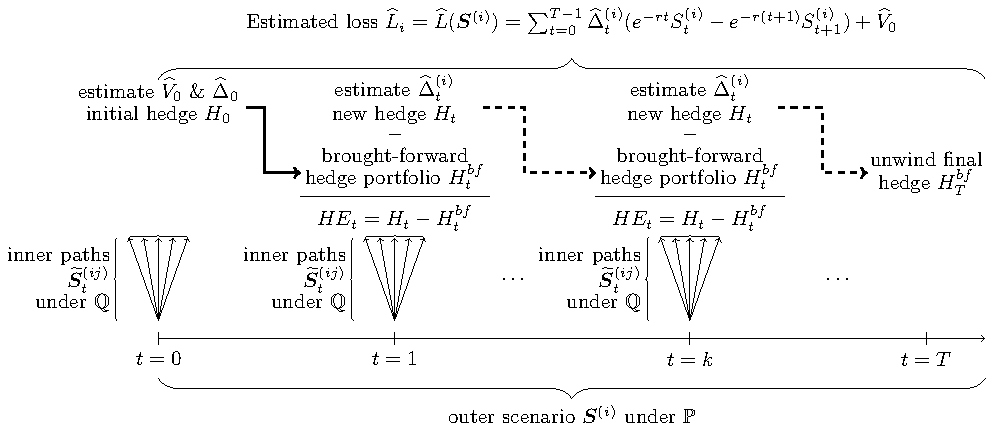
\includegraphics[width=0.85\textwidth]{./project2/figures/sns.pdf}
    \caption{Illustration of a multi-period nested simulation that estimates the P\&L for one outer scenario.}
    \label{fig2:illustration}
\end{figure}

Insurers commonly use dynamic hedging to mitigate a market risk exposure in \gls{va} contract's embedded options.
In a dynamic hedging program, a hedge portfolio is set up and periodically rebalanced for a portfolio of \gls{va} contracts using stocks, bonds, futures, and other derivatives.
For simplicity, in this study we consider delta hedging for a generic \gls{va} liability using one stock and one bond.
The metamodeling procedures presented in Section~\ref{sec2:metamodel2Stage} and Section~\ref{sec2:metamodel1Stage} can be trivially adapted to more general hedging strategies.

Consider hedging a \gls{va} contract whose sub-account is invested in a stock, and the hedging portfolio is rebalanced monthly.
At $t \leq T$, a dynamic equation can be specified for the sub-account value $F_t$, in the absence of withdrawals, as:
\begin{equation*}
    F_t = F_{t-1} \cdot \frac{S_t}{S_{t-1}} \cdot (1-\eta_g)
\end{equation*}
where $\eta_g> \eta_n$ is the gross rate of management fee that is deducted from the sub-account value at the end of each month.
The delta hedge portfolio at any month~$t$, $t=0,1,\ldots,T-1$, consists of $\Delta_t$ units in the underlying stock and $B_t$ amount of a risk-free zero-coupon bond maturing at $T$ months.
The value of the hedge portfolio at month~$(t-1)$ is:
\begin{equation*}
    H_{t-1} = \Delta_{t-1} S_{t-1} + B_{t-1},
\end{equation*}
where $S_t$ is an underlying stock price and any month $t>0$.
Assuming there is no rebalacing between $t-1$ and $t$, this hedge portfolio is brought forward to month~$t$,.
Its value at month~$t$ becomes:
\begin{equation*}
    H_{t}^{bf} = \Delta_{t-1} S_{t} + B_{t-1}e^{-rt}.
\end{equation*}
Therefore, the time~$t$ hedging error, which is the cash flow incurred by the insurer due to rebalancing at time~$t$, is
\begin{equation}\label{eq2:hedgingerror}
    HE_t = H_t - H^{bf}_t, \quad t=1,\ldots, T-1.
\end{equation}
The \gls{pl} of the \gls{va} contract includes cost of the initial hedge ($H_0$), hedging errors~\eqref{eq2:hedgingerror}, unwinding of the hedge at maturity ($H^{bf}_T$), and unhedged liability ($V_0$).
Mathematically, the present value of these cash flows is given by
\begin{equation}\label{eq2:lossrv}
L = H_0 + \sum_{t=1}^{T-1} e^{-rt} HE_t - e^{-rT} H^{bf}_T + V_0 = \sum_{t=0}^{T-1}\Delta_t (e^{-rt}S_t - e^{-r(t+1)}S_{t+1}) + V_0,
\end{equation}
where the second equality holds by a telescopic sum simplification of $e^{-rt}B_t$, $t=0,\ldots,T-1$.

In~\eqref{eq2:lossrv}, $\Delta_t$ and $V_0$ are determined by using a risk-neutral measure $\mathbb{Q}$ while the distribution of $L$ is under a real-world measure $\mathbb{P}$.
If $\Delta_t$ and $V_0$ cannot be calculated analytically, a nested simulation is required to estimate the tail risk measure of $L$.
Recall from Section~\ref{subsec:VApayout} that the stock sample path, regardless of the inner or outer simulation or a combination of both, determines the evolution of the triplet $(S_t,F_t,G_t)$.
Specifically, the outer scenarios $\bS^{(i)} = (S_{1}^{(i)},\ldots,S_{T}^{(i)})$, $i=1,\ldots,M$ are generated under $\mathbb{P}$.
At each time~$t=1,\ldots,T-1$ of a given outer scenario $\bS^{(i)}$, inner sample paths $\bStilde_{t}^{(j)} = (\Stilde_{t+1}^{(j)},\ldots,\Stilde_{T}^{(j)})$, $j=1,\ldots,N$ are generated under $\mathbb{Q}$ to estimate $\Delta_t^{(i)}$, $i=1,\ldots,M$.
Also, $V_0^{(i)}$, $i=1,\ldots,M$ are estimated under $\mathbb{Q}$ via inner simulations at time $0$.
Recall from Section~\ref{subsec:VApayout} that the stock's sample path, regardless of inner or outer simulation or a combination of both, determines the evolution of the triplet $(S_t,F_t,G_t)$.
For \gls{gmwb}, a standard nested simulation procedure to estimate the $\alpha$-\gls{cvar} of $L$ is described in Algorithm~\ref{alg2:standardProcedure} below.

\begin{algorithm} 
\caption{Standard Nested Simulation Procedure for Estimating CVaR for GMWB Hedging Losses}
\begin{algorithmic}[1] \label{alg2:standardProcedure}
    \STATE  For $i=1,\ldots,M$, simulate outer scenarios $\bS^{(i)} = (S_{1}^{(i)},\ldots,S_{T}^{(i)})$ under the real-world measure $\mathbb{P}$.
    \STATE  For $t=0$, simulate time-$0$ inner paths $\bStilde_{0}^{(j)} = (\Stilde_{1}^{(j)},\Stilde_{2}^{(j)},\ldots,\Stilde_{T}^{(j)})$, $j=1,\ldots,N$ under $\mathbb{Q}$, then estimate $V_0$ by $\Vhat_0 = \sum_{s=1}^{T} e^{-r(T-s)} [(I_s - F_s)^+- \eta_n F_s]$ and $\Deltahat_0 = \Delta_0(\Stilde_{1}^{(j)},\ldots,\Stilde_{T}^{(j)} | S_0)$.
    \STATE  Given each scenario $\bS^{(i)}$:
    \begin{enumerate}[label=\alph*., itemsep=0pt, parsep=0pt, topsep=0pt]
        \item   At each time~$t=1,\ldots,T-1$, simulate inner paths $\bStilde_{t}^{(ij)} = (\Stilde_{t+1}^{(ij)},\ldots,\Stilde_{T}^{(ij)})$, $j=1,\ldots,N$ under $\mathbb{Q}$, then estimate $\Delta_t$ by $\Deltahat_t^{(i)} = \Delta_t(\Stilde_{t+1}^{(ij)},\ldots,\Stilde_{T}^{(ij)} | \bm{S}_t^{(i)})$.
        \item   Use scenarios $\bS^{(i)}$ and $\Vhat_0$ and $\Deltahat_t^{(i)}$ to calculate losses $\Lhat_i^{MC}$, $t=0,\ldots,T-1$, then sort them as $\Lhat^{MC}_{(1)}\leq \Lhat^{MC}_{(2)} \leq \cdots\leq \Lhat^{MC}_{(M)}$.
    \end{enumerate}
    \STATE  Estimate $\alpha$-CVaR of $L$ by $\widehat{\CVaR}^{MC}_\alpha = \frac{1}{(1-\alpha)M} \sum_{i=\alpha M + 1}^{M}\Lhat_{(i)}^{MC} = \frac{1}{(1-\alpha)M} \sum_{i \in \widehat{\tail}_{(1-\alpha )M}^{MC}}\Lhat_{i}^{MC}$.
\end{algorithmic}
\end{algorithm}

We refer to the collection of experiments needed conditional on one scenario $\bS^{(i)}$ to estimate $L_i$, which is all upward arrows in Figure~\ref{fig2:illustration}, as one inner simulation.
We make four observations:
\begin{itemize}
    \item   Each inner simulation is time-consuming, as it includes $T$ simulation experiments: one at each time $t=0,\ldots,T-1$,
    \item   After running inner simulations for $M$ scenarios, we obtain simulated data as feature-label pairs, $(\bS^{(i)}, \Lhat_i)$, $i=1,\ldots,M$; the feature vector $\bS$ is $T$ dimensional.
    \item   $\Lhat_i^{MC}$ is a standard Monte Carlo estimator of the true loss for scenario $\bS^{(i)}$. 
    It is an unbiased estimator and its variance is inversely proportional to the number of inner replications $N$. 
    As $N$ approaches infinity, $\Lhat_i^{MC}$ converges to the true loss $L_i$, and
    \item   Most importantly, when estimating tail risk measures such as $\alpha$-\gls{cvar}, only a small number of estimated losses, which is those associated with the set of tail scenarios $\widehat{\tail}_{k}$ are used in the estimator.
\end{itemize}

\section{Two-Stage Nested Simulation with Metamodels} \label{sec2:metamodel2Stage}

Based on the three observations above and built on the work by~\cite{dang2020efficient}, we propose a two-stage nested simulation procedure which uses a \gls{dnn} metamodel to identify potential tail scenarios.
We present our proposed procedure as a competitor to the standard procedure with $M$ outer scenarios and $N$ inner replications for each outer scenario, as described in Section~\ref{subsec:dynamicHedge}.
We propose a two-stage procedure with a supervised learning metamodel that aims at producing a \gls{cvar} estimate that is as accurate as that of the standard procedure, but requires fewer computations than the latter.

\begin{algorithm}
\caption{Two-Stage Metamodeling Nested Simulation Procedure for Estimating CVaR}
\begin{algorithmic}[1] \label{alg2:twoStageProcedure}
    \STATE \textbf{Train a neural network metamodel using simulation data:}
    \begin{enumerate} [label=\alph*., itemsep=0pt, parsep=0pt, topsep=0pt]
        \item Use a fraction of the total simulation budget to run Steps 1, 2, and 3 in the standard procedure, i.e., Algorithm~\ref{alg2:standardProcedure}, with the same number of outer scenarios, $M$, but a much smaller number of inner replications, $N' \ll N$, in each scenario. 
        Obtain $M$ simulated samples (feature-label pairs), $(\bS^{(i)}, \Lhat_i)$, $i=1,\ldots,M$. 
        Note that $N'$ may be much smaller than $N$, so $\Lhat_i$ are expected to have larger variance.
        \item Use the simulated data, $(\bS^{(i)}, \Lhat_i)$, $i=1,\ldots,M$ to train a supervised learning model. 
        It is standard practice in supervised learning research to transform the stock prices $\bS^{(i)}$ to returns $\mathbf{X}^{(i)}$,
        \begin{equation} \label{eq2:return}
        \mathbf{X}^{(i)} = \left(\frac{S_1^{(i)} - S_0}{S_0}, \frac{S_2^{(i)} - S_1^{(i)}}{S_1^{(i)}}, \ldots, \frac{S_T^{(i)} - S_{T-1}^{(i)}}{S_{T-1}^{(i)}}\right)
        \end{equation}
        and use $\mathbf{X}^{(i)}$ as features instead of the stock prices $\bS^{(i)}$.
        Refer to the trained model as a metamodel and denote it by $\Lhat^{PD}(\mathbf{X})$. Denote the predicted losses for the outer scenarios by $\Lhat^{PD}_i = \Lhat^{PD}(\mathbf{X}^{(i)})$, $i=1,\ldots,M$.
        \item Sort the predicted losses $\Lhat^{PD}_{(1)}\leq \Lhat^{PD}_{(2)} \leq \cdots\leq \Lhat^{PD}_{(M)}$ to identify a predicted tail scenario set, $\widehat{\tail}_{m}^{PD}$, associated with the largest predicted losses. The number of predicted tail scenarios, $m$, is a user's choice.
    \end{enumerate}
    \STATE \textbf{Concentrate simulation on predicted tail scenarios:}
    \begin{enumerate} [label=\alph*., itemsep=0pt, parsep=0pt, topsep=0pt]
        \item Run Steps 2 and 3 of Algorithm~\ref{alg2:standardProcedure} with the same number of inner replications, $N$, but only on the predicted tail scenarios, i.e., scenarios in $\widehat{\tail}_{m}^{PD}$. Denote the standard procedure's estimated losses and sorted losses by $\Lhat^{ML}_i$ and $\Lhat^{ML}_{(i)}$, respectively, $i=1,\ldots,m$.
        \item Estimate the $\alpha$-CVaR of $L$ by 
        $$\widehat{\CVaR}^{ML}_\alpha = \frac{1}{(1-\alpha)M} \sum_{i=\alpha M + 1}^{M}\Lhat_{(i)}^{ML} = \frac{1}{(1-\alpha)M} \sum_{i \in \widehat{\tail}_{(1-\alpha)M}^{ML}}\Lhat_{i}^{ML},$$ 
        where $\widehat{\tail}_{k}^{ML}$ denotes a predicted tail scenario set associated with the largest $k$ estimated losses.
    \end{enumerate}
\end{algorithmic}
\end{algorithm}

Similar to~\cite{dang2020efficient}, the proposed two-stage procedure in Algorithm~\ref{alg2:twoStageProcedure} uses the metamodel predictions to identify the predicted tail scenario set in stage 1.
However, different from their fixed-budget simulation design, we attempt to achieve a target accuracy.
Specifically, in stage 2 we propose using a standard procedure with the same number of inner replications, $N$, as a benchmark procedure.
There are two different types of experiment designs for nested simulation procedures: fixed-budget design and fixed-accuracy design.
In a fixed-budget design, the simulation budget is fixed, and the goal is to achieve the highest degree of accuracy possible within the budget.
Let $\Gamma = MN$ be the simulation budget for the standard procedure, where each scenario receives $\frac{\Gamma}{M}$ inner replications.
In the proposed two-stage procedure, suppose that stage 1 uses $1\%$ of the simulation budget, $\alpha = 95\%$, and $m=(1-\alpha)M$, then $99\%$ of the simulation budget is concentrated on $5\% M$ predicted tail scenarios in stage 2.
In other words, each predicted tail scenario receives $\frac{99\% \Gamma}{5\% M}$ inner replications, almost 20 times more than that in the standard procedure.
This budget concentration is expected to improve the estimation accuracy of the two-stage procedure compared to a standard procedure with the same budget. 
If the metamodel is accurate in predicting true tail scenarios, the two-stage procedure is expected to achieve a higher degree of accuracy than the standard procedure with the same budget.
However, we believe that the goal of designing an efficient simulation procedure is to solve practical problems faster, so a target-accuracy design is more suitable, which refers to obtaining a similar level of accuracy as the standard procedure but with much less simulation budget.
One other reason for recommending this fixed-accuracy design is to investigate whether \gls{dnn} metamodels trained with much noisier labels can identify true tail scenarios with a similar degree of accuracy as the standard procedure.
The size of the predicted tail scenario set in stage 1, $m$, is an important experiment design parameter that affects the correct identification of true tail scenarios and ultimately affects the estimation accuracy for \gls{cvar}.
Clearly, there is a lower bound $m \geq (1-\alpha)M$ because the $\alpha$-\gls{cvar} is estimated by the average of the largest $(1-\alpha)M$ losses at the end of stage 2.
For ease of reference, we call the additional percentage of predicted tail scenarios above this lower bound, i.e., $\epsilon = \frac{m - (1-\alpha)M}{M}$, as a \textit{safety margin}.
On one hand, large $\epsilon$ is not desirable because it increases computations in stage 2.
On the other hand, $\epsilon$ should be set reasonably large so that more true tail scenarios are included in the predicted tail scenario set $\widehat{\tail}_{m}^{PD}$ and are ultimately included in $\widehat{\tail}_{(1-\alpha )M}$ at the end of stage 2.
The selection of $m$ is highly dependent on the choice of the metamodel.
Due to the simulation errors and approximation error in the metamodel in stage 1, we do not expect a perfect match between the true tail scenario set $\tail_{k}$ and the predicted tail scenario set $\widehat{\tail}_{k}^{PD}$ for any size $k$.
This means that we should not set $m$ at its lower bound: Some safety margin $\epsilon M$ should be added to the predicted tail scenario set, i.e., $m = (1-\alpha )M + \epsilon M$, to increase the likelihood that $\tail_{k} \subseteq \widehat{\tail}_{m}^{PD}$ and that the true tail scenarios are included in estimating $\alpha$-\gls{cvar} at the end of stage 2.
The choice of a safety margin $\epsilon$ is not trivial, and it should be set based on the metamodel's accuracy in identifying true tail scenarios.
In the numerical experiments, we examine the relationship between the safety margin and the correct identification of true tail scenarios for different metamodels.

\section{Single-Stage Nested Simulation with Neural Network Metamodels} \label{sec2:metamodel1Stage}

In our exploratory experiment with the two-stage procedure, we observe that a suitable metamodel trained with noisy labels is accurate enough to identify true tail scenarios with a relatively small safety margin.
This observation motivates us to propose a single-stage procedure that uses the identical neural network metamodel, not for the purpose of differentiating between tail and non-tail scenarios, but rater to estimate the \gls{cvar} directly using the predicted losses. 

\begin{algorithm}
\caption{Single-Stage Metamodeling Nested Simulation Procedure for Estimating CVaR}
\begin{algorithmic}[1] \label{alg2:oneStageProcedure}
    \STATE Run Step 1 of Algorithm~\ref{alg2:twoStageProcedure}, and denote the predicted losses by
    $\Lhat^{PD}_i = \Lhat^{PD}(\bS^{(i)})$, $i=1,\ldots,M$.
    \STATE Sort the predicted losses $\Lhat^{PD}_{(1)}\leq \Lhat^{PD}_{(2)} \leq \cdots\leq \Lhat^{PD}_{(M)}$ to identify the largest predicted losses. 
    \STATE Directly estimate the risk measure (e.g., $\alpha$-CVaR) of $L$ using the metamodel predictions: Calculate $\widehat{\CVaR}^{PD}_\alpha = \frac{1}{(1-\alpha)M} \sum_{i=\alpha M + 1}^{M}\Lhat^{PD}_{(i)}$.
\end{algorithmic}
\end{algorithm}

The single-stage procedure has three major advantages over the two-stage procedure:
\begin{enumerate}
    \item The single-stage procedure is expected to be more efficient than the two-stage procedure because it does not require us to run the standard procedure described in stage 2.
    \item The safety margin $\epsilon$ is not needed in the single-stage procedure.
    The safety margin is difficult to determine because it depends on the metamodel's accuracy in identifying true tail scenarios.
    The single-stage procedure does not need a safety margin because it directly estimates the risk measure by using the predicted losses.
    \item Most importantly, the single-stage procedure is not limited to just estimating tail risk measures and can be extended to provide a broader assessment of risk. 
    It can be naturally adapted to estimate risk measures that require the knowledge of the entire loss distribution, such as the standard deviation or the squared tracking error.
    Even for \gls{cvar}, the two-stage procedure becomes less attractive at a higher level of $\alpha$.
\end{enumerate}

\section{Numerical Results} \label{sec2:numerical}

We conduct a series of simulation experiments to 
\begin{enumerate}
    \item demonstrate the efficiency of the proposed metamodeling procedures, and
    \item examine the error tolerance to noisy training data in deep learning models.
\end{enumerate}
The problem settings in our experiments are identical to those in~\cite{dang2020efficient}.
We consider estimating the $95\%$ \gls{cvar} of the hedging loss of a \gls{gmwb} contract, which is one of the most complex \gls{va} contracts in the market.
The \gls{va} contracts have a 20-year maturity and are delta-hedged with monthly rebalancing, i.e., $T=240$ rebalancing periods.
The gross and net management fees are $\eta_g = 0.2\%$ and $\eta_n=0.1\%$, respectively.
The withdrawal rate for \gls{gmwb} is $0.375\%$ per month.
To make our examples more realistic, the \gls{va}s are also subject to a dynamic lapse model with the following key features~\citep{naic2021}:
\begin{enumerate}
    \item When a policyholder lapses, both the fund value ($F$) and guarantee value ($G$) are reduced proportionally.
    \item The monthly lapse rate from time $t$ to $t + 1$, denoted as ${}_{\frac{1}{12}}q^l_{x+\frac{t}{12}}$, is given by:
    \begin{equation} \label{eq:dynamic_lapse_rate}
        {}_{\frac{1}{12}}q^l_{x+\frac{t}{12}} = \min\left\{1, \max\left\{0.5, 1 - 1.25 \times \left(\frac{G_t}{F_t} - 1.1\right)\right\} \times {}_{\frac{1}{12}}q^{base}_{x+\frac{t}{12}}\right\}
    \end{equation}
    where ${}_{\frac{1}{12}}q^{base}_{x+\frac{t}{12}}$ is a base monthly mortality rate for a policyholder aged $x + \frac{t}{12}$ at month $t$, and the base monthly lapse rate is defined as:
    \begin{equation} \label{eq:lapse_rate}
        {}_{\frac{1}{12}}q^{base}_{x+\frac{t}{12}} = 
        \begin{cases}
            0.00417 & \text{if } t < 84, \\
            0.00833 & \text{if } t \geq 84.
        \end{cases}
    \end{equation}
\end{enumerate}

The risk-free rate is $0.2\%$ per month and the underlying asset $S_t$ is modeled by a regime-switching geometric Brownian motion with parameters specified in Table~\ref{tab:regime_params}.

\begin{table}[ht]
    \centering
    \begin{tabular}{lc}
        \toprule
        \textbf{Parameter}  & \textbf{Monthly Value} \\
        \midrule
        Risk-free rate & $0.002$ \\
        Mean return for regime 1  & $0.0085$ \\
        Mean return for regime 2   & $-0.0200$ \\
        Standard deviation for regime 1  & $0.035$ \\
        Standard deviation for regime 2  & $0.080$ \\
        Transition probability from regime 1  & $0.04$ \\
        Transition probability from regime 2  & $0.20$ \\
        \bottomrule
    \end{tabular}
    \caption{Real-world parameters for the regime-switching model (monthly rates)}
    \label{tab:regime_params}
\end{table}

To compare the numerical performances of different simulation procedures, we create a benchmark dataset with a large-scale nested simulation: We first simulate $M=\num{100000}$ outer scenarios, i.e., $240$-periods stock paths $\bS^{(1)},\ldots,\bS^{(M)}$ under $\mathbb{P}$ and used these outer scenarios in all further experiments.
Note that the $5\%$ tail scenario set includes $\num{5000}$ scenarios.
As the hedging losses for these scenarios cannot be calculated analytically, we run inner simulations with a large number of replications, $N=\num{100000}$, conditional on each of the $M$ scenarios.
We denote these losses by $L_1,\ldots,L_M$ and will refer to them as \textit{true losses}.
We also use these true losses to estimate $\widehat{\CVaR}_{95\%}$ and denote the corresponding \textit{true tail scenario set} by $\tail_{5000}$.
Lastly, we refer to the set of feature-label pairs $\{(\bS^{(i)}, L_i): i=1,\ldots,M\}$ as a \textit{true dataset}.
Note that the feature vector $\bS$ is a 240-dimension stock path.

In our experiments, the standard nested simulation procedure is mainly used in three ways.
\begin{enumerate}
    \item   The true losses and the true $95\%$-\gls{cvar} are estimated by using a standard nested simulation procedure that runs $N=\num{100000}$ inner replications for each of the $M=\num{100000}$ outer scenarios.
    \item   A benchmark estimator of the $95\%$-\gls{cvar} is generated by using $N=\num{1000}$ for each of the $M=\num{100000}$ outer scenarios.
    \item   The training data for our metamodels is generated by using $N=\num{100}$ for $M=\num{100000}$.
    The value of $M$ and $N$ are subject to change in our other numerical experiments.
\end{enumerate}

Five metamodels are considered in this experiment: \gls{mlr}, \gls{qpr} without interaction terms, \gls{fnn}, \gls{rnn}, and \gls{lstm} network.
\gls{mlr} and \gls{qpr} are two common metamodels in the simulation literature, and their implemention is straightfoward in our simulation setting.
\gls{fnn} is a generic neural network while \gls{rnn} and \gls{lstm} are specialized models to accommodate the sequential structure of our time-series features.
A $\tanh$ activation function is used for \gls{rnn} and \gls{lstm} layers, and a ReLU activation function is used for the fully-connected layers.
All neural network metamodels are trained by the Adam optimizer~\citep{kingma2014adam} with an initial learning rate of $0.001$ and an exponential learning rate decay schedule.
All \gls{dnn} metamodels are trained with a dropout rate of $10\%$.
The architectures and training settings are typical choices in the deep learning literature.
The training labels are normalized to have a zero mean and a unit standard deviation.
The numbers of trainable parameters are recorded in the second column of Table~\ref{tab:gmwb_arch}.
We observe that the three \gls{dnn} metamodels have orders of magnitudes more trainable parameters than the two traditional regression metamodels.
Following the convention in machine learning literature, the three \gls{dnn} metamodels are said to have much higher \textit{model capacities}.
Treating regression metamodels as shallow neural networks, \gls{mlr} and \gls{qpr} are two neural networks with no hidden layer. 
For a traditional regression metamodel, the numbers of neurons in its input layer equals to the cardinality of its regression basis.
On the other hand, the three \gls{dnn} metamodels have several hidden layers and are more flexible than \gls{mlr} and \gls{qpr}.
Our \gls{fnn} has two hidden layers prior to its output layer.
Its hidden layers are feature extraction layers that transform the 240-dimension feature vector into a 32-dimension vector that can directly relate to the target variable.
This extraction process is automatic and does not require manual feature engineering.
Our \gls{rnn} and \gls{lstm} networks have three hidden layers.
They contain similar numbers of neurons as the \gls{fnn} but have deeper network structures.
For \gls{rnn}, two of its hidden layers are recurrent layers that capture the temporal dependency in the feature, and its last hidden layer is a standard feedforward layer that transforms the previous hidden states into a 32-dimension vector for target prediction.
Our \gls{lstm} has the same architecture as the \gls{rnn} but with \gls{lstm} cells in place of \gls{rnn} cells.

% Fill this table with new results
\begin{table}[ht!]
    \centering
    \footnotesize
    \begin{tabular}{lcccc}
    \toprule
    \textbf{Metamodel} & \textbf{\makecell{Capacity}} & \textbf{Training error} & \textbf{Test error} & \textbf{True error}\\
    \midrule
    \gls{mlr} & $\num{241}$ & $0.706 (\pm 8.34\times 10^{-4})$ & $0.713 (\pm 2.67 \times 10^{-2})$ & $0.706 (\pm 3.44 \times 10^{-4})$ \\
    \gls{qpr} & $\num{481}$ & $0.543 (\pm 8.27\times 10^{-4})$ & $0.554 (\pm 2.32 \times 10^{-2})$ & $0.544 (\pm 4.12\times 10^{-4})$ \\
    \gls{fnn} & $\num{35009}$ & $0.129 (\pm 5.95\times 10^{-3})$ & $0.240 (\pm 9.82 \times 10^{-3})$ & $0.132 (\pm 5.82\times 10^{-3})$ \\
    \gls{rnn} & $\num{32021}$ & $0.132 (\pm 7.53\times 10^{-3})$ & $0.137 (\pm 7.62\times 10^{-3})$ & $0.119 (\pm 7.51\times 10^{-3})$ \\
    \gls{lstm} & $\num{35729}$ & $0.075 (\pm 4.48\times 10^{-3})$  & $0.079 (\pm 5.35\times 10^{-3})$ & $0.063 (\pm 4.43\times 10^{-3})$ \\
    \gls{rnn}$^*$\footnotemark & $\num{32021}$ & $0.109 (\pm 5.20\times 10^{-3})$  & $0.128 (\pm 5.22\times 10^{-3})$  & $0.109 (\pm 5.20\times 10^{-3})$ \\
    \bottomrule
    \end{tabular}
    \caption{Architectures and \gls{mse}s of metamodels for \gls{gmwb} inner simulation model.}
    \label{tab:gmwb_arch}
\end{table}

\footnotetext{This row summarizes the error metrics of the well-trained \gls{rnn}, where the ones suffer from a vanishing gradient issue are removed from the averages.}

For each metamodel, \num{100} independent macro replications are run.
Each macro replication involves simulating a noisy dataset, randomly separating it into training and test data, fitting a metamodel, and forming predictions.
The last three columns in Table~\ref{tab:gmwb_arch} display the average squared errors between the metamodel predictions and the loss labels for different datasets.
Training error, test error, and true error are the average squared errors between the metamodel predictions and the training labels, test labels, and true labels, respectively.
The half lengths of their $95\%$ confidence bands are also reported in parentheses.
We first observe that the two regression metamodels have high training errors.
This is a sign of under-fitting.
Model capacities of the regression metamodels are too low to learn the training dataset.
A successful learning on the training dataset is a necessary condition for a metamodel to generalize to the true simulation model.
All neural network metamodels have high model capcities comparing with the number of data points in the training set, i.e., $\num{90000}$.
Empirically, this is not a huge concern for the \gls{dnn}s.
In neural network literature, the number of trainable parameters is often much larger than the number of training samples.
AlexNet~\citep{krizhevsky2012imagenet}, a well-known CNN, has $\num{60}$ million trained parameters and is trained on the ImageNet dataset with only $1.2$ million sample images.
Other examples include generative pre-trained transformer models like BERT~\citep{devlin2018bert} and GPT-3~\citep{brown2020language}, which have billions of trainable parameters and are trained on large-scale text corpora.
The reason for not over-fitting when the number of trainable parameters is much larger than the number of training samples is still an open question in deep learning community.
One of the explanations in the literature is that the optimization surface of \gls{dnn}s is highly non-convex and has many local minima.
Given a good initialization, the optimization algorithm is likely to find a solution that generalizes well to unseen data.
Another explanation is that most existing \gls{dnn} models have specific architectures that make them less prone to over-fitting.
For example, a \gls{cnn} is specifically designed to capture a spatial structure in image data.
Unlike the \gls{fnn}, not all neurons are connected to all neurons in the previous layer.
This architecture serves as prior knowledge and a form of regularization that make \gls{cnn}s less prone to over-fitting.

In our experiments, there are important differences among the three \gls{dnn} models due to having different neural network architectures.
Their model capacities are intentionally set to be similar to each other for a fair comparison.
The \gls{fnn} is a generic neural network, its test error is much greater than the training error, which is a sign of over-fitting and poor generalization.
In contrast, \gls{rnn} and \gls{lstm} networks have recurrent structures and are designed to capture temporal relationship in the high-dimensional feature.
As a result, they have lower training errors.
They fit the data better and have lower test errors, i.e., they generalize better.
Notably, the true errors for the \gls{dnn} metamodels are lower than the training errors.
This is a sign of the metamodels' ability to learn the true feature-label relationship with noisy training labels. 
Section~\ref{subsec2:noiseTolerance} investigates this phenomenon in greater details.

The intuition behind the \gls{rnn} and \gls{lstm} metamodels is briefly mentioned in~\ref{subsec:LSTM}.
To overcome the overfitting issue of the \gls{fnn}, \gls{rnn} learns a single function that operates across all time steps, and the time $t$ itself is not a variable in the \gls{rnn}.
The \gls{rnn} cells in \gls{rnn} and \gls{lstm} networks share parameters across time and serve as a form of regularization that prevents overfitting.
However, the price that \gls{rnn} pays for a reduced number of parameters is the difficulty in its optimization.
Comparing the two metamodels with recurrent structures, a \gls{lstm} network overcomes two key drawbacks of a crude \gls{rnn}.
\begin{enumerate}
    \item It avoids the vanishing gradient problem during training, which makes the \gls{lstm} network easier to train than the \gls{rnn}. Figure~\ref{fig2:QQ_RNN} shows the quantile-quantile (QQ) plots between the \textbf{training} labels and the \gls{rnn} predictions for two macro replications, where training of the latter is hindered by the vanishing gradient problem. 
    As a result, the half-width of the $95\%$ confidence band of the \gls{rnn}'s training error is much larger than all other metamodels. 
    The last row of Table~\ref{tab:gmwb_arch} shows the average squared errors of the good \gls{rnn} metamodels that have been successfully trained. 
    Removing the \gls{rnn} metamodels that are ill-trained, the average squared errors of the \gls{rnn} metamodels are lower than those of the \gls{fnn}.
    This suggests that the \gls{rnn} is more sensitive to noise in the sense of a stochastic gradient descent than the \gls{fnn}.
    They can capture the temporal dependency but are more difficult to optimize.
    \item A \gls{lstm} introduces three gates that regulate the flow of information. 
    These gates decide what information should be kept or discarded.
    For detailed discussion on the \gls{lstm} network, please refer to Section~\ref{subsec:LSTM}.
    This gating mechanism makes a \gls{lstm} network more capable of learning long-term dependencies. 
    Since the feature in our dynamic hedging problem is a 240-dimensional time series, a \gls{lstm} network is more suitable than a crude \gls{rnn}.
\end{enumerate}
In summary, the network depth ensures successful learning of the training dataset, and the network architecture serves as 
The intuition behind the \gls{rnn} and \gls{lstm} metamodels is briefly mentioned in~\ref{subsec:LSTM}.
To overcome the overfitting issue of the \gls{fnn}, \gls{rnn} learns a single function that operates across all time steps, and the time $t$ itself is not a variable in the \gls{rnn}.
The \gls{rnn} cells in \gls{rnn} and \gls{lstm} networks share parameters across time and serve as a form of regularization that prevents overfitting.
However, the price that \gls{rnn} pays for a reduced number of parameters is the difficulty in its optimization.
Comparing the two metamodels with recurrent structures, a \gls{lstm} network overcomes two key drawbacks of a crude \gls{rnn}.
\begin{enumerate}
    \item It avoids the vanishing gradient problem during training, which makes the \gls{lstm} network easier to train than the \gls{rnn}. Figure~\ref{fig2:QQ_RNN} shows the quantile-quantile (QQ) plots between the \textbf{training} labels and the \gls{rnn} predictions for two macro replications, where training of the latter is hindered by the vanishing gradient problem. 
    As a result, the half-width of the $95\%$ confidence band of the \gls{rnn}'s training error is much larger than all other metamodels. 
    The last row of Table~\ref{tab:gmwb_arch} shows the average squared errors of the good \gls{rnn} metamodels that have been successfully trained. 
    Removing the \gls{rnn} metamodels that are ill-trained, the average squared errors of the \gls{rnn} metamodels are lower than those of the \gls{fnn}.
    This suggests that the \gls{rnn} is more sensitive to noise in the sense of a stochastic gradient descent than the \gls{fnn}.
    They can capture the temporal dependency but are more difficult to optimize.
    \item A \gls{lstm} introduces three gates that regulate the flow of information. 
    These gates decide what information should be kept or discarded.
    For detailed discussion on the \gls{lstm} network, please refer to Section~\ref{subsec:LSTM}.
    This gating mechanism makes a \gls{lstm} network more capable of learning long-term dependencies. 
    Since the feature in our dynamic hedging problem is a 240-dimensional time series, a \gls{lstm} network is more suitable than a crude \gls{rnn}.
\end{enumerate}
In summary, the network depth ensures successful learning of the training dataset, and the network architecture serves as 
\begin{enumerate}
    \item regularization that prevents over-fitting, and 
    \item prior knowledge that guides the optimization algorithm to find a solution that generalizes well to unseen data.
\end{enumerate}
They are both crucial for the metamodels' performance.
It is important to choose a \textit{suitable} architecture with a pre-set capacity that is large enough to learn the training dataset and generalize to the true feature-label relationship.

\begin{figure}[ht!]
    \centering
    \begin{subfigure}{0.48\textwidth}
        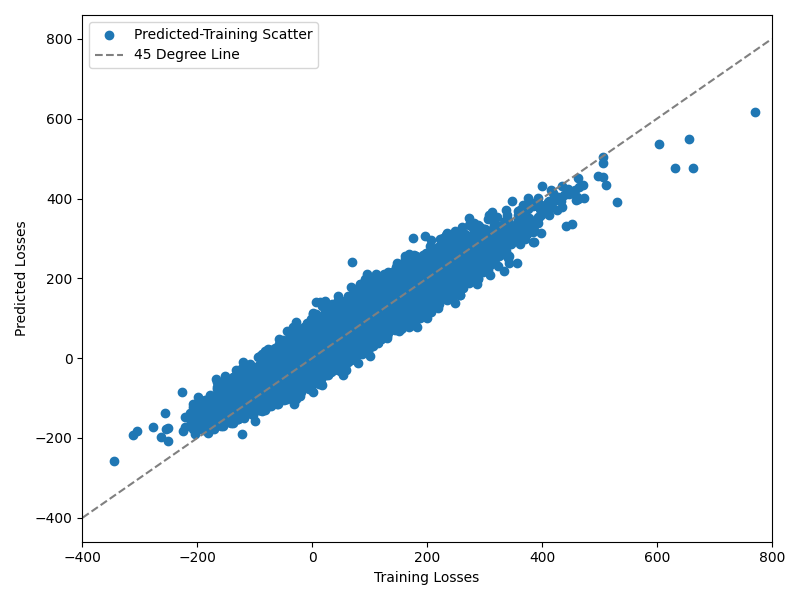
\includegraphics[width=\textwidth]{./project2/figures/2a_QQ_good_training.png}
        \caption{A good RNN metamodel}
    \end{subfigure}\hfill
    \begin{subfigure}{0.48\textwidth}
        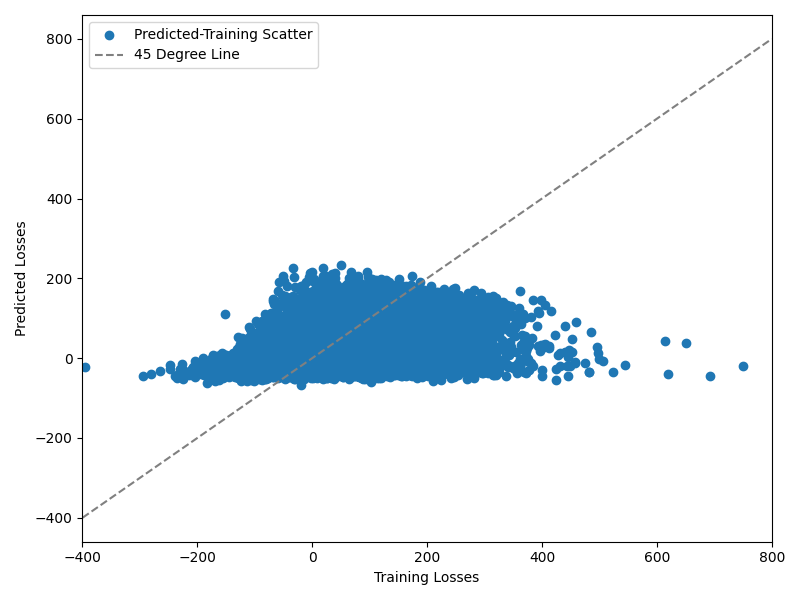
\includegraphics[width=\textwidth]{./project2/figures/2b_QQ_bad_training.png}
        \caption{A bad RNN metamodel}
        \label{subfig2:badRNN}
    \end{subfigure}
    \caption{QQ-plots between true labels (x-axis) and predicted losses (y-axis) for the RNN metamodel.} 
    \label{fig2:QQ_RNN}
\end{figure}

Recall that all three datasets are generated from the same simulation model, but the true labels contain much less simulation noise than the training and test labels.
Part of the training error is from the simulation noise, and this noise is much less reflected in the true error.
We observe that the two regression metamodels is under-fitting with high training errors. 
They also have low test and true errors, which indicates poor generalization.
In contrast, the \gls{dnn} metamodels have lower errors.
More specifically, they generalize better to the true labels than to the test labels.
The test labels contain more simulation noise than the true labels.
This is a sign of the regression metamodels' inability to learn the true feature-label relationship rather than merely over-fitting to the simulation noise in the training labels.
In practical applications, the true labels are not available.
However, analyzing the quality of fit on the true labels in a simulation environment offers a unique opportunity to understand the metamodels' true ability of learning.
Figure~\ref{fig2:QQ_REG} and Figure~\ref{fig2:QQ_NN} shows the QQ plots between the \textbf{true} loss labels and the predicted losses for the regression metamodels and the neural network metamodels, respectively.

\begin{figure}[ht!]
    \centering
    \begin{subfigure}{0.48\textwidth}
        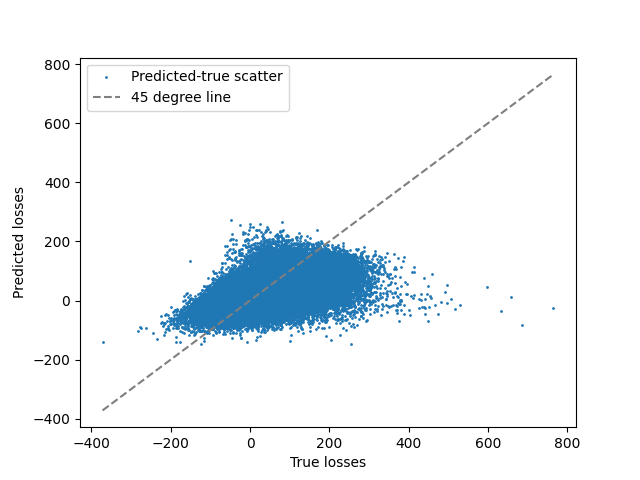
\includegraphics[width=\textwidth]{./project2/figures/qqPlots/mlrLN.png}
        \caption{MLR metamodel}
    \end{subfigure}\hfill
    \begin{subfigure}{0.48\textwidth}
        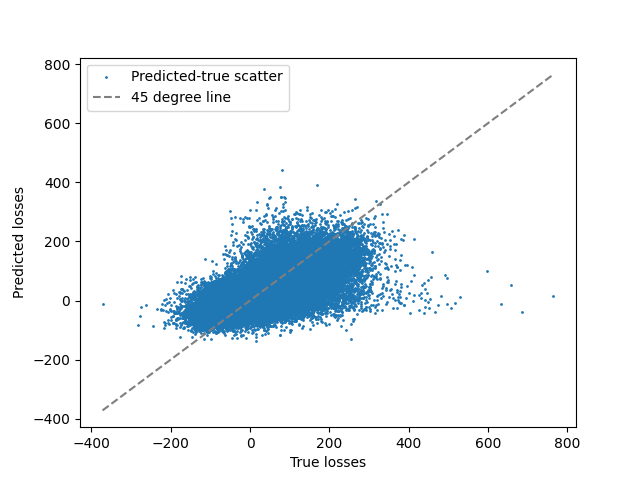
\includegraphics[width=\textwidth]{./project2/figures/qqPlots/qprLN.png}
        \caption{QPR metamodel}
    \end{subfigure}
    \caption{QQ-plots between true losses (x-axis) and predicted losses (y-axis) for regression metamodels.} 
    \label{fig2:QQ_REG}
\end{figure}

Comparing with the \gls{mse} table in Table~\ref{tab:gmwb_arch} that summarizes the overall fit, QQ plots offer a closer look at the metamodels' performance on different parts of the loss distribution.
Figure~\ref{fig2:QQ_REG} show the regression metamodel predictions and the loss labels in the true dataset.
Between the two regression metamodels, the \gls{qpr} metamodel has a slightly better fit for larger losses.
Nevertheless, the predictions of both regression metamodels are far from the true labels, and their fit on the tail is particularly undesirable.
The poor fit on the tail hinders the regression metamodels' ability to identify true tail scenarios and ultimately leads to poor \gls{cvar} estimates.
Adding the quadratic terms, our \gls{qpr} metamodel is considered as a natural extension of the \gls{mlr}.
Attempts to further improve the regression metamodels by adding interaction terms or higher-order terms do not improve the fit.
Feature engineering (i.e., variable selection) for regression metamodels is not a trivial task and is highly dependent on the simulation procedure. 
Having $240$ time-series features further complicates this issue.
As a result, our attempts to improve the traditional regression metamodels are not successful.
The regression metamodels are not flexible enough to capture the complex feature-label relationship in the dynamic hedging simulation model.

\begin{figure}[ht!]
    \centering
    \begin{subfigure}{0.48\textwidth}
        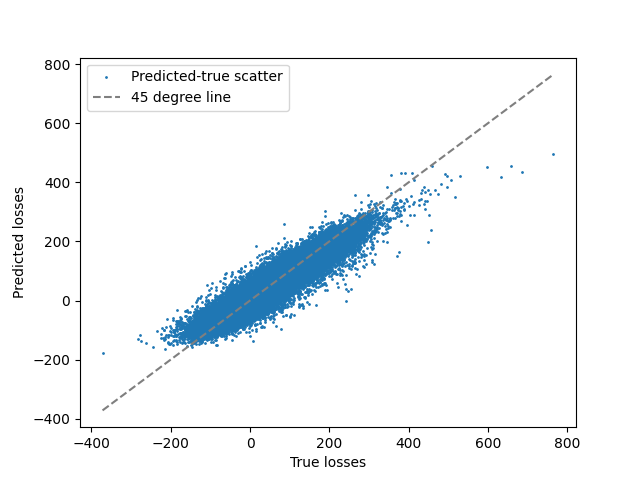
\includegraphics[width=\textwidth]{./project2/figures/qqPlots/fnnLN.png}
        \caption{FNN metamodel}
    \end{subfigure}\hfill
    \begin{subfigure}{0.48\textwidth}
        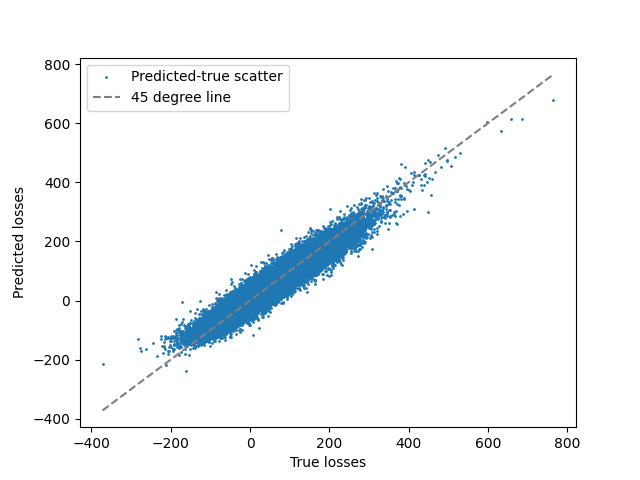
\includegraphics[width=\textwidth]{./project2/figures/qqPlots/lstmLoCapLN.png}
        \caption{LSTM metamodel}
    \end{subfigure}
    \caption{QQ-plots between true losses (x-axis) and predicted losses (y-axis) for neural network metamodels.} 
    \label{fig2:QQ_NN}
\end{figure}

In Figure~\ref{fig2:QQ_NN}, we illustrate the fit of the neural network metamodels.
The \gls{fnn} has a better fit than the regression metamodels, but it still has a poor fit on the tails.
We observe that the \gls{lstm} metamodels' QQ-plots closely follow the $45$-degree line.
Again, these metamodels are trained on noisy data, so the good fit to the true data should not be taken for granted.
This implies that these models indeed learn the true feature-label relationship in the dynamic hedging simulation model (i.e., true loss labels) even though they are trained on noisy observations (e.g., training labels) of the model.

From a unique analytical standpoint, our numerical study offers a methodical exploration into the robustness of \gls{dnn} models against noise in training labels. 
By employing the standard nested simulation procedure in Algorithm~\ref{alg2:standardProcedure} as a data generator, we gain the ability to manipulate the noise level by adjusting the number of inner replications while keeping the same simulation procedure.
This approach provides a controlled environment to examine the impact of label noise on neural network models.
It allows us to generate our true dataset that approximates the true hedging losses with a high degree of precision, and, as a result, it enables us to explore the crucial question of whether deep learning models are capable of learning the true feature-label relationship from noisy training labels.
Our numerical results in Table~\ref{tab:gmwb_arch} and the QQ plots provide direct evidence that \gls{dnn} models are indeed able to cut through the noise in the training labels and learn the true feature-label relationship.
The \gls{lstm} metamodels' ability to learn the true feature-label relationship is crucial for the two-stage procedure to identify true tail scenarios and produce accurate \gls{cvar} estimates.
Section~\ref{subsec2:noiseTolerance} discusses \gls{lstm} metamodels in more details regarding their sensitivity to data quality and quantity.
We aim at providing numerical evidence and insights into the \gls{dnn} metamodels' noise tolerance.

\subsection{Two-Stage Procedure} \label{subsec:twoStageProcedure}

We compare our two-stage procedure to a benchmark standard nested simulation procedure that runs $N=\num{1000}$ inner replications for each of the $M=\num{100000}$ outer scenarios.
In stage 1 of the proposed procedure, we first run inner simulations with $N'=100$ inner replications for each of the $M=\num{100000}$ outer scenarios.
So, stage 1's simulation budget is $10\%$ of the standard procedure's.
The resulting feature-label pairs $\{(\bS^{(i)}, \Lhat_i): i=1,\ldots,M\}$ is used for training different  metamodels.
Specifically, following the convention in machine learning literature, we split this dataset into three parts: The training, validation, and test sets have $\num{90000}$, $\num{5000}$, and $\num{5000}$ samples (representing $90\%$, $5\%$, and $5\%$ of the dataset), respectively.
At the end of stage 1, $m$ predicted tail scenarios are identified by the trained metamodels.
In stage 2, $N=\num{1000}$ inner replications are run for all predicted tail scenarios.
This is the same number of replications as the benchmark standard procedure.
Stage 2's simulation budget is $\frac{m}{M}$ of the benchmark standard procedure's.
In short, the two-stage procedure uses $15\% - 30\%$ of the benchmark procedure's budget for a safety margin between $0\% - 15\%$.
Analyzing the two stages separately, the simulation budget for stage 1 is $10\%$ of the benchmark procedure's.
Stage 2 uses $5\%$ to $20\%$ of the simulation budget of the benchmark procedure for a safety margin between $0\% - 15\%$.

In our proposed two-stage procedure, the metamodel is used to identify the predicted tail scenario set, on which the standard nested simulation procedure is run in stage 2 to estimate the $95\%$-\gls{cvar}.
An accurate identification of the true tail scenarios is crucial.
In a two-stage procedure, metamodels' overall prediction errors measured by the MSEs in Table~\ref{tab:gmwb_arch} are not the determining factor, but their ability to effectively rank the scenarios by their \textbf{true} losses is most critical in producing accurate \gls{cvar} estimates. 
A metamodel that uses less safety margin to rank can save more simulation budget in stage 2.

\begin{figure}[ht!]
    \centering
    \begin{subfigure}{0.48\textwidth}
        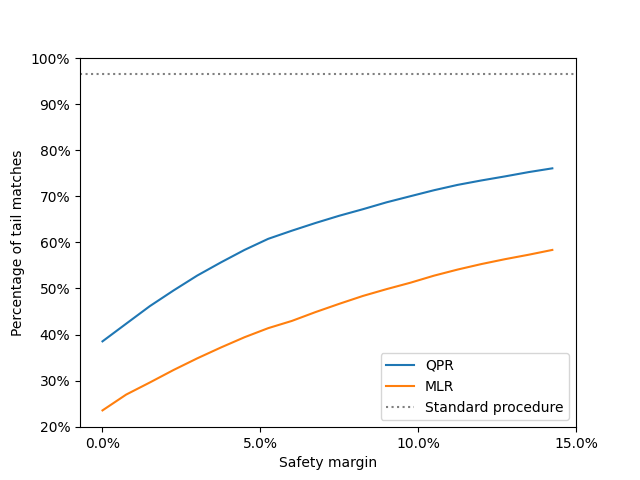
\includegraphics[width=\textwidth]{./project2/figures/tailMatches/regLN.png}
        \caption{Regression metamodels}
    \end{subfigure}\hfill
    \begin{subfigure}{0.48\textwidth}
        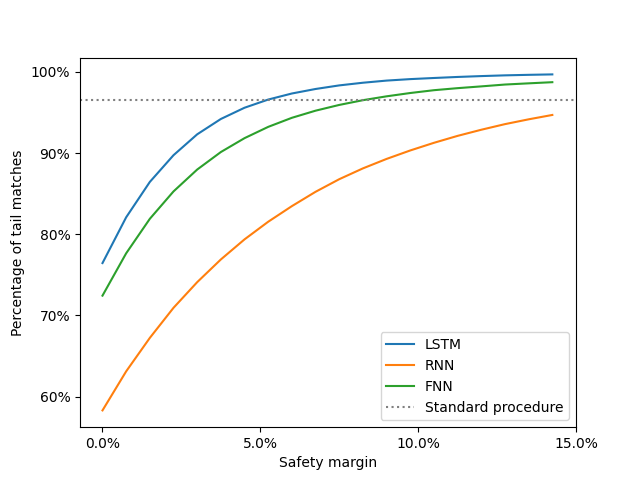
\includegraphics[width=\textwidth]{./project2/figures/tailMatches/nnLN.png}
        \caption{Neural network metamodel}
    \end{subfigure}
    \caption{Percentage of correctly identified true tail scenarios by different metamodels.}
    \label{fig2:tailMatches}
\end{figure}

Figure~\ref{fig2:tailMatches} depicts the average percentage of correctly identified true tail scenarios by different metamodels for increasing safety margins.
Each quantity is averaged over $100$ macro replications.
For a fixed safety margin, the percentage of tail matches of the traditional regression metamodels are substantially lower than the ones of the neural networks.
We observe that a poor metamodel such as the \gls{qpr} identifies less than $40\%$ of the true tail scenario without any safety margin.
In contrast, a well-suited metamodel such as the \gls{lstm} identifies more than $75\%$ of the true tail scenarios without any safety margin and more than the \gls{qpr} metamodel does with $15\%$ of safety margin\footnote{The metamodel in~\cite{dang2020efficient} identifies $100\%$ of the true tail scenarios on with a $10\%$ safety margin for a \gls{gmab} contract.
The \gls{gmab} contract is simpler than the \gls{gmwb} contract, and the true tail scenarios are easier to identify. 
For a \gls{gmab}, our \gls{lstm} metamodel identifies $100\%$ of the true tail scenarios with a $2.5\%$ safety margin}.
The \gls{rnn} metamodel suffers from the vanishing gradient problem during the training stage. 
For some macro replications (as shown in Figure~\ref{subfig2:badRNN}), the \gls{rnn} metamodels' predictions are far from the true losses, especially on the tails.
Seperating the good training macro replications from the bad ones, the results reconcile with the findings in Table~\ref{tab:gmwb_arch}.
The \gls{fnn} metamodel has a better fit than the regression metamodels, but it does not have the same level of accuracy as the \gls{lstm} metamodel, which is a specialized network to capture the sequential structure of our time-series features.
For comparison, the horizontal dotted line shows the percentage of correctly identified true tails for the standard nested simulation procedure.
A good metamodel should be able to identify a similar percentage of true tail scenarios as the standard procedure does with a reasonable safety margin.
Otherwise, the two-stage procedure will offer no computational advantage in simulation budget over the standard procedure.
The \gls{lstm} metamodel can reach similar percentage \textcolor{red}{of correctly identified true tail scenarios} with a $5\%$ safety margin.
This indicates that the \gls{lstm} metamodel should be able to reach the same level of accuracy as the standard procedure with only $20\%$ of the simulation budget.

\begin{figure}[ht!]
    \centering
    \begin{subfigure}{0.48\textwidth}
        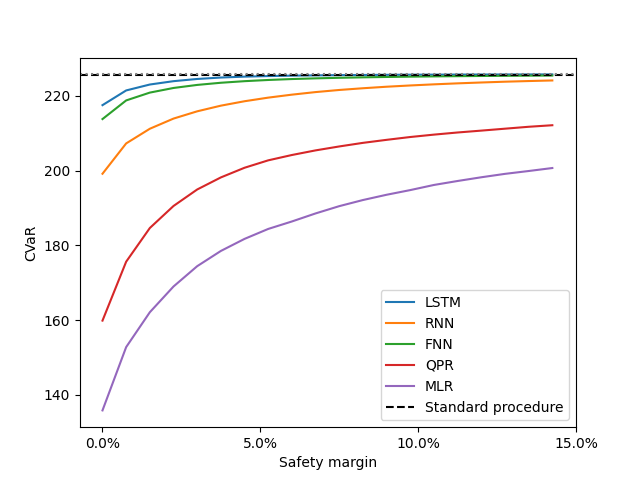
\includegraphics[width=\textwidth]{./project2/figures/CVaR/allLN.png}
        \caption{Safety margin $0\%$ - $15\%$.}
        \label{subfig2:AllSafetyMargin}
    \end{subfigure}
    \begin{subfigure}{0.48\textwidth}
        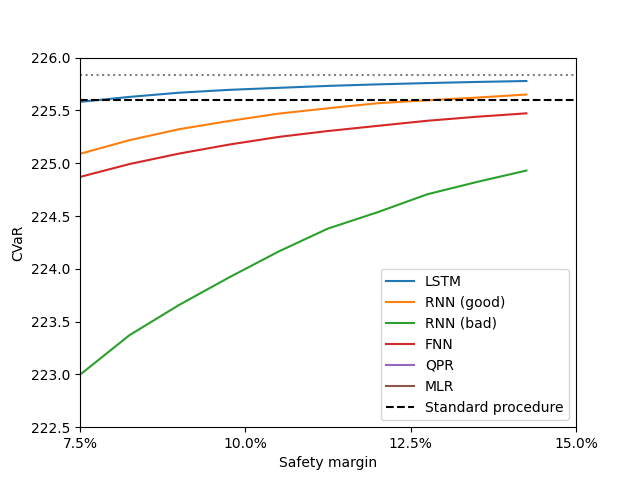
\includegraphics[width=\textwidth]{./project2/figures/CVaR/zoomedLN.png}
        \caption{Safety margin $7.5\%$ - $15\%$.}
        \label{subfig2:ZoomedSafetyMargin}
    \end{subfigure}
    \caption{Average $95\%$-CVaR estimates by different procedures. The right figure is a zoomed-in version of the left figure.} 
    \label{fig2:CVaR95}
\end{figure}

Lastly, we return to our original goal of estimating the $95\%$-\gls{cvar} of the dynamic hedging error.
Figure~\ref{fig2:CVaR95} shows the $95\%$-\gls{cvar} estimates for all five metamodels with different safety margins, averaged over $100$ macro replications.
Figure~\ref{subfig2:ZoomedSafetyMargin} is a zoomed version of Figure~\ref{subfig2:AllSafetyMargin}.
Because the safety margin only affects the two-stage procedure, the true 95\%-\gls{cvar} and the one estimated by the standard procedure are horizontal lines (which are the solid and dotted lines, respectively) in Figure~\ref{fig2:CVaR95}. 
We observe that, with reasonable safety margins, the two-stage procedures with a \gls{lstm} metamodel consistently produce estimates that are as accurate as the standard procedure's estimate.
The amount of computational savings is substantial.
The \gls{lstm} is particularly superior to other metamodels as it accurately identifies the true tail scenarios and produces highly accurate \gls{cvar} estimates with small safety margins.
By concentrating the simulation budget on the predicted tail scenarios, the two-stage procedure with the \gls{lstm} metamodel is able to achieve a similar degree of accuracy as the standard procedure with a much smaller simulation budget.
As the percentage of correctly identified tails approaches $100\%$, the two-stage procedure's \gls{cvar} estimates does not converge to the true \gls{cvar} but to the standard procedure's estimate.
This is because the two-stage procedure's \gls{cvar} estimates are based on the standard procedure's estimates on the predicted tail scenarios, and the standard procedure's estimates themselves are also noisy.

\subsection{Noise Tolerance of DNN Metamodels} \label{subsec2:noiseTolerance}

For financial and actuarial applications, regulators and practitioners are often concerned about the robustness of \gls{dnn} models to noise in training labels, which hinders the adoption of these models in practice.
Since the true relationship is unknown in real-world applications, most deep learning literature illustrates the impact of noise by artificially injecting noise into real-world datasets, which is already noisy prior to the injection.
In our numerical experiments, we are able to use Monte Carlo simulation to generate a true dataset that approximates the true hedging losses with a high degree of precision, and, as a result, we are able to explore the important question of whether deep learning models are indeed capable of learning the true feature-label relationship from noisy training labels.
In this section, we treat the standard nested simulation procedure as a data generator and examine the noise tolerance of \gls{lstm} metamodels by varying the numbers of the outer scenarios ($M$) and the inner replications ($N$) used to generate the training samples.

The number of outer scenarios corresponds to the number of feature-label pairs in the training dataset, and the number of inner replications controls the noise level in the training labels.
Recall that we use the standard nested simulation procedure with $N=100$ inner replications in our previous experiments, and we will refer to the resulting training dataset as the \textit{low-noise dataset}.
We also generate a \textit{medium-noise dataset} and a \textit{high-noise dataset} by running the standard nested simulation procedure with $N=10$ and $N=1$ inner replications, respectively.
By altering the data quantity and quality, we conduct a sensitivity analysis on the \gls{lstm} metamodels' noise tolerance.
We study the impact of noisy data on two \gls{lstm} metamodels with different model capacities, i.e., different numbers of trainable parameters.
The two \gls{lstm} metamodels has the same number of layers, but their numbers of hidden units in each layer are different.
More specfically, the high-capacity \gls{lstm} metamodel has $128$ and $16$ hidden units in the first and second \gls{lstm} layers, respectively, while the low-capacity \gls{lstm} metamodel has $32$ and $4$.

The maximum number of training samples is set to $M = \num{100000}$.
The training samples are split into training and test sets with a $90\%$-$10\%$ split ratio.
The true labels are generated by running the standard nested simulation procedure with $N=\num{100000}$ inner replications for each of the $\num{100000}$ outer scenarios.
The reason for using a maximum of $\num{100000}$ data points is precisely due to the computational cost of running the standard nested simulation procedure.
For consistency, the \gls{lstm} metamodels are trained with the same architecture and training settings as in the previous experiments.

\begin{table}[ht!]
    \small
    \centering
    \begin{tabular}{lccccc}
        \toprule
        \textbf{Model}      & \textbf{$N$}         & \textbf{Training error}                & \textbf{Test error}               & \textbf{True error}\\
        \midrule
        \gls{lstm}                & $\num{100}$                & $0.075 (\pm4.5\times 10^{-3})$         & $0.079(\pm5.4\times 10^{-3})$     & $0.063 (\pm4.4\times 10^{-3})$ \\ 
        High-capacity \gls{lstm}  & $\num{100}$                & $0.068 (\pm3.6\times 10^{-3})$         & $0.102(\pm6.1\times 10^{-2})$     & $0.060 (\pm3.6\times 10^{-3})$ \\
        Average Difference  & $\num{100}$                & $-0.007$                               & $0.023$                           & $-0.003$ \\
        \hline
        \gls{lstm}                & $\num{10}$                 & $0.195 (\pm1.1\times 10^{-3})$         & $0.193(\pm1.7\times 10^{-3})$     & $0.070 (\pm9.1\times 10^{-4})$ \\
        High-capacity \gls{lstm}  & $\num{10}$                 & $0.157 (\pm2.0\times 10^{-3})$         & $0.199(\pm1.9\times 10^{-3})$     & $0.065 (\pm1.9\times 10^{-3})$ \\
        Average Difference  & $\num{10}$                 & $-0.038$                               & $0.006$                           & $-0.005$ \\
        \hline
        \gls{lstm}                & $\num{1}$                  & $1.366 (\pm8.6\times 10^{-3})$         & $0.781(\pm6.0\times 10^{-3})$     & $0.129 (\pm5.0\times 10^{-3})$ \\
        High-capacity \gls{lstm}  & $\num{1}$                  & $1.354 (\pm2.7\times 10^{-2})$         & $0.795(\pm8.3\times10^{-2})$      & $0.149 (\pm2.7\times 10^{-2})$ \\
        Average Difference  & $\num{1}$                  & $-0.012$                               & $0.014$                           & \textcolor{red}{$0.020$} \\
        \bottomrule
    \end{tabular}
    \caption{MSEs of LSTM metamodels.}
    \label{tab:lstm_arch}
\end{table}

The first two rows of Table~\ref{tab:lstm_arch} shows the average squared errors and the half widths of their $95\%$ confidence intervals between the metamodel predictions and the labels in the training dataset and the true dataset.
$N$ indicates the noise level in the training labels, i.e., a simulation dataset with fewer inner replications has a higher noise level.
The test errors are included as a practical measure of the metamodels' generalization ability to unseen noisy samples.
For this particular experiment, we are more interested in the true errors, which measure the metamodels' ability to learn the true feature-label relationship from the low-noise, medium-noise, and high-noise datasets.
We first observe that all the true errors are lower than the training errors, indicating that the \gls{lstm} metamodels generalize well to predicting the true losses.
Both \gls{lstm} metamodels are able to learn the true feature-label relationship from the low-noise and medium-noise datasets.
However, when the noise level is high, both \gls{lstm} metamodels have high true errors.

The differences in the errors between the \gls{lstm} metamodels are also reported in the last rows of Table~\ref{tab:lstm_arch}.
A positive difference indicates that the high-capacity \gls{lstm} has a higher error than the regular \gls{lstm}.
We observe that both \gls{lstm} metamodels have similar errors on the low-noise and medium-noise datasets.
However, when the noise level is high, the high-capacity \gls{lstm} has higher errors than the regular \gls{lstm}.
This is because the high-capacity \gls{lstm} has more trainable parameters and is more prone to over-fitting to the noise in the training labels.
In contrast, the \gls{lstm} metamodel is more robust to label noise and is able to learn the true feature-label relationship better from the high-noise dataset.
In practice, since the true relationship is unknown, the true error is not readily available.
The test error approximates the true error and is directly observable.
The differences in test errors of the \gls{lstm} metamodels are inconsistent with the differences in true errors.
Therefore, test errors are not reliable indicators of the metamodels' noise tolerance.
For practical applications that utilize nerual networks as metamodels, we recommend not to simulate the test scenarios.
Instead, we recommend simulating the true contract losses on a subset of training scenarios to evaluate the metamodels' generalization ability.

In summary, our numerical experiments demonstrate that both \gls{lstm} metamodels are capable of learning the true inner simulation model from the noisy training labels.
In most cases, a high-capacity metamodel is shown to perform better.
Nevertheless, in extreme circumstances when the noise level is too high, using a high capacity metamodel leads to severe over-fitting and poor generalization.
Hence, domain knowledge about the right architecture for the task and knowledge about the noise level in the training labels are beneficial for choosing the correct metamodel.

\begin{figure}[ht!]
    \centering
    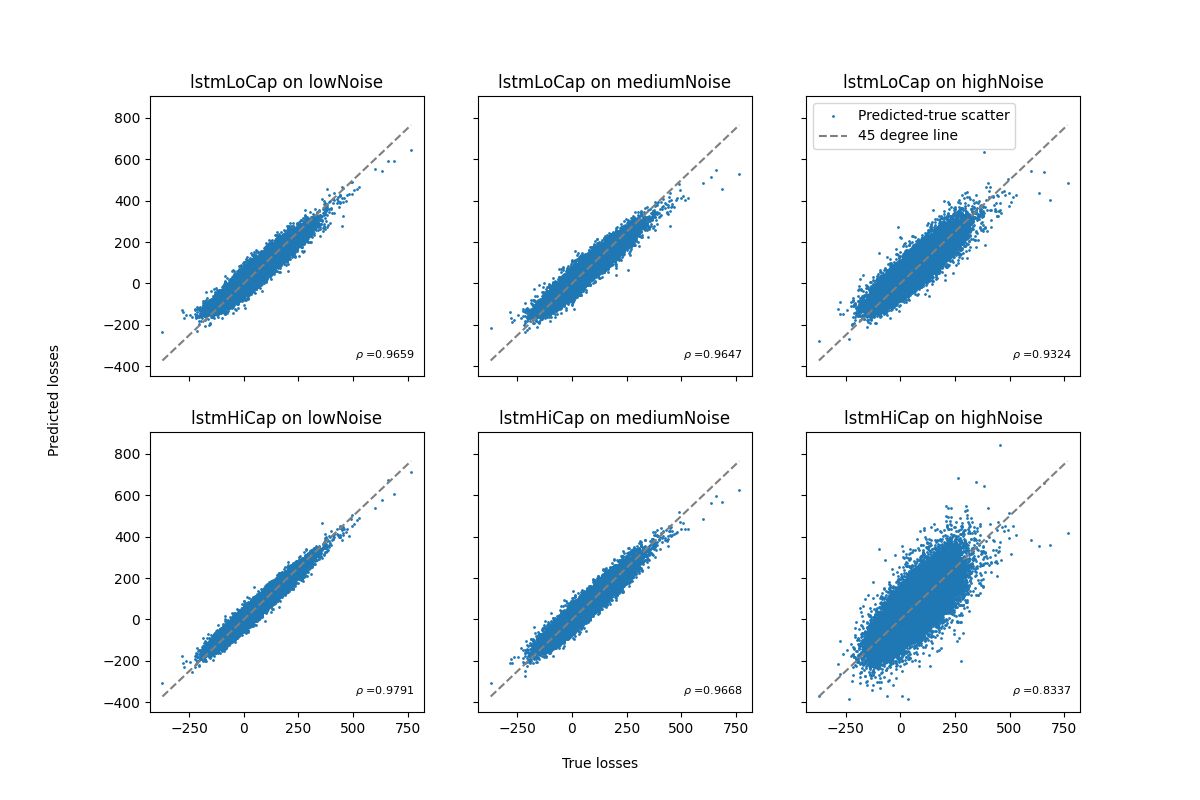
\includegraphics[width=\textwidth]{./project2/figures/qqPlots/lstmAll.png}
    \caption{QQ-plots between true losses (x-axis) and predicted losses (y-axis) for two LSTM metamodels.} 
    \label{fig2:QQ_All}
\end{figure}

In further details, the QQ-plots depicted in Figure~\ref{fig2:QQ_All} illustrates the fit of the two \gls{lstm} metamodels when different noise levels are present in the training labels.
They are arranged in a 2-by-3 grid, where the two rows correspond to the two \gls{lstm} metamodels with different model capacities, and the three columns correspond to the increasing noise levels.
The Pearson correlation coefficient between the true losses and the predicted losses is labeled in each subplot.
The sparsity of the plot increases as we move from left to right, indicating that the noise level in the training labels increases.
There are two key findings.
\begin{enumerate}
    \item   When trained on the low-noise dataset, the metamodel predictions of high-capacity \gls{lstm} align more closely with the true labels than the regular \gls{lstm}.
    This is expected because the high-capacity \gls{lstm} has more trainable parameters and is able to learn more complex relationships better when the noise level is low.
    \item   When the noise level is medium or high, the high-capacity \gls{lstm} is more affected than the regular \gls{lstm}.
    This is because the high-capacity \gls{lstm} has more trainable parameters and is more prone to over-fitting to the noise in the training labels.
    In contrast, the regular \gls{lstm} is more robust to label noise.
\end{enumerate}

To further test the sensitivity of a \gls{lstm} metamodel and provide a more comprehensive view of the noise tolerance of \gls{dnn} models, we conduct a sensitivity analysis on the noise tolerance of the regular \gls{lstm} metamodel by varying the numbers of outer scenarios ($M$) and inner replications ($N$) used to generate the training dataset.
The number of outer scenarios corresponds to the number of data points in the training dataset, and the number of inner replications controls the noise level in the training labels.

\begin{table}[ht!]
    \small
    \centering
    \begin{tabular}{lccccc}
        \toprule
                            & $N=\num{1}$ & $N=\num{10}$  & $N=\num{100}$ & $N=\num{1000}$\\
        \midrule
        $M = \num{100}$      & $1.139$ & $0.229$ & $0.167$ & $0.158$ \\
        $M = \num{1000}$     & $0.559$ & $0.173$ & $0.123$ & $0.127$ \\
        $M = \num{10000}$    & $0.283$ & $0.115$ & $0.099$ & $0.097$ \\
        $M = \num{100000}$   & $0.129$ & $0.070$ & $0.063$ & $0.063$ \\
        \bottomrule
    \end{tabular}
    \caption{MSE between regular LSTM predicted losses and true losses.}
    \label{tab2:lstm_sens}
\end{table}

\begin{table}[ht!]
    \small
    \centering
    \begin{tabular}{lccccc}
        \toprule
                          & $N=\num{1}$ & $N=\num{10}$  & $N=\num{100}$ & $N=\num{1000}$\\
        \midrule
        $M = \num{100}$      & $0.764$ & $0.408$ & $0.131$ & $0.087$ \\
        $M = \num{1000}$     & $0.878$ & $0.367$ & $0.156$ & $0.087$ \\
        $M = \num{10000}$    & $0.351$ & $0.147$ & $0.064$ & $0.063$ \\
        $M = \num{100000}$   & $0.149$ & $0.065$ & $0.060$ & $0.038$ \\
        \bottomrule
    \end{tabular}
    \caption{MSE between high-capacity LSTM predicted losses and true losses.}
    \label{tab2:hicaplstm_sens}
\end{table}

Table~\ref{tab2:lstm_sens} and~\ref{tab2:hicaplstm_sens} show the average squared errors between the \gls{lstm} predictions and the true losses for increasing $M$ and $N$.
The last rows of Table~\ref{tab2:lstm_sens} and Table~\ref{tab2:hicaplstm_sens} show the performance of the regular and high capacity \gls{lstm} metamodels trained with $M=\num{100000}$ training labels with different noise levels.
We observe that an increasing $N$ reduces the \gls{mse}, but the reduction is not substantial for a regular \gls{lstm} when $N$ is larger than $\num{10}$.
For the high-capacity \gls{lstm}, the \gls{mse} is substantially reduced when $N$ is increased from $\num{1}$ to $\num{100}$, but the reduction is not substantial when $N$ is increased from $\num{100}$ to $\num{1000}$.
Another way to interpret the results in Table~\ref{tab2:lstm_sens} is to compare the MSEs for the same budget of $\Gamma = M \times N$. 

Table entries on the same off-diagonal have the same simulation budget $\Gamma$.
For most budgets, the MSEs are also the lowest when $N = 10$.
The results in Table~\ref{tab2:lstm_sens} suggest that the performance of the \gls{lstm} metamodel is more sensitive to the number of outer scenarios than the number of inner replications.
Treating the neural network as an advanced regression metamodel, we find this pheonomenon to be consistent with the results in~\cite{broadie2015risk}, where the authors show that the performance of a regression-based nested simulation procedure is more affected by the number of outer scenarios.
The last row in Table~\ref{tab2:lstm_sens} and ~\ref{tab2:hicaplstm_sens} show that the high-capacity \gls{lstm} metamodel is relatively insensitive to the number of inner replications.
To make the most efficient use of a fixed simulation budget, the number of inner replication should be set constant around $N=10$ while increasing the number of outer scenarios to the maximum.

To further investigate the \gls{lstm} metamodels' sensitivity to data quantity and quality ($M$ and $N$, respectively), we report the Spearman rank correlation coefficients Table~\ref{tab2:lstm_corr}, which measure the ability to rank the scenarios by their true losses.
It is an appropriate measure of the metamodel's performance in the two-stage procedure, where the metamodel is used to identify the predicted tail scenario set, on which extensive simulations are run in stage 2 to estimate the $95\%$-\gls{cvar}.
The Pearson correlation coefficients are also included in the parentheses to illustrate the linear correlation between the predicted losses and the true losses.
They measure the metamodel's overall prediction accuracy.
Our previous numerical experiments illustrated in Figure~\ref{fig2:tailMatches} have shown that the \gls{lstm} metamodel predictions have high \textit{Spearman} correlation with the true labels for the combination $M=\num{100000}$ and $N=\num{100}$.
We intend to examine if \gls{lstm} predictions also have high \textit{Pearson} correlation with the true labels.
A high \textit{Pearson} correlation suggests the possibility of using \gls{lstm} predictions to estimate risk measures directly.

\begin{table}[ht!]
    \small
    \centering
    \begin{tabular}{lccccc}
        \toprule
                           & $N=\num{1}$   & $N=\num{10}$  & $N=\num{100}$ & $N=\num{1000}$ \\
        \midrule
        $M = \num{100}$    & 0.638 (0.881) & 0.875 (0.915) & 0.896 (0.903) & 0.937 (0.941) \\
        $M = \num{1000}$   & 0.722 (0.768) & 0.899 (0.908) & 0.886 (0.891) & 0.922 (0.927) \\
        $M = \num{10000}$  & 0.845 (0.630) & 0.937 (0.900) & 0.908 (0.905) & 0.947 (0.948) \\
        $M = \num{100000}$ & 0.935 (0.640) & 0.963 (0.909) & 0.927 (0.922) & 0.965 (0.966) \\
        \bottomrule
    \end{tabular}
    \caption{Spearman (Pearson) correlation coefficients of high-capacity LSTM predictions.}
    \label{tab2:lstm_corr}
\end{table}

Consistent with our previous numerical experiments, the Spearman correlations of a high-capacity \gls{lstm} is high for a moderate simulation budget. 
For $M= \num{100000}$, the Spearman correlation is relativelyinsensitive to $N$.
This finding supports further budget savings for our two-stage procedure.
In stage 1, we can lower $N$ from $\num{100}$ to $\num{10}$ almost without compromising on tail scenario preditions. 

For an entry of Table~\ref{tab2:lstm_corr}, the total simulation budget $\Gamma = M N$. 
Entries on the same off-diagonal all have the same $\Gamma$.
The Pearson correlation coefficients are substantially lower for $N=\num{1}$ than the other $N$ values.

\begin{figure}
    \centering
    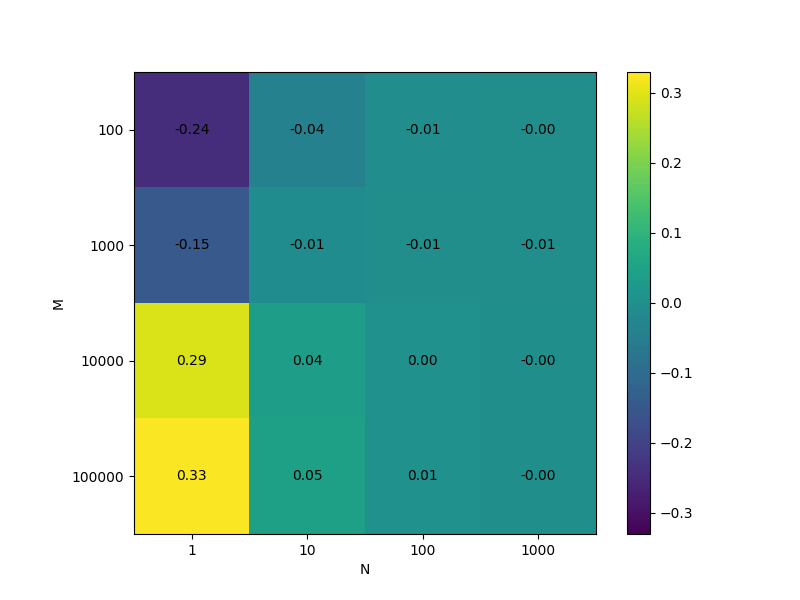
\includegraphics[width=0.6\textwidth]{./project2/figures/cor_heatmap.png}
    \caption{Difference between Spearman and Pearson correlations for high-capacity LSTM metamodel.}
    \label{fig2:cor-heatmap}
\end{figure}

Figure~\ref{fig2:cor-heatmap} shows the difference between the Spearman and Pearson correlation coefficients for the high-capacity \gls{lstm} metamodel.
The heatmap is generated by subtracting the Pearson correlation coefficients from the Spearman correlation.
We observe that Spearman correlation coefficients are not substantially different from the Pearson correlation coefficients for any $N$ larger than $\num{10}$. 
This is a strong evidence that the \gls{lstm} metamodel is not only able to effectively rank the scenarios by their true losses, but also able to make accurate loss predictions.
Instead of using the \gls{lstm} metamodel only for classifying tail scenarios in a two-stage procedure, \gls{lstm}'s ability to cut through a moderate level of noise in training labels encourages us to use its predictions to estimate the \gls{cvar} directly. 

\subsection{Single-Stage Procedure}

The accuracy and robustness of the \gls{lstm} metamodels motivate us to propose a single-stage procedure that uses the metamodel predictions to estimate the \gls{cvar} directly. 
Instead of relying on the standard nested simulation procedure in stage 2, the single-stage procedure can be even more efficient.
In this section, we compare the single-stage procedure to the two-stage procedure and the standard procedure in estimating the $95\%$-\gls{cvar} of the hedging losses for \gls{gmwb}.
In our numerical experiments, the results for the single-stage procedure is obtained with the same metamodels as in the two-stage procedure.
The only difference from Section~\ref{subsec:twoStageProcedure} is that the metamodel predictions are used to estimate the risk measures directly.

\begin{figure}[ht!]
    \centering
    \begin{subfigure}{0.48\textwidth}
        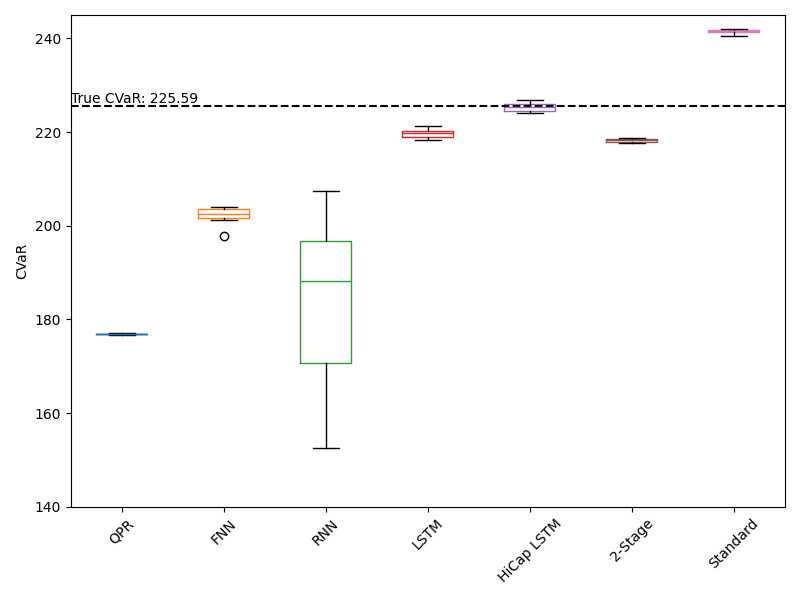
\includegraphics[width=\textwidth]{./project2/figures/singleStage/CVaRmediumNoise.png}
        \caption{Medium noise training labels ($N=10$)}
    \end{subfigure}
    \begin{subfigure}{0.48\textwidth}
        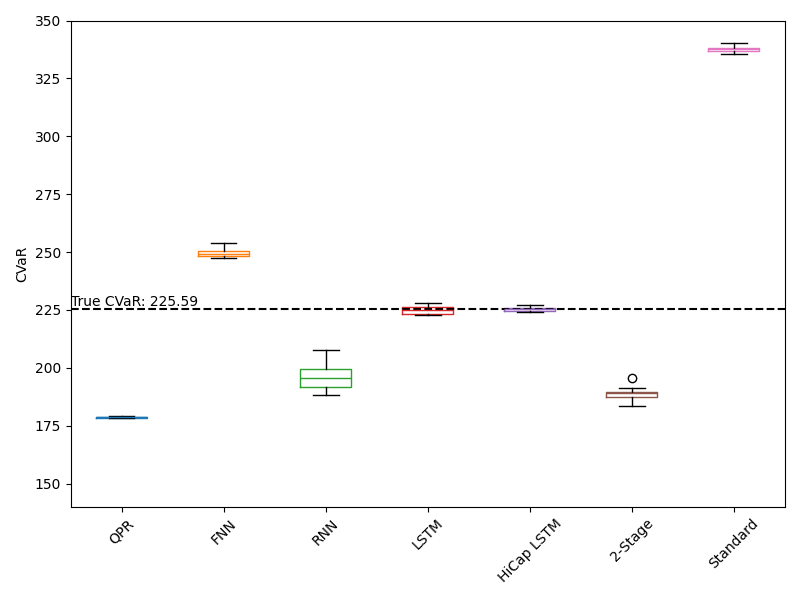
\includegraphics[width=\textwidth]{./project2/figures/singleStage/CVaRhighNoise.png}
        \caption{High noise training labels ($N=1$)}
    \end{subfigure}
    \caption{CVaR estimates of the single-stage procedure with metamodels.}
    \label{fig2:CVaRsingleStage}
\end{figure}

Figure~\ref{fig2:CVaRsingleStage} shows the boxplots of the 95\%-\gls{cvar} estimates of the single-stage procedure with different metamodels and compares them to the two-stage procedure and the standard procedure.
The two-stage procedure uses the same simulation budget as the single-stage procedure in stage 1 with an extra amount of budget for an  extensive inner simulation on the predicted tail scenarios in stage 2.
The metamodel with the best performance in the two-stage procedure is selected, and the safety margin is set to $0\%$.
The standard procedure shown in Figure~\ref{fig2:CVaRsingleStage} uses the noisy loss labels in the training dataset to estimate the \gls{cvar} directly, which uses the same simulation budget as the single-stage procedure.
We observe that the single-stage procedures with the regular \gls{lstm} metamodel consistently produce \gls{cvar} estimates that are closer to the true value than the standard procedure's estimate.
This finding is especially impressive when the noise level in the training labels is high.
It is another strong evidence that a well-selected \gls{lstm} metamodel is able to cut through the noise in the noisy training labels and make accurate loss predictions that lead to accurate \gls{cvar} estimates.
The difference in performance among the metamodels is more pronounced in the single-stage procedure than in the two-stage procedure.
Trained using medium noise labels, the high-capacity \gls{lstm} metamodel consistently produces \gls{cvar} estimates that are closer to the true value than the regular \gls{lstm}, while the other metamodels produce worse estimates.

However, when the noise level in the training labels is high, the high-capacity \gls{lstm} suffers from severe overfitting. 
This is also evident in Table~\ref{tab:lstm_arch}.
Since we are using the metamodel predictions to estimate the \gls{cvar} directly without any safety margin, the metamodel's overall prediction accuracy becomes more important.
In other words, the single-stage procedure is more sensitive to the metamodel's ability to make accurate loss predictions than the two-stage procedure.
Previously, a generic \gls{fnn} metamodel performs well in the two-stage procedure. 
However, results in Figure~\ref{fig2:CVaRsingleStage} suggest that the \gls{fnn} metamodel should not be used in the single-stage procedure.

A single-stage procedure with a regular \gls{lstm} metamodel is particularly superior to the two-stage procedure, as it is able to achieve a higher accuracy as the standard procedure with a much smaller amount of simulation budget.
Note that the single-stage procedure does not require a safety margin.
By avoiding the calibration of the safety margin, it is more straight-forward to implement and is more efficient than the two-stage procedure.
For a two-stage procedure with a $0\%$ safety margin, the extra computational cost is from the extensive inner simulation in stage 2.
On $4$ $20$-core Intel Xeon Gold $\num{6230}$ processors, stage 2 of the two-stage procedure takes $30$ minutes to run with parallel processing, while the $95\%$ confidence band of training time of the high-capacity \gls{lstm} metamodel is $(19.64 \pm 0.94)$ minutes on an Nvidia RTX $\num{3060}$ Ti GPU.
While the accuracy of the two-stage procedure is highly dependent on the safety margin, increasing the safety margin introduces extra computational cost.
Therefore, while achieving a higher accuracy in estimating the \gls{cvar}, the single-stage procedure requires only $60\%$ computation time of the two-stage procedure.

\begin{figure}[ht!]
    \centering
    \begin{subfigure}{0.48\textwidth}
        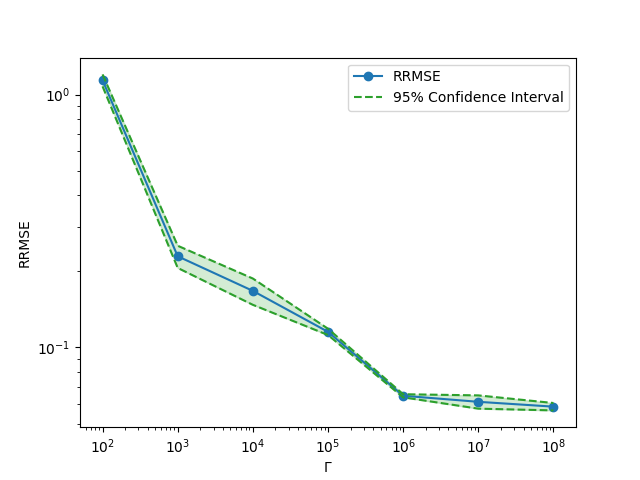
\includegraphics[width=\textwidth]{./project2/figures/singleStage/MSEConvergence_lstmLoCap.png}
        \caption{Regular LSTM}
        \label{subfig2:convLoCap}
    \end{subfigure}
    \begin{subfigure}{0.48\textwidth}
        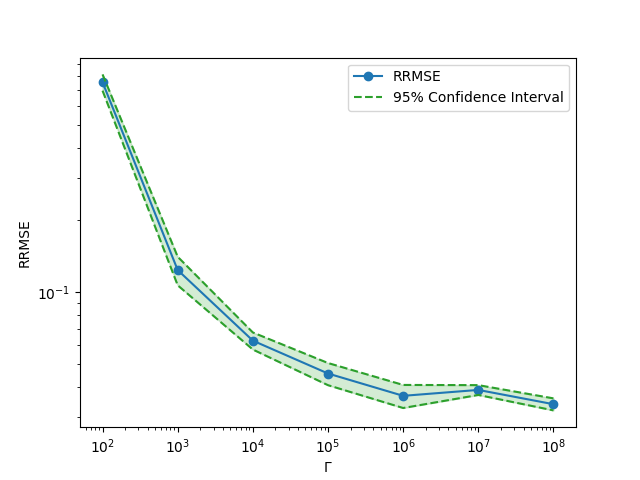
\includegraphics[width=\textwidth]{./project2/figures/singleStage/MSEConvergence_lstmHiCap.png}
        \caption{High-capacity LSTM}
        \label{subfig2:convHiCap}
    \end{subfigure}
    \caption{Empirical convergence of CVaR for the single-stage procedure with LSTM metamodels.} 
    \label{fig2:gammaConvergence}
\end{figure}


To further investigate the single-stage procedure's performance, we conduct a convergence analysis on the \gls{lstm} metamodels.
Figure~\ref{fig2:gammaConvergence} shows the log-log plots of the \gls{rrmse} between the \gls{lstm} metamodel \gls{cvar} predictions and the true \gls{cvar} against the total simulation budget $\Gamma$.
For each budget $\Gamma$, the metamodels are trained for different combinations of $M$ and $N$, and the metamodel with the best \gls{rrmse} is plotted.
While numerical results suggest that the \gls{cvar} estimator of the single-stage procedure with \gls{lstm} metamodels may have better accuracy than the two-stage procedure and the standard procedure when the number of outer scenarios is further increased, we found it difficult to compare their performance due to insufficient computational resources.
For $\Gamma \leq \num{100000}$, the number of outer scenarios is fixed at $M = \num{100000}$, and only the number of inner replications is varied.
Instead, we try to analyze the effect of the number of outer scenarios and the number of inner replications separately by fixing one and varying the other.

\begin{figure}[ht!]
    \centering
    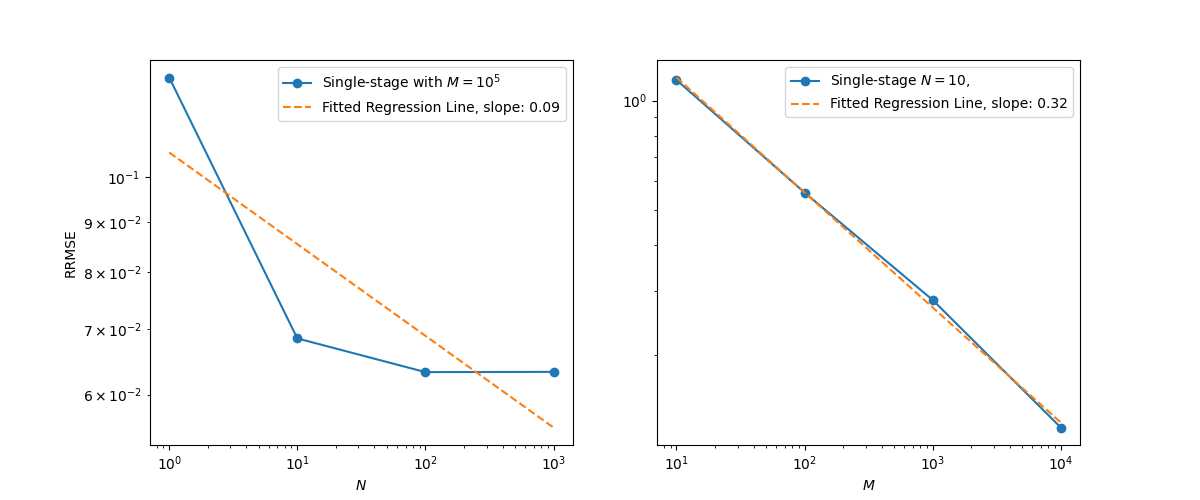
\includegraphics[width=\textwidth]{./project2/figures/singleStage/MSEConvergence_lstmLoCap_MN.png}
    \caption{Empirical convergence of the single-stage procedure with a LSTM metamodel.} 
    \label{fig2:mnConvergence}
\end{figure}

Figure~\ref{fig2:mnConvergence} shows the log-log plots of the \gls{rrmse} between the \gls{lstm} metamodel \gls{cvar} predictions and the true \gls{cvar} against the simulation budget.
The left figure shows the empirical convergence of the \gls{rrmse} for increasing inner replications with a fixed number of outer scenarios ($M=\num{100000}$), and the right figure shows the empirical convergence of the \gls{rrmse} for increasing outer scenarios with a fixed number of inner replications ($N=\num{10}$).
Due to computational constraints, we are not able to run the two-stage procedure and the standard procedure with more outer scenarios or more inner replications, therefore the comparison between the single-stage procedure is only available up to $M = \num{100000}$ and $N = \num{1000}$.
We observe that the \gls{rrmse} decreases as the simulation budget increases, and the rate of convergence is higher when the quantity of the data increases.
For an \gls{lstm} metamodel, increasing the data quality of the training labels has diminishing returns, which is consistent with the results in Figure~\ref{fig2:mnConvergence}.
For an increasing number of inner replications with a fixed number of outer scenarios, the \gls{rrmse} ceases to decrease after reaching $N = \num{100}$. 
More specfically, when the quality of the training labels is fixed at $N = \num{10}$, the \gls{cvar} estimator of a single-stage procedure with a \gls{lstm} metamodel converge roughly in the order of $\mathcal{O}(M^{\frac{2}{3}})$.
This observation resonates with the best possible convergence rate of a standard nested simulation procedure in~\cite{gordy2010nested}.
Hence, in practice, we suggest running the single-stage procedure with a moderate number of inner replications and a large number of outer scenarios to achieve a high level of accuracy with a reasonable computational cost.


\section{Conclusion} \label{sec2:conclusion}
The proposed nested simulation procedures with \gls{dnn} metamodels are shown to result in substantial computational savings in estimating \gls{cvar} of the hedging loss of a \gls{va} contract from accurately predicting the hedging losses and identifying the tail scenarios.
When new outer scenarios are generated, a trained \gls{lstm} metamodel can distinguish between tail and non-tail scenarios and make accurate predictions without the need to run new inner simulations.

Our novel experiment design allows us to examine the impact of label noise on \gls{dnn} models.
We find that a \gls{dnn} with a suitable architecture is able to cut through the noise in training labels and learn the true complex dynamic hedging model.
By showcasing the resilience of these models, our study aims at encouraging regulatory bodies to recognize the value and applicability of deep learning metamodels in financial risk management, and it provides informed suggestions and guidance for the incorporation and oversight of advanced deep learning metamodel in Monte Carlo Simulation in financial applications.
Our findings are particularly insightful in this context.

In our numerical experiments, a \gls{lstm} metamodel is resilient to a high level of noise in training labels and is able to make accurate predictions. 
This is an encouraging evidence that \gls{dnn} metamodels can be used to improve the efficiency of Monte Carlo simulation for quantitative risk management tasks that require a computational-expensive simulation procedure.
We propose two nested simulation procedures that use \gls{dnn} metamodels to estimate risk measures of the hedging loss of a \gls{va} contract.
For estimating tail risk measures, our two-stage procedure is designed to address regulatory concerns by avoiding the direct use of metamodel predictions but instead by using them to identify the potential tail scenarios.
An extensive inner simulation is performed in this chapter to achieve a high level of accuracy on the predicted tail scenarios.
However, the safety margin in the two-stage procedure is a user's choice and is not easy to determine before running extensive numerical experiments.

Our single-stage procedure uses the metamodel predictions to estimate the risk measure directly.
It is more efficient and can be extended to estimate risk measures that require knowledge of the entire loss distribution.
Our numerical experiments demonstrate that the proposed single-stage procedure with \gls{dnn} metamodels result in further computational savings over our two-stage procedure. 
Furthermore, our numerical results provide evidences for adopting \gls{dnn} metamodels in Monte Carlo simulation for risk management tasks.
Through our systematic empirical study of the noise tolerance of \gls{dnn} metamodels, we address regulatory concerns by showing that a \gls{lstm} metamodel with moderate model capacity is resilient to a high level of noise in training labels and is able to make accurate predictions.
A possible future research direction is to apply \gls{dnn} metamodels in other financial risk management tasks that requires complex nested simulation with high-dimensional outer scenarios.
Another future research direction is to investigate the impact of label noise on other deep learning models, such as convolutional neural networks and transformer models, and to compare their performance with \gls{lstm} metamodels in nested simulation procedures. 
From a practical standpoint, the choice of a suitable \gls{dnn} architecture is crucial for the success of a deep learning metamodel in nested simulation procedures.
We find that a \gls{lstm} metamodel is the most suitable for our dynamic hedging simulation model with time series features, but the optimal network architecture may vary for different simulation models.
Exploring \gls{dnn} metamodels in other complex risk management tasks presents a promising avenue for research, especially as these tasks often involve complex, high-dimensional scenarios where traditional methods are insufficient. 
The versatility of neural networks could unlock new insights across a broad spectrum of financial and actuarial applications.

In this chapter, we have demonstrated the potential of \gls{dnn} metamodels to estimate risk measures with high accuracy and efficiency when simulation data is abundant.
In practice, simulation data is often scarce for new market conditions and new insurance products.
\gls{dnn} metamodels are known to suffer from over-fitting when the number of training samples is limited.
In the next chapter, we will extend our study to transfer learning and show that \gls{dnn} metamodels trained on an existing \gls{va} contract can be transferred to a new \gls{va} contract with different market conditions.
We hypothesize that the \gls{dnn} metamodel will generalize well to the new \gls{va} contract, and the computational savings from transfer learning will be substantial.
\chapter{Transfer Learning for Rapid Adaptation of Deep Neural Network Metamodels in Dynamic Hedging of Variable Annuities} \label{chap:project3}

\section{Introduction}

In the evolving landscape of financial markets, insurance products such as VAs have gained significant interest due to their ability to provide both investment growth and guaranteed benefits. 
Managing the risks associated with these products, especially in volatile market conditions, is a complex task that demands sophisticated financial modeling techniques. 
Traditional machine learning models often struggle to capture the intricate nonlinear relationships and temporal dependencies inherent in financial data.
To address the computational burden, metamodeling techniques have been proposed, where a simpler model approximates the outcomes of the more complex simulation. 
In particular, deep neural networks (DNNs), and specifically LSTM networks, have been employed as metamodels to predict the outcomes of the inner simulations efficiently
Chapter~\ref{chap:project2} introduces a nested simulation framework for dynamic hedging of VAs, where the inner simulation is approximated by an LSTM metamodel.
It shows that crude RNN and LSTMs are well-suited for metamodeling Monte Carlo simulation of financial time series and can capture the long-term dependencies in the data.

Despite the advantages of using DNN metamodels, a significant challenge arises when market conditions change or new VA contracts with different features are introduced. 
Retraining neural network metamodels from scratch in response to every change is computationally inefficient and time-consuming.
Moreover, financial markets are inherently dynamic, with frequent shifts in volatility, interest rates, and other risk factors~\citep{cont2001empirical}.
Therefore, it is essential to develop methods that can rapidly adapt existing metamodels to new conditions without incurring the full computational cost of retraining.
Transfer Learning offers a compelling solution to this problem by enabling the reuse of a pre-trained model on a new but related task~\citep{pan2009survey}.
In the context of DNNs, transfer learning involves leveraging the knowledge acquired during training on one dataset to improve learning performance on a different dataset~\citep{yosinski2014transferable}.
This approach can significantly reduce training time and computational resources while enhancing model generalization.
Instead of starting from scratch, a new DNN metamodel can be built on top of the pre-trained model and fine-tuned on the new data, allowing it to adapt quickly to changing market conditions and new VA contracts.

In this chapter, we explore the application of transfer learning to the dynamic hedging of VAs using RNN and LSTM metamodels.
We propose a novel transfer learning framework that accelerates the training of DNN metamodels for nested simulatiogn in a dynamic hedging problem.
Our approach involves pre-training an LSTM network on a large dataset of VA simulations and then fine-tuning it on a smaller dataset of new VA contracts.
We evaluate the performance of the transfer learning framework on a real-world dataset of VA contracts and compare it with training the LSTM network from scratch.

The rest of this chapter is organized as follows.
Section~\ref{sec3:background} provides an overview of the dynamic hedging problem for VAs and the use of LSTM networks as metamodels in a nested simulation procedure.
Section~\ref{sec3:transfer_learning} introduces the transfer learning framework for rapid adaptation of LSTM metamodels in dynamic hedging.
Section~\ref{sec3:experiments} presents the experimental setup and results, comparing the performance of transfer learning with training from scratch.
Finally, Section~\ref{sec3:conclusion} concludes the chapter and discusses future research directions.

\section{Transfer Learning in Financial Metamodeling} \label{sec3:background}

Transfer learning (TL) is a machine learning paradigm where knowledge acquired from a source task is utilized to improve learning performance on a related target task.
One of the primary applications of TL in finance is asset price prediction. 
Traditional models, such as autoregressive integrated moving average (ARIMA) and generalized autoregressive conditional heteroskedasticity (GARCH), have been widely used in time series modeling.
However, these models often struggle to capture the complex patterns and nonlinear relationships in financial data.
DNNs like RNN and LSTM networks have demonstrated significant improvements in modeling temporal dependencies. 
However, training these models from scratch requires extensive data, which may not always be available for specific assets or under certain market conditions.
TL offers a solution to this problem by leveraging knowledge from related assets or tasks to improve the learning performance of DNNs on the target task.
In algorithmic trading,~\cite{jeong2019improving} used TL to enhance the performance of a reinforcement learning agent by preventing overfitting from insufficient market data.
TL techniques have also been applied in building fraud detection systems. 
Financial fraud often exhibits subtle and evolving patterns, making it challenging to develop robust detection models.
By transferring previous knowledge from detected fraud cases, models can adapt to detect new fraud schemes more effectively~\citep{lebichot2021transfer}.
\cite{yan2024comprehensive} conduct a comprehensive survey study of current TL techniques in financial applications, and they find almost all applications of TL only employ parameter transfer, where the pre-trained model is fine-tuned on the target task.
Our multi-task learning framework in Section~\ref{sec3:transfer_learning} extends beyond parameter transfer to shared representation learning across multiple tasks.

Regarding nested simulation of VAs,~\cite{cheng2019fast} is the most relevant study to our work, where they proposed a TL framework for fast valuation of large portfolios of VAs.
Instead of using stochastic kriging~\citep{gan2015valuation}, they employed a pre-trained DNN to select the best representative scenarios from a large portfolio of VAs.
In our work, we focus on the application of TL to accelerate the training of LSTM metamodels for nested simulation in dynamic hedging of VAs.
The fine-tuned LSTM metamodels can be readily adapted to the two-stage procedure and the single-stage procedure in Chapter~\ref{chap:project2} to predict the contract losses under different market scenarios.

In our context of DNNs metamodeling-based simulation procedures for hedging VAs, TL involves pre-training a neural network where the simulation budget is abundant and then fine-tuning it on a smaller dataset of new contracts or market conditions.
Written on the same underlying asset, different VA contracts may share common features or exhibit similar patterns, especially temporal dependencies in the underlying financial time series.
Similarly, two VAs with the same features but based on different underlying assets may have some shared characteristics that can be leveraged to improve the learning performance of the metamodel.
By transferring knowledge from a pre-trained model to a new but related task, TL can significantly reduce the computational cost of training the metamodel on the target task.

LSTM networks are well-suited for modeling sequential data due to their ability to capture long-term dependencies.
For the application of VA risk management using metamodel-based nested simulation, LSTM networks approximate the inner simulation, i.e., the mapping from market scenarios to the scenario-wise contract losses.
In Chapter~\ref{chap:project2}, we treat metamodeling as a supervised learning problem and demonstrated that LSTM networks can effectively model this complex relationships with extensive training on a large dataset of VA simulations.
The total computational cost originates from two sources: running the standard nested simulation procedure to generate the training data and training the LSTM network on the generate dataset.
Given a new of VA contract, the above process needs to be repeated to adapt the LSTM metamodel to the new contract.
For a DNN with a large number of parameters, retraining the LSTM network from scratch can be computationally expensive.
TL offers an alternative approach to keep the previous knowledge as a foundation, thus accelerates the adaptation of the LSTM metamodel to new conditions.
Computational savings come in two forms: (1) less training time is required to fine-tune the pre-trained model on the new dataset, and (2) fewer data points are needed to achieve a good LSTM metamodel, which is particularly beneficial when the standard nested simulation procedure is costly.

In supervised learning, a \textbf{domain} $\mathcal{D}$ comprises a feature space $\mathcal{X}$ and a marginal probability distribution $F$. Correspondingly, a \textbf{task} $\mathcal{T}$ consists of a label space $\mathcal{Y}$ and a predictive function $f: \mathcal{X} \rightarrow \mathcal{Y}$ that maps input features to output labels.

A typical TL framework for supervised learning consists of the following:
\begin{itemize}
    \item   \textbf{source domain}: $\mathcal{D}_{\text{So}} = \{\mathcal{X}_{\text{So}}, F_{\text{So}}(X)\}$
    \item   \textbf{source task}: $\mathcal{T}_{\text{So}} = \{\mathcal{Y}_{\text{So}}, f_{\text{So}}(\cdot)\}$
    \item   \textbf{target domain}: $\mathcal{D}_{\text{Ta}} = \{\mathcal{X}_{\text{Ta}}, F_{\text{Ta}}(x)\}$
    \item   \textbf{target task}: $\mathcal{T}_{\text{Ta}} = \{\mathcal{Y}_{\text{Ta}}, f_{\text{Ta}}(\cdot)\}$
\end{itemize}

where $\mathcal{X}_{\text{So}}$ and $\mathcal{X}_{\text{Ta}}$ include input features derived from the outer simulation of two different VA contracts or market conditions, and $F_{\text{So}}(X)$ and $F_{\text{Ta}}(x)$ are the marginal probability distributions of the source and target domains, respectively.
In our numerical experiments, the dataset is generated by running the standard nested simulation procedure in Algorithm~\ref{alg2:standardProcedure} for a large number of VA contracts.
The input features $X$ are the risk factors, and the output labels $L$ are the contract losses at each time step.
We keep the number of features to be $240$ for both source and target domains as in Section~\ref{sec2:numerical}.
The predictive function $f_{\text{So}}$ and $f_{\text{Ta}}$ are trained to estimate outputs $L_{\text{So}}$ and $L_{\text{Ta}}$ such as contract losses in inner simulations under the source and target tasks, respectively.
TL seeks to improve the learning of the target predictive function $f_{\text{Ta}}(\cdot)$ in $\mathcal{D}_{\text{Ta}}$ by leveraging the previous training on $\mathcal{D}_{\text{So}}$ and $f_{\text{So}}(\cdot)$, particularly when $\mathcal{D}_{\text{So}} \neq \mathcal{D}_{\text{Ta}}$ or $\mathcal{T}_{\text{So}} \neq \mathcal{T}_{\text{Ta}}$.
In Chapter~\ref{chap:project2}, $\mathcal{D}_{\text{So}} = \mathcal{D}_{\text{Ta}}$ and $\mathcal{T}_{\text{So}} = \mathcal{T}_{\text{Ta}}$.

In our TL setting, both the source and target tasks involve learning a mapping from the risk factors to the VA contract losses.
For the source task, we have a dataset $\mathcal{D}_{\text{So}} = { (X_{\text{So}}^{(i)}, L_{\text{So}}^{(i)}) }_{i=1}^{M_{\text{So}}}$, where $M_{\text{So}}$ is the number of training samples, i.e., the number of outer simulation paths used to generate the dataset with a standard nested simulation procedure.
$X_{\text{So}}^{(i)} \in \mathcal{X}_{\text{So}}$ and $L_{\text{So}}^{(i)} \in \mathcal{Y}_{\text{So}}$.
 
The ultimate objective is to learn a metamodel $f_{\text{Ta}}$ that predicts the VA contract losses $L_{\text{So}}$ from the scenarios $X_{\text{Ta}}$ in the form of a financial time series.
TL starts by training a metamodel $f_{\text{So}}$ on the source domain $\mathcal{D}_{\text{So}}$.
$f_{\text{So}}$ is approximated by an LSTM network $f_{\text{So}}(\cdot ; \theta_{\text{So}})$, and the parameters of the LSTM network, $\theta_{\text{So}}$ are learned by minimizing a MSE loss function on the source domain.
Then the pre-trained parameters $\theta_{\text{So}}$ to inform the learning of $f_{\text{Ta}}(\cdot ; \theta_{\text{Ta}})$ on the target domain $\mathcal{D}_{\text{Ta}}$.
The training on the target domain should encourage similarity between $\theta_{\text{So}}$ and $\theta_{\text{Ta}}$ to facilitate the transfer of knowledge.

The most common TL techniques for supervised learning include fine-tuning, layer freezing, and multi-task learning. 
These techniques can be categorized based on how they leverage pre-trained metamodels and how they encourage the similarity between $f_{\text{So}}(\cdot ; \theta_{\text{So}})$ and $f_{\text{Ta}}(\cdot ; \theta_{\text{Ta}})$.

\subsection{Fine-tuning}

Fine-tuning is a commonly used TL technique that uses the \textbf{same neural network architecture} for both the source and target tasks.
We first train the source LSTM metamodel $f_{\text{So}}(\cdot; \theta_{\text{So}})$ on $\mathcal{D}_{\text{So}}$, capturing temporal dependencies and patterns relevant to the source task. 
For the target task, we initialize $\theta_{\text{Ta}} = \theta_{\text{So}}$ and proceed to fine-tune the entire network on $\mathcal{D}_{\text{Ta}}$ using a smaller learning rate. 

\begin{algorithm}[ht!]
\caption{Fine-tuning Metamodel for a Target Task}
\begin{algorithmic}[1] \label{alg3:fineTuning}
    \STATE \textbf{Input:} source dataset $\mathcal{D}_{\text{So}} = \{(X_{\text{So}}^{(i)}, L_{\text{So}}^{(i)})\}_{i=1}^{M_{\text{So}}}$ , target dataset $\mathcal{D}_{\text{Ta}} = \{(X_{\text{Ta}}^{(i)}, L_{\text{Ta}}^{(i)})\}_{i=1}^{M_{\text{Ta}}}$, learning rate $\alpha_{\text{So}}$ and smaller learning rate $\alpha_{\text{Ta}}$.
    
    \STATE Train a LSTM metamodel $f_{\text{So}}(\cdot; \theta_{\text{So}})$ on $\mathcal{D}_{\text{So}}$:
    \begin{equation}
        \theta_{\text{So}} = \min_{\theta} \frac{1}{M_{\text{So}}} \sum_{i=1}^{M_{\text{So}}} \left( f_{\text{So}}(X_{\text{So}}^{(i)}; \theta) - L_{\text{So}}^{(i)} \right)^2
    \end{equation}

    \STATE Initialize the target metamodel parameters $\theta_{\text{Ta}}$ using the pre-trained metamodel parameters:
    \[
    \theta_{\text{Ta}} \gets \theta_{\text{So}}
    \]
    
    \STATE Fine-tune the entire LSTM model $f_{\text{Ta}}(\cdot; \theta_{\text{Ta}})$ on the target dataset $\mathcal{D}_{\text{Ta}}$ using a smaller learning rate $\alpha_{\text{Ta}}$:
    \begin{equation}
        \theta_{\text{Ta}} = \min_{\theta} \frac{1}{M_{\text{Ta}}} \sum_{i=1}^{M_{\text{Ta}}} \left( f_{\text{Ta}}(X_{\text{Ta}}^{(i)}; \theta) - L_{\text{Ta}}^{(i)} \right)^2
    \end{equation}
    
    \STATE \textbf{Output:} Final adapted LSTM metamodel $f_{\text{Ta}}(\cdot; \theta_{\text{Ta}})$ for the target task
\end{algorithmic}
\end{algorithm}

Algorithm~\ref{alg3:fineTuning} assumes that the learned sequential representations are beneficial for the target task.
Only minor adjustments are needed to adapt the metamodel to the new task, and the training process is accelerated by the pre-trained parameters.
Fine-tuning is particularly useful when the nested simulation procedures for the two VA contracts are closely related.
Only minor adjustments are needed to adapt the LSTM metamodel to the new domain.

\subsection{Layer Freezing}

In a layer freezing approach, we partition the model parameters into frozen parameters $\theta_0$ and trainable parameters $\theta_1$, such that $\theta = [\theta_0, \theta_1]$. 
Typically, $\theta_0$ are parameters of the lower layers, and $\theta_1$ are parameters of the higher layers that include the output layer.
The intuition behind layer freezing is that the lower layers capture general features that are transferable across tasks, while the higher layers are more task-specific.

\begin{algorithm}[ht!]
    \caption{Layer Freezing for Metamodel Transfer}
    \begin{algorithmic}[1] \label{alg3:layerFreezing}
        \STATE \textbf{Input:} source dataset $\mathcal{D}_{\text{So}} = \{(X_{\text{So}}^{(i)}, L_{\text{So}}^{(i)})\}_{i=1}^{M_{\text{So}}}$, target dataset $\mathcal{D}_{\text{Ta}} = \{(X_{\text{Ta}}^{(i)}, L_{\text{Ta}}^{(i)})\}_{i=1}^{M_{\text{Ta}}}$, learning rates $\alpha_{\text{So}}$ and $\alpha_{\text{Ta}}$, frozen parameters $\theta_0$, trainable parameters $\theta_1$.
        
        \STATE Train LSTM model $f_{\text{So}}(\cdot; \theta_{\text{So}})$ on $\mathcal{D}_{\text{So}}$:
        \begin{equation}
            \theta_{\text{So}} = [\theta_0, \theta_1] = \min_{\theta} \frac{1}{M_{\text{So}}} \sum_{i=1}^{M_{\text{So}}} \left( f_{\text{So}}(X_{\text{So}}^{(i)}; \theta) - L_{\text{So}}^{(i)} \right)^2
        \end{equation}
        
        \STATE Initialize the target model parameters $\theta_{\text{Ta}} = [\theta_0, \theta_1]$ using the pre-trained source model parameters $\theta_{\text{So}}$:
        \[
        \theta_{\text{Ta}} \gets \theta_{\text{So}} = [\theta_0, \theta_1]
        \]
        
        \STATE Freeze the parameters of the shared layers $\theta_0$:
        
        \STATE Fine-tune the trainable layers $\theta_1$ on the target dataset $\mathcal{D}_{\text{Ta}}$ using Algorithm~\ref{alg3:fineTuning}:
        \begin{equation}
            \theta_{\text{Ta}} = \min_{\theta_1} \frac{1}{M_{\text{Ta}}} \sum_{i=1}^{M_{\text{Ta}}} \left( f_{\text{Ta}}(X_{\text{Ta}}^{(i)}; [\theta_0, \theta_1]) - L_{\text{Ta}}^{(i)} \right)^2
        \end{equation}
        
        \STATE \textbf{Output:} Final adapted LSTM metamodel $f_{\text{Ta}}(\cdot; [\theta_0, \theta_1])$ for the target task
    \end{algorithmic}
    \end{algorithm}

\subsection{Multi-task Learning}

Multi-task learning~\citep{caruana1997multitask} refers to a machine learning paradigm where a single model is trained simultaneously on multiple related tasks.
Shared representations are learned across tasks, which can improve learning efficiency and predictive performance on each individual task with limited data.
In contrast to fine-tuning and layer freezing, multi-task learning aims to leverage learned knowledge from multiple tasks, and all tasks are trained simultaneously.

Let $\{\mathcal{T}_k\}_{k=1}^K$ represent a set of $K$ related tasks, each corresponding to a metamodeling task for a different standard nested simulation procedure.
For each task $\mathcal{T}_k$, we have a dataset $\mathcal{D}_k = { (X_k^{(i)}, L_k^{(i)}) }{i=1}^{M_k}$, where $M_k$ is the number of training samples for task $k$.
$X_k^{(i)}$ and $L_k^{(i)}$ are the features and contract loss labels for task $k$, respectively.

For our metamodeling implementation in Chapter~\ref{chap:project2}, we consider a multi-task learning framework where the LSTM layers are shared across multiple tasks, and each task has its own fully connected layer for prediction.
The network parameters are divided into shared parameters $\theta_0$ (LSTM layers) and task-specific parameters $\theta_k$ (fully connected layers for task $k$). 
As opposed to layer freezing, all parameters are trainable.
The objective function for multi-task learning is the sum of the loss functions of all tasks:

\begin{equation} 
    \min_{\theta_0, \theta_1, \dots, \theta_K} = \sum_{k=1}^K \frac{1}{M_k} \sum_{i=1}^{M_k} \left( f_i(X_k^{(i)}; \theta_0, \theta_1, \dots, \theta_K) - L_k^{(i)} \right)^2,
\end{equation}

where MSE loss function is used as the error metric, and $f_i(\cdot; \theta_0, \theta_1, \dots, \theta_K)$ is the output of the network for task $k$.
In essence, multi-task learning uses a multi-head architecture, where each task has its own output head, but the shared LSTM layers learn a common representation across tasks.
Transfer occurs through the shared LSTM layers $\theta_0$. 
These layers learn representations of temporal patterns and dependencies common to all tasks, effectively \textbf{pooling} information from multiple simulation schemes. 
The task-specific fully connected layers $[\theta_1, \dots, \theta_K]$ allow each task to capture unique characteristics not shared with other tasks.


\begin{algorithm}
    \caption{Multi-task Learning Framework for LSTM Metamodels}
    \begin{algorithmic}[1] \label{alg3:multiTaskLearning}
        \STATE \textbf{Input:} learning rate $\alpha$, set of $K$ tasks $\{\mathcal{T}_k\}_{k=1}^K$ with datasets $\mathcal{D}_k = \{(X_k^{(i)}, L_k^{(i)})\}_{i=1}^{M_k}$, task-specific parameters $\theta_k$ for each task $k$, and shared parameters $\theta_0$.
    
        \STATE Train the multi-head LSTM metamodel on all $K$ tasks simultaneously by minimizing the multi-task loss function:
        \begin{equation} \label{eq3:multiTaskLoss}
            \min_{\theta_0, \{\theta_k\}_{k=1}^K} \sum_{k=1}^K \frac{1}{M_k} \sum_{i=1}^{M_k} \left( f_i(X_k^{(i)}; \theta_0, \theta_k) - L_k^{(i)} \right)^2
        \end{equation}
    
        \STATE Update both the shared parameters $\theta_0$ and task-specific parameters $\{\theta_k\}_{k=1}^K$ simultaneously using backpropagation and gradient descent with learning rate $\alpha$.
        
        \STATE \textbf{Output:} Trained multi-task LSTM metamodel $f(\cdot; \theta_0, \{\theta_k\}_{k=1}^K)$ for all $K$ tasks
    \end{algorithmic}
\end{algorithm}

Algorithm~\ref{alg3:multiTaskLearning} outlines the multi-task learning framework for LSTM metamodels for nested simulation procedures.
In Chapter~\ref{chap:project1} and Chapter~\ref{chap:project2}, we demonstrate that pooling using a metamodel can improve the computation efficiency and estimator accuracy in nested simulation procedures.
Here, pooling happens at a higher level, where information from multiple metamodels are shared to improve the learning performance on individual tasks.
The multi-task loss function encourages the shared LSTM layers to learn generalizable representations of temporal dependencies that are beneficial across all tasks.

Choosing appropriate simulation schemes is crucial for the success of multi-task learning. The tasks should be related to ensure that the shared layers can capture common features beneficial across tasks. 
Criteria for selecting simulation schemes include:

\begin{itemize} 
    \item   \textbf{Similarity in contract specifications:} 
            simulations involving VA contracts with similar features are likely to share underlying risk factors and policyholder behaviors. 
    \item   \textbf{Similarity in underlying assets:} 
            datasets simulated under different but related asset models can provide diverse information that enrich the shared representations.
            Datasets simulated under extreme market conditions can help the shared layers learn to hedge against tail risks.
    \item   \textbf{Temporal Dynamics:} 
            VA contracts with comparable maturity and rebalance frequency can help the shared layers learn temporal dependencies consistent across tasks. 
\end{itemize}

Suppose we aim to develop an LSTM metamodel for a GMWB contract under a stochastic volatility asset model, but we have limited data for this simulation scheme. 
For multi-task learning, we can select related nested simulation simulation procedures with relatively abundant data, such as:

\begin{itemize} 
    \item GMMB contracts under stochastic volatility models. 
    \item GMWB contracts under the Black-Scholes model. 
    \item GMWB contracts under stochastic volatility models with different parameters.
\end{itemize}

These tasks share similarities in contract features and market dynamics, enabling the shared LSTM layers to learn relevant temporal patterns applicable to the target task.
Furthermore, if a new but similar task is introduced, fine-tuning, layer freezing, and multi-task learning can be combined to leverage the pre-trained model effectively.
More specfically, the shared layers can be frozen, and the task-specific layers for a similar task in the training set can be fine-tuned on the new task.
This shared knowledge helps the model generalize better on a target task, as the LSTM layers have been exposed to a wider variety of patterns and dynamics.

\subsection{Rapid Adaptation of LSTM Metamodels} \label{sec3:transfer_learning}

In this section, we propose a TL framework for rapid adaptation of LSTM metamodels in dynamic hedging of VAs.
The goal is to leverage the knowledge acquired during training on a large dataset of VA simulations to improve the learning performance on a smaller dataset of new VA contracts.


\begin{algorithm}
    \caption{Transfer Learning Framework for LSTM Metamodels: Combining Fine-tuning, Layer Freezing, and Multi-task Learning}
    \begin{algorithmic}[1] \label{alg3:combined}
        \STATE \textbf{Input:} Set of $K$ tasks $\{\mathcal{T}_k\}_{k=1}^K$, with datasets $\mathcal{D}_k = \{(X_k^{(i)}, L_k^{(i)})\}_{i=1}^{M_k}$ for each task $k$, target dataset $\mathcal{D}_{\text{Ta}}$, learning rate $\alpha_{\text{So}}$ and $\alpha_{\text{Ta}}$, shared parameters $\theta_0$, task-specific parameters $\theta_k$ for each task $k$.
        
        \STATE \textbf{Multi-task learning:} define shared LSTM layers $\theta_0$ and task-specific fully connected layers $\theta_k$ for each task $k$. The LSTM layers are shared across all tasks $\{\mathcal{T}_k\}_{k=1}^K$.
        
        \STATE Train the multi-task LSTM metamodel on all $K$ tasks simultaneously:
        \begin{equation}
            \min_{\theta_0, \{\theta_k\}_{k=1}^K} \sum_{k=1}^K \frac{1}{M_k} \sum_{i=1}^{M_k} \left( f_i(X_k^{(i)}; \theta_0, \theta_k) - L_k^{(i)} \right)^2
        \end{equation}
        
        \STATE For a related task of hedging a new VA contract, combine fine-tuning and layer freezing:

        \STATE \textbf{Layer freezing:} once the multi-task metamodel is trained, freeze the parameters of the shared LSTM layers $\theta_0$.
        
        \STATE \textbf{Fine-tuning:}  based on task similarity, initialize the target task model parameters $\theta_{\text{Ta}}$ using parameters $\theta_k$ from task $k$.
        \[
        \theta_{\text{Ta}} \gets \theta_k 
        \]
        
        \STATE Fine-tune only $\theta_{\text{Ta}}$ on the new target dataset $\mathcal{D}_{\text{Ta}}$ using a smaller learning rate $\alpha_{\text{Ta}}$:
        \begin{equation}
            \min_{\theta_{\text{Ta}}} \frac{1}{M_{\text{Ta}}} \sum_{i=1}^{M_{\text{Ta}}} \left( f_{\text{Ta}}(X_{\text{Ta}}^{(i)}; \theta_0, \theta_{\text{Ta}}) - L_{\text{Ta}}^{(i)} \right)^2
        \end{equation}
        
        \STATE \textbf{Output:} Final adapted LSTM metamodel $f_{\text{Ta}}(\cdot; \theta_0, \theta_{\text{Ta}})$ for the new VA contracts in the target task.
    \end{algorithmic}
    \end{algorithm}

Algorithm~\ref{alg3:combined} combines the strengths of Multi-task learning, layer freezing, and fine-tuning to accelerate the training of LSTM metamodels. 

\begin{itemize}
    \item \textbf{Multi-task learning} allows the shared LSTM layers to pool information across related tasks, learning generalizable representations of temporal dependencies.
    \item \textbf{Layer freezing} ensures that shared features learned from source tasks are retained when adapting to a new task, reducing the risk of overfitting to the target simulation data.
    \item \textbf{Fine-tuning} enables the task-specific layers to adapt quickly to the new task with minimal simulation cost, leveraging the pre-trained shared layers.
\end{itemize}
    
The combination of these techniques aims to significantly reduce the computational cost of training LSTM metamodels for a new but related VA contract.

\section{Numerical Experiments} \label{sec3:experiments}

In this section, we evaluate the performance of the TL framework for rapid adaptation of LSTM metamodels in dynamic hedging of VAs.
The low noise dataset generated by the standard nested simulation procedure in Section~\ref{sec2:numerical} is used to train the source LSTM metamodels.
We consider TL to two types of target tasks: (1) the same contract but different underlying asset model, and (2) different contracts but the same asset model.
Similar to Section~\ref{sec2:numerical}, we use the standard nested simulation procedure to generate the dataset for the source and target tasks.
Serveral VA datasets generated with the standard nested simulation procedures under geometric Brownian motion (GBM) and regime-switching GBM (RS-GBM) asset models.

\begin{table}[ht!] 
    \centering
    \begin{tabular}{lcccc} 
    \toprule
    \textbf{Contract} & \textbf{Asset Model} & \textbf{Lapse} & \textbf{$M_{\text{So}}$}  & \textbf{$M_{\text{Ta}}$}\\
    \midrule
    GMMB & GBM & No lapse & 50,000 & N/A \\
    GMMB & RS-GBM & No lapse & 50,000 & 2,000 \\
    GMMB & RS-GBM & Static lapse & 50,000 & 2,000 \\
    GMMB & RS-GBM & Dynamic lapse & 50,000 & 2,000 \\
    GMWB & RS-GBM & Dynamic lapse & N/A & 2,000 \\
    \bottomrule
    \end{tabular}
    \caption{VA Contracts for Transfer Learning Experiments}
    \label{tab3:contracts}
\end{table}

Table~\ref{tab3:contracts} lists the VA contracts used in the TL experiments.
These contracts include GMMB and GMWB contracts with no lapse, static lapse, and dynamic lapse features.
Before transferred to the target task, a LSTM metamodel is trained on a source dataset with $M_{\text{So}} = 50,\!000$ samples generated with $N_{\text{So}} = 100$ inner replications\footnotemark.
\footnotetext{The GMMB contract on the GBM asset model is an exception, where scenario-wise contract losses can be computed analytically.}
The pre-trained LSTM metamodel is then adapted to a target task that is different from the source task.
The training dataset for the target task has $M_{\text{Ta}} = 2,\!000$ samples generated with $N_{\text{Ta}} = 100$ inner replications.
During the training on both the source and target tasks, $10\%$ of the data is split into a validation dataset to monitor the training process and prevent overfitting using early stopping.
The complexity of the simulation schemes increases from the first task to the last task, and the LSTM metamodels need to adapt to the new conditions with limited training data on the target tasks.

All LSTM metamodels are evaluated based on their training history graphs for the target task, which plot training and validation MSE against the number of training epochs.
The training history graphs visualize the learning curves of the LSTM metamodels, which provide insights into stability and convergence behavior the metamodels.
We measure the generalization performance of the LSTM metamodels using the true MSE, which quantifies the accuracy of the LSTM metamodels in approximating the true inner simulation model of VA contracts.
The true MSE is computed by comparing the metamodel predictions with the true contract losses, which are approximated by the standard nested simulation procedure with $100,\!000$ inner replications.
Hyperparameters and network architectures for the LSTM metamodels are kept the same as the LSTM metamodel in Section~\ref{sec2:numerical}. 
Due to limited computational resources, macro replications are not feasible for the TL experiments.

\subsection{Learning Lapse Features}

\begin{figure}[ht!]
    \centering
    \begin{subfigure}{0.48\textwidth}
        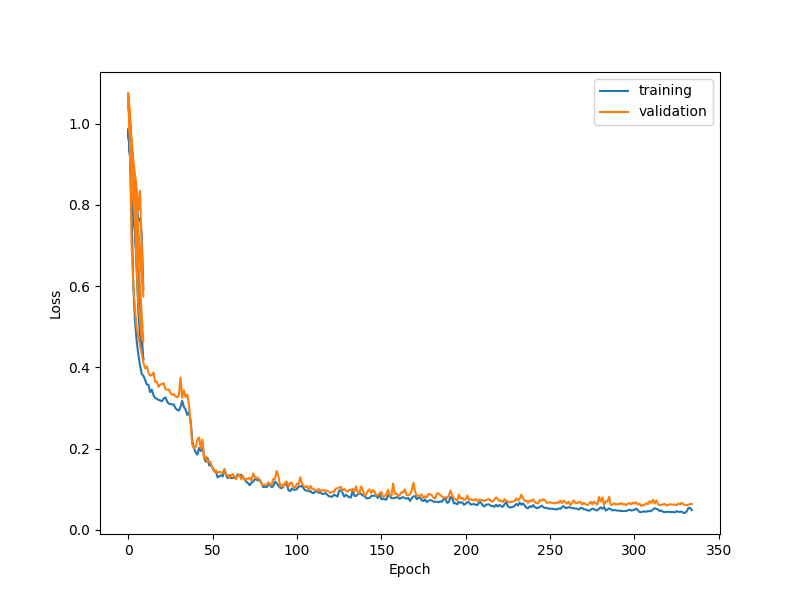
\includegraphics[width=\textwidth]{./project3/figures/figure1a.png}
        \caption{Extensive Training on Target Task} 
        \label{subfig3-1:extensive}
    \end{subfigure}\hfill
    \begin{subfigure}{0.48\textwidth}
        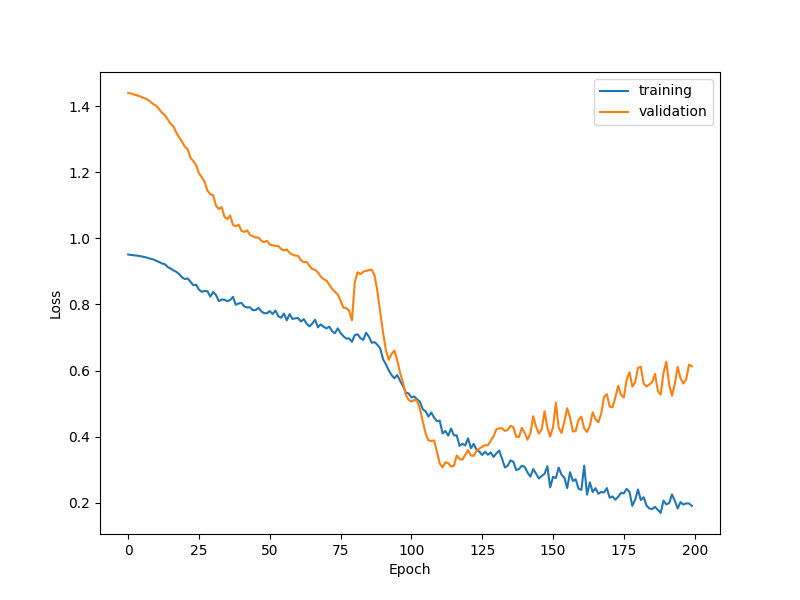
\includegraphics[width=\textwidth]{./project3/figures/figure1b.png}
        \caption{Without TL}
        \label{subfig3-1:without}
    \end{subfigure}
    \begin{subfigure}{0.48\textwidth}
        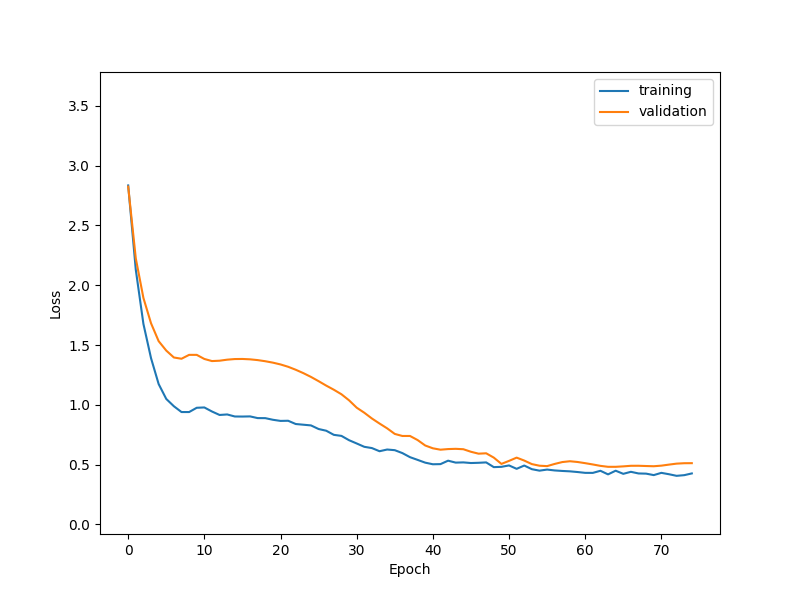
\includegraphics[width=\textwidth]{./project3/figures/figure1c.png}
        \caption{With Fine-tuning}
        \label{subfig3-1:fineTuning}
    \end{subfigure}\hfill
    \begin{subfigure}{0.48\textwidth}
        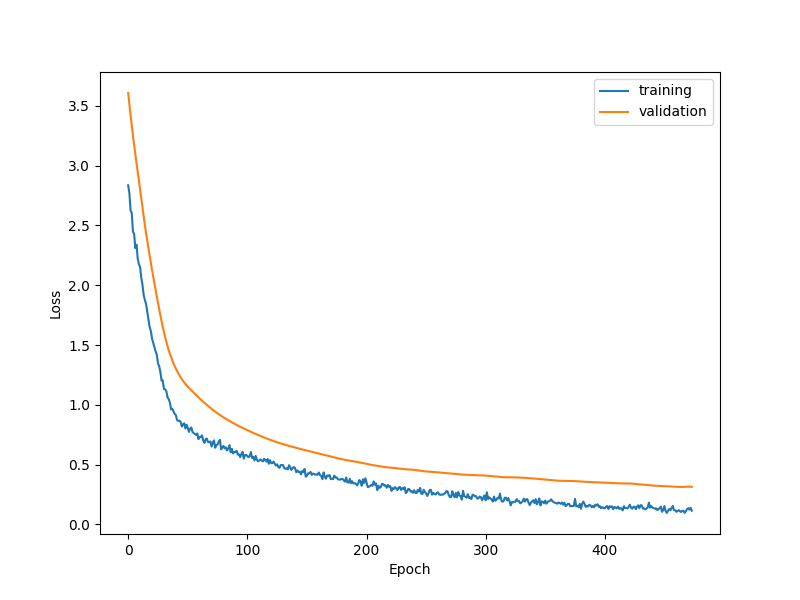
\includegraphics[width=\textwidth]{./project3/figures/figure1d.png}
        \caption{With Layer Freezing}
        \label{subfig3-1:layerFreezing}
    \end{subfigure}
    \caption{Metamodel performance on RS-GBM GMMB with static lapse}
    \label{fig3:figure1}
\end{figure}

We first examine the performance of fine-tuning and layer freezing in adapting LSTM metamodels to new VA contracts with lapse features.
Figure~\ref{fig3:figure1} compares the performance of LSTM metamodels on the target tasks with and without TL.
Learning histories of the LSTM metamodels is shown for the target task of metamodeling GMMB contract losses on the RS-GBM asset model with static lapse.
The source task is hedging a GMMB contract on RS-GBM with no lapse, and the target task is hedging the same GMMB contract but with static lapse.
The simulation data for the target task is generated with the same nested simulation simulation procedure as the source task, except for the lapse feature.
Figure~\ref{subfig3-1:extensive} demonstrates the performance of the LSTM metamodel trained extensively only on the target task using $M_{\text{TA}} = 50,\!000$ samples, which serves as a benchmark for this study. 
The metamodel achieves a low validation MSE due to the availability of a large dataset.
In contrast, Figure~\ref{subfig3-1:without} presents the results of training directly on the target task without pre-training on the source task.
With $M_{\text{TA}} = 2,\!000$ samples, the LSTM metamodel struggles to learn the temporal dependencies and patterns in the target task.
It leads to highly unstable training dynamics, with substantial fluctuations in the validation MSE.
Learning without knowledge transfer leads poor generalization and extreme overfitting. 
Often, the training data is limited for a new VA contract, and such instability is particularly problematic for quick adaptation of LSTM metamodels.
TL techniques like fine-tuning and layer freezing can help mitigate these challenges.
Figure~\ref{subfig3-1:fineTuning} shows the results of fine-tuning a pretrained metamodel on RS-GBM with no lapse.
Fine-tuning offers a noticeable improvement over training without TL by reducing the instability in the validation MSE. 
However, despite this improvement, fine-tuning may not fully mitigate the challenges of training with a small dataset.
The fine-tuned metamodel struggles to achieve a low validation MSE.
Lowering the learning rate does not help the fine-tuned metamodel converge, and the validation MSE remains high after increasing the number of training epochs.
It indicates that fine-tuning may not be sufficient for limited training data.
Figure~\ref{subfig3-1:layerFreezing} presents the performance of layer freezing on the same target task.
Layer freezing offers a more stable training process compared to fine-tuning, with a lower validation error and reduced fluctuations during its training.
The LSTM layers are critical for capturing general feature representations that are transferable across tasks, and freezing these layers helps prevent overfitting to the target task.
In addition, the layer freezing approch tunes fewer neural network parameters than crude fine-tuning.
It allows the transferred metamodelmodel to only focus on learning the lapse features without excessively adjusting the general temporal representations learned from the source task.
This reduction in trainable parameters also accelerates the convergence process, and it leads to a more stable and efficient training on the target task.

\subsection{Transfer to VAs with Dynamic Lapse}

\begin{figure}[ht!]
    \centering
    \begin{subfigure}{0.48\textwidth}
        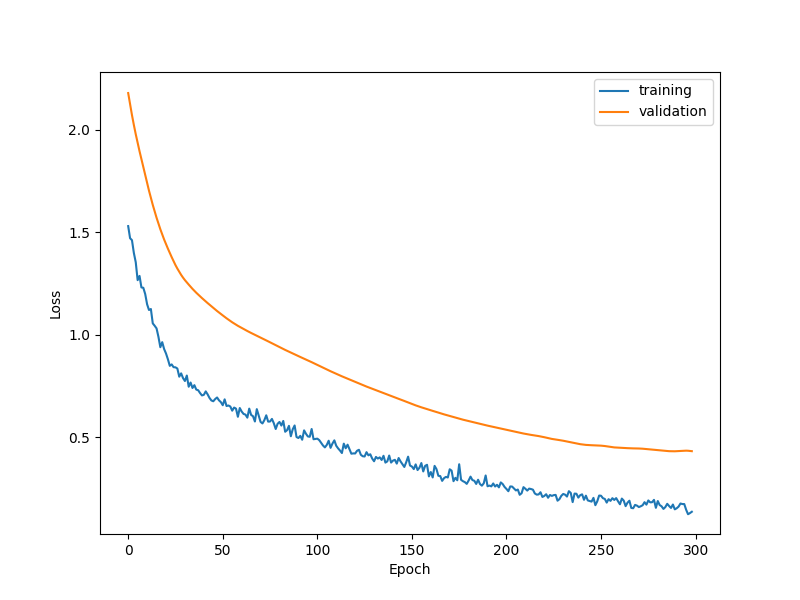
\includegraphics[width=\textwidth]{./project3/figures/figure2a.png}
        \caption{Fine-tuning from No Lapse} 
        \label{subfig3-2:fromNolapse}
    \end{subfigure}\hfill
    \begin{subfigure}{0.48\textwidth}
        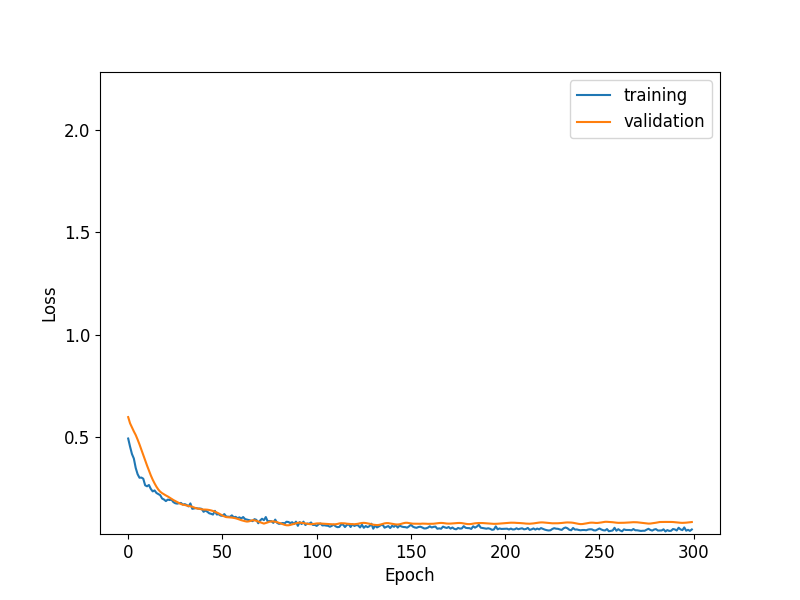
\includegraphics[width=\textwidth]{./project3/figures/figure2b.png}
        \caption{Fine-tuning from Static Lapse}
        \label{subfig3-2:fromLapse}
    \end{subfigure}
    \caption{Fine-tuned Metamodel performance on RS-GBM GMMB with dynamic lapse}
    \label{fig3:figure2}
\end{figure}

We further investigate the performance of fine-tuning on the target task of metamodeling GMMB contract losses on RS-GBM with dynamic lapse. 
The source tasks used for pretraining are GMMB contracts on RS-GBM with no lapse and static lapse, respectively. 
Figure~\ref{fig3:figure2} displays the learning curves of the LSTM metamodels fine-tuned from these two distinct source tasks.
We observe that the performance of the fine-tuned metamodel is highly dependent on the similarity between the source and target tasks.
Fine-tuning from a source task with static lapse results in faster convergence and lower validation error.
The metamodel trained on the GMMB with static lapse captures some features that are beneficial for the GMMB with dynamic lapse, which leads to a more stable training process.
In Figure~\ref{subfig3-2:fromNolapse}, the metamodel needs to learn the effect of (1) whether lapse is present and (2) whether the lapse is dynamic.
This learning process is more challenging.

The observed improvement in transferability when fine-tuning from a static lapse source task highlights the importance of selecting appropriate source tasks in TL. 
When the source task diverges significantly from the target task, the transferred metamodel may struggle to adapt to the new conditions given the limited amount of of training data.

\begin{figure}[ht!]
    \centering
    \begin{subfigure}{0.48\textwidth}
        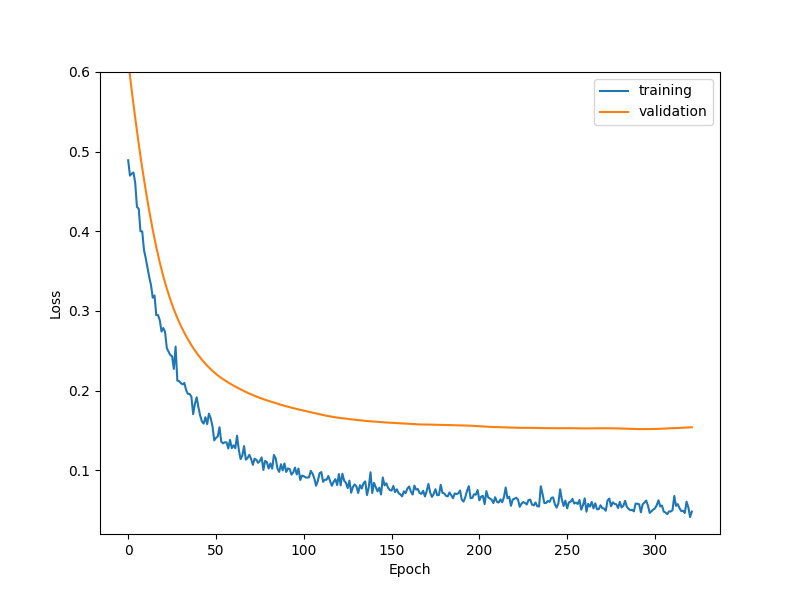
\includegraphics[width=\textwidth]{./project3/figures/figure3a.png}
        \caption{Freezing LSTM Layers} 
        \label{subfig3-3:freezeLSTM}
    \end{subfigure}\hfill
    \begin{subfigure}{0.48\textwidth}
        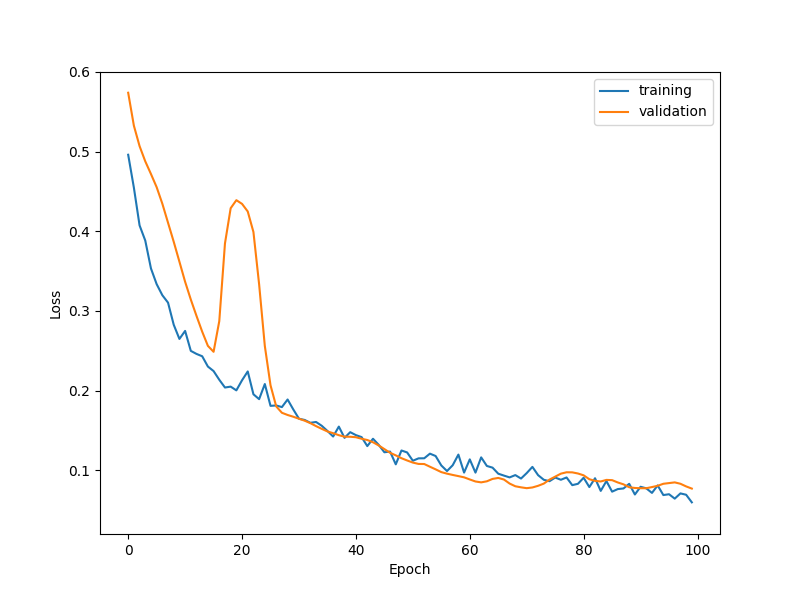
\includegraphics[width=\textwidth]{./project3/figures/figure3b.png}
        \caption{Freezing the Fully Connected Layer}
        \label{subfig3-3:freezeFC}
    \end{subfigure}
    \caption{Layer Freezing on RS-GBM GMMB with dynamic lapse}
    \label{fig3:figure3}
\end{figure}

Figure~\ref{fig3:figure3} continues the investigation of layer freezing in the task of metamodeling GMMB contract losses on RS-GBM with dynamic lapse. 
When transferring knowledge from the GMMB model with static lapse, the primary adaptation for the target task involves learning the impact of dynamic lapse.
Freezing the LSTM layers and fine-tuning only the fully connected layer results in a higher validation error, which suggests a tendency of overfitting.
This indicates that the fully connected layer struggles to adapt to the changes in the temporal dynamics introduced by dynamic lapse, which can be viewed as another source of randomness in the time series.
In contrast, freezing the fully connected layer and fine-tuning the LSTM layers leads to a lower validation error and better generalization. 
This can be attributed to the fact that the LSTM layers are responsible for capturing the temporal dependencies associated with dynamic lapse, and the fully connected layer predicts the contract losses based on these learned features.

This experiment emphasizes the importance of choosing which layers to freeze based on the nature of the source and target tasks. 
In the case of learning dynamic lapse features, freezing the LSTM layers is not beneficial as they need to adapt to the new temporal patterns.

\begin{table}[ht!]
    \centering
    \begin{tabular}{lllll}
    \toprule
    \textbf{Source} & \textbf{Extensive} & \textbf{Fine-tuning} & \textbf{Layer Freezing} & \textbf{Without TL} \\
    \midrule
    No Lapse GMMB & N/A & 0.4894 & 0.3361 & N/A \\
    Static Lapse GMMB & N/A & 0.0794 & 0.0763 & N/A \\
    Dynamic Lapse GMMB & 0.0587 &  N/A &  N/A & 0.2950 \\
    \bottomrule
    \end{tabular}
    \caption{Comparison of different TL methods on GMMB contracts}
    \label{tab3:transfer_learning_results}
\end{table}

Table~\ref{tab3:transfer_learning_results} summarizes the true MSEs of the LSTM metamodels trained using different TL methods across various source tasks.
The calculations are based on the metamodel predictions and the true contract losses approximated with $100,\!000$ inner replications.
The first two rows show the performance of transferring knowledge from GMMB contracts with no lapse and static lapse to the target task of GMMB with dynamic lapse.
The last row shows the performance of training without TL on the target task.
The results demonstrate the effectiveness of fine-tuning and layer freezing in transferring knowledge from a related source tasks to the target task. 
When transferring from a source task with static lapse to a target task with dynamic lapse, the MSEs achieved are $0.0794$ for fine-tuning and $0.0763$ for layer freezing.
The benchmark MSE of $0.0587$, obtained from extensive training on the GMMB dynamic lapse task with much more samples.
While TL from static lapse GMMB do not reach this level of accuracy due to the limited data in the target task, they significantly outperform training without TL. 
This indicates that the models pre-trained on a static lapse setting are effective in capturing relevant features that are transferable to the dynamic lapse scenario.

However, when the source task is less similar to the target task, the benefits of TL are less pronounced. The MSEs in this case are higher, with fine-tuning resulting in $0.4894$ and layer freezing achieving $0.3361$. 
This suggests that the divergence between the source and target tasks can lead to negative transfer.
These results highlight the importance of selecting source tasks that share significant similarities with the target task to maximize the effectiveness of TL. 
When the source and target contracts are substantially different, the pre-trained metamodels may struggle to adapt to the new conditions, as they may not have learned features relevant to the target task.

\subsection{Transfer Knowledge to other Contract Types}

When transferring knowledge from one VA contract type to another, the LSTM metamodel needs to adapt to different contract features and time series dynamics.
We consider the task of metamodeling GMWB contract losses on RS-GBM asset model with dynamic lapse, with the source tasks being a GMMB contract on RS-GBM also with dynamic lapse.
Figure~\ref{fig3:figure4} illustrates the learning history of transferring pre-trained LSTM metamodels from the GMMB contracts to the GMWB contracts.

\begin{figure}[ht!]
    \centering
    \begin{subfigure}{0.48\textwidth}
        \includegraphics[width=\textwidth]{./project3/figures/figure4a.png}
        \caption{Extensive Training on Target Task} 
        \label{subfig3-4:extensive}
    \end{subfigure}\hfill
    \begin{subfigure}{0.48\textwidth}
        \includegraphics[width=\textwidth]{./project3/figures/figure4b.png}
        \caption{Without TL}
        \label{subfig3-4:without}
    \end{subfigure}
    \begin{subfigure}{0.48\textwidth}
        \includegraphics[width=\textwidth]{./project3/figures/figure4c.png}
        \caption{With Fine-tuning}
        \label{subfig3-4:fineTuning}
    \end{subfigure}\hfill
    \begin{subfigure}{0.48\textwidth}
        \includegraphics[width=\textwidth]{./project3/figures/figure4d.png}
        \caption{With Layer Freezing}
        \label{subfig3-4:layerFreezing}
    \end{subfigure}
    \caption{TL performance on RS-GBM GMWB with dynamic lapse}
    \label{fig3:figure4}
\end{figure}

Figure~\ref{subfig3-4:extensive} presents the performance of an extensively trained LSTM metamodel on the target task using 50,000 samples, serving as a benchmark of best metamodel performance. 
The extensively trained metamodel achieves a low validation error and demonstrates stable convergence due to having enough training samples. 
In contrast, Figure~\ref{subfig3-4:without} shows the results of training the metamodel directly on the target task with $2,\!000$ training samples. 
Fewer training samples and no prior knowledge leads to unstable training dynamics. 
The validation MSE fluctuates significantly.

When applying fine-tuning from the GMMB source task (Figure~\ref{subfig3-4:fineTuning}), the metamodel exhibits improved performance compared to training without TL. 
Fine-tuning results in a lower validation error and more stable convergence.
Despite the differences between GMMB and GMWB contracts, there is still valuable information that can be transferred. 
Both the LSTM layers and the fully connected layers capture general temporal patterns and feature representations that are beneficial for the target task. 
Fine-tuning allows the metamodel to adjust all its neural network layers. 
It allows better adaptation to the complexities introduced by the GMWB contract.

However, when employing layer freezing (Figure~\ref{subfig3-4:layerFreezing}), the metamodel's performance deteriorates.
Freezing some layers trained on the GMMB contracts does not allow the metamodel to sufficiently adapt to the complexities of the GMWB contracts. 
The GMWB contracts are inherently more complex than GMMB contracts due to the guaranteed withdrawal benefits at each time step, and the contract features are significantly different.
The complexity introduce significant changes in the time series dynamics that the metamodel needs to capture.
Freezing the LSTM layers or the fully connected layer hinders the metamodel's ability to learn these new patterns, and it leads to poor generalization and unstable error curves.

\begin{table}[ht!]
    \centering
    \begin{tabular}{lrr}
        \toprule
        \textbf{Model} & \textbf{Training MSE} & \textbf{True MSE} \\
        \midrule
        Without TL & 0.3588 & 0.4188 \\
        Fine Tuning & 0.1690 & 0.1780 \\
        Layer Freezing & 0.1828 & 0.2295 \\
        Extensive Training & 0.0853 & 0.0726 \\
        \bottomrule
    \end{tabular}
    \caption{Comparison of different TL methods on GMWB contracts}
    \label{tab3:transfer_learning_results_gmwb}
\end{table}

Table~\ref{tab3:transfer_learning_results_gmwb} summarizes the true MSEs of the LSTM metamodels on the GMWB contracts.
The suboptimal performance of layer freezing in this context indicates that the difference between the source and target tasks is too substantial for this method to be effective. 
While layer freezing can be advantageous when the source and target tasks are closely related, it may hinder performance when the tasks diverge significantly.
In such circumstances, fine-tuning provides a better approach by allowing the metamodel to leverage transferable knowledge while adapting to the new task's specific requirements. 
Fine-tuning enables both the LSTM and fully connected layers to update their weights, capturing the complex dynamics of the GMWB contracts more effectively.
This is particularly beneficial when developing metamodels for complex VA contracts with limited simulation data. 
For instance, transferring information from GMMB contracts can still be valuable when modeling GMWB contracts.
Both contracts share some common contract features and temporal patterns, which allows a pre-trained LSTM metamodel to capture generalizable features that provide a solid foundation for the target task.

\begin{figure}[ht!]
    \centering
    \begin{subfigure}{0.48\textwidth}
        \includegraphics[width=\textwidth]{./project3/figures/figure4_1.png}
        \caption{Tail scenarios identification} 
        \label{subfig3-4-1:tail}
    \end{subfigure}\hfill
    \begin{subfigure}{0.48\textwidth}
        \includegraphics[width=\textwidth]{./project3/figures/figure4_2.png}
        \caption{$95\%$-CVaR prediction}
        \label{subfig3-4-2:CVaR}
    \end{subfigure}
    \caption{TL performance on RS-GBM GMWB with dynamic lapse}
    \label{fig3:figure4-1}
\end{figure}

Figure~\ref{fig3:figure4-1} illustrates the performance of the two-stage procedure with TL for GMWB contracts with dynamic lapse in predicting the tail scenarios and the $95\%$-CVaR.
The graph provides a visual representation of how different TL approaches compare to training from scratch and the standard nested simulation procedure.
Fine-tuning consistently outperforms both layer freezing and training from scratch across different simulation budgets, particularly in predicting tail scenarios and estimating the 95\%-CVaR. 
This finding is consistent with the training history and MSEs in Figure~\ref{fig3:figure4} and Table~\ref{tab3:transfer_learning_results_gmwb}, respectively.
It's important to note that while these results are promising, they also highlight the complexity of modeling GMWB contracts with dynamic lapse. 
The fact that fine-tuning outperforms layer freezing suggests that there are significant differences in the tail behavior of GMMB and GMWB contracts, particularly when dynamic lapse is considered. 
This underscores the need for careful model selection and validation when applying TL techniques to different VA products.

\subsection{Multi-task Learning}

Multi-task learning enables the LSTM metamodels to learn shared representations across related VA contracts.
In this section, we examine the performance of multitask learning applied to two types of VAs, GMMB and GMWB with dynamic lapse rates.
The simulation datasets contrain $2,\!000$ samples for each contract type, and the LSTM metamodels are trained using multi-task learning. 
In our experiments, Algorithm~\ref{alg3:multiTaskLearning} is used to train the LSTM metamodels simultaneously to minimize the multi-task MSE loss function in Equation~\ref{eq3:multiTaskLoss}.
We use individual task training as a baseline for comparison, where the LSTM metamodels are trained separately on the GMMB and GMWB contracts.
The objective is to assess how multitask learning can improve the training efficiency and performance of both products compared to individual task training.

\begin{figure}[ht!]
    \includegraphics[width=\textwidth]{./project3/tikz/mtl.pdf}
    \caption{Multi-task Learning Framework for VA Contracts}
    \label{fig3:mtl}
\end{figure}

Figure~\ref{fig3:mtl} illustrates our multi-task learning framework for GMMB and GMWB contracts with dynamic lapse rates.
The outer simulation paths for both contracts are the same, which are generated from the same nested simulation procedure with $100$ inner replications.
The LSTM metamodels are trained simultaneously on both contracts.
The LSTM layers are shared, and each contract has its own separate fully connected layers for contract loss predictions.

\begin{figure}[ht!]
    \centering
    \begin{subfigure}{0.48\textwidth}
        \includegraphics[width=\textwidth]{./project3/figures/figure5a.png}
        \caption{Multi-task training history} 
        \label{subfig3-5:multiTask}
    \end{subfigure}\hfill
    \begin{subfigure}{0.48\textwidth}
        \includegraphics[width=\textwidth]{./project3/figures/figure5b.png}
        \caption{Task performance with multitask training}
        \label{subfig3-5:fineTuning}
    \end{subfigure}
    \begin{subfigure}{0.48\textwidth}
        \includegraphics[width=\textwidth]{./project3/figures/figure5c.png}
        \caption{GMMB individual task training} 
    \label{subfig3-5:gmmb_individual}
    \end{subfigure}\hfill
    \begin{subfigure}{0.48\textwidth}
        \includegraphics[width=\textwidth]{./project3/figures/figure5d.png}
        \caption{GMWB individual task training}
        \label{subfig3-5:gmwb_individual}
    \end{subfigure}
    \caption{Multi-task Learning on RS-GBM GMMB and GMWB with dynamic lapse}
    \label{fig3:figure5}
\end{figure}

Figure~\ref{fig3:figure5} compares the learning curves for the training of GMMB and GMWB, with and without multitask learning.
The comparison between multitask learning (Figure~\ref{subfig3-5:multiTask} and~\ref{subfig3-5:fineTuning}) and individual task training ((Figure~\ref{subfig3-5:gmmb_individual} and~\ref{subfig3-5:gmwb_individual})) demonstrates the benefit of multi-task learning for both products. 
In the case of GMMB, multitask learning allows the model to achieve faster convergence while reducing overfitting.
For GMWB, the multi-task learning framework helps to stablize the training process.
The shared LSTM layers in the multitask model are able to capture common temporal patterns and dynamics, which benefits both GMMB and GMWB when training samples is scarce.
Similar to pooling in Chapter~\ref{chap:project1} and~\ref{chap:project2} but on a higher level, multi-task learning enables the LSTM metamodels to leverage shared representations across related VA contracts.

% \begin{figure}[ht!]
%     \centering
%     \begin{subfigure}{0.48\textwidth}
%         \includegraphics[width=\textwidth]{./project3/figures/figure5a.png}
%         \caption{Multi-task training history} 
%         \label{subfig3-6:multiTask}
%     \end{subfigure}\hfill
%     \begin{subfigure}{0.48\textwidth}
%         \includegraphics[width=\textwidth]{./project3/figures/figure5b.png}
%         \caption{Task performance with multitask training}
%         \label{subfig3-6:fineTuning}
%     \end{subfigure}    
%     \label{fig3:figure6}
% \end{figure}

% Even when data is abundant, multi-task learning can improve the training efficiency and predictive performance of LSTM metamodels for nested simulations.
% The shared LSTM layers learn generalizable features that are beneficial across different VA contracts.
% Figure~\ref{fig3:figure6} demonstrates the performance of multi-task learning on GMMB and GMWB contracts with dynamic lapse rates.

\section{Conclusion} \label{sec3:conclusion}

In this chapter, we introduced a transfer learning framework to accelerate the training of LSTM metamodels for dynamic hedging of variable annuity contracts.
Traditional nested simulation procedures for VA risk management are computationally intensive.
LSTM metamodels offer a data-driven approach to approximate the true contract losses, which can significantly reduce the computational cost of hedging a single VA contract.
However, training LSTM metamodels on new VA contracts can be challenging due to the limited availability of simulation data.
Our proposed framework leverages pre-trained LSTM networks and transfer learning techniques to adapt quickly metamodels to new but related VA contracts with minimal additional simulation cost.
Fine-tuning a pre-trained LSTM metamodel on a new target task with limited data significantly improved training stability and predictive accuracy compared to training from scratch. 
Layer freezing further enhanced performance by retaining transferable temporal representations learned from the source task. 
However, the success of these methods depends on the similarity between the source and target tasks. 
When the tasks were closely related, freezing some neural network layers yields substantial benefits. 
Conversely, when the source and target tasks diverged significantly, fine-tuning the entire network is more effective.

Multi-task learning offers a robust framework for transferring knowledge across related simulation schemes in LSTM metamodeling for nested simulations. 
By sharing representations through the LSTM layers, the model can learn more generalizable features that are beneficial across different VA contracts. 
The multi-task approach was particularly beneficial when training data for individual tasks was scarce, as it effectively pooled information across tasks to enhance learning efficiency and predictive performance.
Furthermore, a metamodel trained with multi-task learning can serve as a pre-trained model. 
It is adaptable to various VA contracts and asset models, and it is a versatile tool for practical applications in dynamic hedging of VAs.

The integration of transfer learning into LSTM metamodeling represents a significant advancement in robust risk management associated with variable annuity contracts.
By effectively leveraging existing knowledge, financial institutions can maintain accurate and responsive risk management practices in a rapidly changing market environment. 
The methodologies presented in this chapter attempt to make a significant contribution to the broader applications of transfer learning in financial modeling and risk assessment.



%----------------------------------------------------------------------
% END MATERIAL
%----------------------------------------------------------------------

% B I B L I O G R A P H Y
% -----------------------

% The following statement selects the style to use for references.  It controls the sort order of the entries in the bibliography and also the formatting for the in-text labels.
\bibliographystyle{apalike}
% This specifies the location of the file containing the bibliographic information.  
% It assumes you're using BibTeX (if not, why not?).
\cleardoublepage % This is needed if the book class is used, to place the anchor in the correct page,
                 % because the bibliography will start on its own page.
                 % Use \clearpage instead if the document class uses the "oneside" argument
\phantomsection  % With hyperref package, enables hyperlinking from the table of contents to bibliography             
% The following statement causes the title "References" to be used for the bibliography section:
\renewcommand*{\bibname}{References}

% Add the References to the Table of Contents
\addcontentsline{toc}{chapter}{\textbf{References}}

\bibliography{refP1, refP2, refP3}
% Tip 5: You can create multiple .bib files to organize your references. 
% Just list them all in the \bibliogaphy command, separated by commas (no spaces).

% The following statement causes the specified references to be added to the bibliography% even if they were not 
% cited in the text. The asterisk is a wildcard that causes all entries in the bibliographic database to be included (optional).
\nocite{*}

\chapter*{Appendix} \label{chap:appendix}

\section{Connections between Convergence in MSE and AE}\label{appendix:connection-mse-absolute-error}

This section establishes the connections between the convergence in \gls{mse} and the convergence in probabilistic order for \gls{ae} in the context of nested simulation procedures.
In order to show the connections between the convergence in \gls{mse} and the convergence in probabilistic order for \gls{ae}, we first need to state the definition for a sequence of random variables to converge in those two forms.

\begin{definition}
    Let $\hat{\rho}_{\Gamma}$ be an estimator of $\rho$ with a simulation budget of $\Gamma$. 
    We write $\mathbb{E} \left[ \left(\hat{\rho}_{\Gamma} - \rho\right)^2 \right] = \mathcal{O} \left( \Gamma^{-\xi} \right)$, that is, $\hat{\rho}_{\Gamma}$ converges in \gls{mse} to $\rho$ in order $\xi$ if there exists a constant $C$ such that
    $$
        \limsup_{\Gamma \to \infty} \frac{\mathbb{E} \left[\left(\hat{\rho}_{\Gamma} - \rho\right)^2 \right]}{\Gamma^{-\xi}} \leq C.
    $$
\end{definition}

\begin{definition}
    Let $\hat{\rho}_{\Gamma}$ be an estimator of $\rho$ with a simulation budget of $\Gamma$. 
    We write $|\hat{\rho}_{\Gamma} - \rho| = \mathcal{O}_{\mathbb{P}}(\Gamma^{-\xi})$, that is $\hat{\rho}_{\Gamma}$ converges in probabilistic order $\xi$ to $\rho$ if for a sufficiently large $\Gamma$, for any $\epsilon > 0$ there exists a $C$ such that
    $$
         \mathbb{P} \left( \left| \hat{\rho}_{\Gamma} - \rho \right| \geq C \Gamma^{-\xi} \right) \leq \epsilon.
    $$
\end{definition}

We start our analysis by showing the convergence in probabilistic order from the convergence in \gls{mse}.
Let $\hat{\rho}_{\Gamma}$ be an estimator of $\rho$ with a simulation budget of $\Gamma$, and assume that $\mathbb{E} \left[ \left(\hat{\rho}_{\Gamma} - \rho\right)^2 \right] = \mathcal{O} \left( \Gamma^{-\xi-\delta} \right)$ for an arbitrarily small $\delta > 0$.
Then, from the definition of convergence in \gls{mse}, 
$$
    \limsup_{\Gamma \to \infty} \frac{\mathbb{E} \left[ \left(\hat{\rho}_{\Gamma} - \rho\right)^2 \right]}{\Gamma^{-\xi-\delta}} \leq C.
$$
for a constant $C > 0$.

The above inequality implies that
$$
\limsup_{\Gamma \to \infty} \frac{\mathbb{E} \left[ \left(\hat{\rho}_{\Gamma} - \rho\right)^2 \right]}{\Gamma^{-\xi}} =0.
$$

Therefore, by Chebyshev's inequality, for any $\epsilon > 0$, we have
$$
\mathbb{P} \left( \left| \hat{\rho}_{\Gamma} - \rho \right| \Gamma^{\xi/2} > C  \right) \leq \frac{\mathbb{E} \left[ \left(\hat{\rho}_{\Gamma} - \rho\right)^2 \Gamma^{\xi} \right]}{C^2 } \rightarrow 0 
$$
as $\Gamma \to \infty$.

Therefore, $\hat{\rho}_{\Gamma}$ converges in probabilistic order $\xi/2$ to $\rho$ as $\Gamma \to \infty$, that is,
$$
\left| \hat{\rho}_{\Gamma} - \rho \right| = \mathcal{O}_{\mathbb{P}} \left( \Gamma^{-\xi/2} \right).
$$


\end{document}
